
%% bare_jrnl.tex
%% V1.4
%% 2012/12/27
%% by Michael Shell
%% see http://www.michaelshell.org/
%% for current contact information.
%%
%% This is a skeleton file demonstrating the use of IEEEtran.cls
%% (requires IEEEtran.cls version 1.8 or later) with an IEEE journal paper.
%%
%% Support sites:
%% http://www.michaelshell.org/tex/ieeetran/
%% http://www.ctan.org/tex-archive/macros/latex/contrib/IEEEtran/
%% and
%% http://www.ieee.org/



% *** Authors should verify (and, if needed, correct) their LaTeX system  ***
% *** with the test flow diagnostic prior to trusting their LaTeX platform ***
% *** with production work. IEEE's font choices can trigger bugs that do  ***
% *** not appear when using other class files.                            ***
% The test flow support page is at:
% http://www.michaelshell.org/tex/testflow/


%%*************************************************************************
%% Legal Notice:
%% This code is offered as-is without any warranty either expressed or
%% implied; without even the implied warranty of MERCHANTABILITY or
%% FITNESS FOR A PARTICULAR PURPOSE! 
%% User assumes all risk.
%% In no event shall IEEE or any contributor to this code be liable for
%% any damages or losses, including, but not limited to, incidental,
%% consequential, or any other damages, resulting from the use or misuse
%% of any information contained here.
%%
%% All comments are the opinions of their respective authors and are not
%% necessarily endorsed by the IEEE.
%%
%% This work is distributed under the LaTeX Project Public License (LPPL)
%% ( http://www.latex-project.org/ ) version 1.3, and may be freely used,
%% distributed and modified. A copy of the LPPL, version 1.3, is included
%% in the base LaTeX documentation of all distributions of LaTeX released
%% 2003/12/01 or later.
%% Retain all contribution notices and credits.
%% ** Modified files should be clearly indicated as such, including  **
%% ** renaming them and changing author support contact information. **
%%
%% File list of work: IEEEtran.cls, IEEEtran_HOWTO.pdf, bare_adv.tex,
%%                    bare_conf.tex, bare_jrnl.tex, bare_jrnl_compsoc.tex,
%%                    bare_jrnl_transmag.tex
%%*************************************************************************

% Note that the a4paper option is mainly intended so that authors in
% countries using A4 can easily print to A4 and see how their papers will
% look in print - the typesetting of the document will not typically be
% affected with changes in paper size (but the bottom and side margins will).
% Use the test flow package mentioned above to verify correct handling of
% both paper sizes by the user's LaTeX system.
%
% Also note that the "draftcls" or "draftclsnofoot", not "draft", option
% should be used if it is desired that the figures are to be displayed in
% draft mode.
%
\documentclass[journal,onecolumn]{IEEEtran}
%
% If IEEEtran.cls has not been installed into the LaTeX system files,
% manually specify the path to it like:
% \documentclass[journal]{../sty/IEEEtran}





% Some very useful LaTeX packages include:
% (uncomment the ones you want to load)


% *** MISC UTILITY PACKAGES ***
%
%\usepackage{ifpdf}
% Heiko Oberdiek's ifpdf.sty is very useful if you need conditional
% compilation based on whether the output is pdf or dvi.
% usage:
% \ifpdf
%   % pdf code
% \else
%   % dvi code
% \fi
% The latest version of ifpdf.sty can be obtained from:
% http://www.ctan.org/tex-archive/macros/latex/contrib/oberdiek/
% Also, note that IEEEtran.cls V1.7 and later provides a builtin
% \ifCLASSINFOpdf conditional that works the same way.
% When switching from latex to pdflatex and vice-versa, the compiler may
% have to be run twice to clear warning/error messages.
\usepackage{enumitem}
% enumitem enables enumerations with letters
\usepackage{threeparttable}
% threeparttable for tables with both captions and notes
\usepackage{afterpage}



% *** CITATION PACKAGES ***
%
%\usepackage{cite}
% cite.sty was written by Donald Arseneau
% V1.6 and later of IEEEtran pre-defines the format of the cite.sty package
% \cite{} output to follow that of IEEE. Loading the cite package will
% result in citation numbers being automatically sorted and properly
% "compressed/ranged". e.g., [1], [9], [2], [7], [5], [6] without using
% cite.sty will become [1], [2], [5]--[7], [9] using cite.sty. cite.sty's
% \cite will automatically add leading space, if needed. Use cite.sty's
% no adjust option (cite.sty V3.8 and later) if you want to turn this off
% such as if a citation ever needs to be enclosed in parenthesis.
% cite.sty is already installed on most LaTeX systems. Be sure and use
% version 4.0 (2003-05-27) and later if using hyperref.sty. cite.sty does
% not currently provide for hyperlinked citations.
% The latest version can be obtained at:
% http://www.ctan.org/tex-archive/macros/latex/contrib/cite/
% The documentation is contained in the cite.sty file itself.






% *** GRAPHICS RELATED PACKAGES ***
%
\usepackage{graphicx}
% declare the path(s) where your graphic files are
\graphicspath{{images/}}
% and their extensions so you won't have to specify these with
% every instance of \includegraphics
\DeclareGraphicsExtensions{.pdf,.jpeg,.png}
% graphics was written by David Carlisle and Sebastian Rahtz. It is
% required if you want graphics, photos, etc. graphicx.sty is already
% installed on most LaTeX systems. The latest version and documentation
% can be obtained at: 
% http://www.ctan.org/tex-archive/macros/latex/required/graphics/
% Another good source of documentation is "Using Imported Graphics in
% LaTeX2e" by Keith Reckdahl which can be found at:
% http://www.ctan.org/tex-archive/info/epslatex/
%
% latex, and pdflatex in dvi mode, support graphics in encapsulated
% postscript (.eps) format. pdflatex in pdf mode supports graphics
% in .pdf, .jpeg, .png and .mps (metapost) formats. Users should ensure
% that all non-photo figures use a vector format (.eps, .pdf, .mps) and
% not a bitmapped formats (.jpeg, .png). IEEE frowns on bitmapped formats
% which can result in "jaggedy"/blurry rendering of lines and letters as
% well as large increases in file sizes.
%
% You can find documentation about the pdfTeX application at:
% http://www.tug.org/applications/pdftex

\usepackage[export]{adjustbox}
% adjustbox used as a convenience tool for drawing frames around images

\usepackage{pgfplots}
% pgfplots for graphing functions

\usepackage{tikz}
\usetikzlibrary{fit}
\usetikzlibrary{calc}
\usetikzlibrary{arrows}
\usetikzlibrary{positioning}
% TikZ enabled us to draw graphics directly in LaTeX

\usepackage{color}
\definecolor{alizarin}{RGB}{231, 76, 60}
\definecolor{pomegranate}{RGB}{192, 57, 43}
\definecolor{emerald}{RGB}{46, 204, 113}
\definecolor{turquoise}{RGB}{26, 188, 156}
\definecolor{greensea}{RGB}{22, 160, 133}
\definecolor{peter}{RGB}{52, 152, 219}





% *** MATH PACKAGES ***
%
\usepackage[cmex10]{amsmath}
% A popular package from the American Mathematical Society that provides
% many useful and powerful commands for dealing with mathematics. If using
% it, be sure to load this package with the cmex10 option to ensure that
% only type 1 fonts will utilized at all point sizes. Without this option,
% it is possible that some math symbols, particularly those within
% footnotes, will be rendered in bitmap form which will result in a
% document that can not be IEEE Xplore compliant!
%
% Also, note that the ams math package sets \interdisplaylinepenalty to 10000
% thus preventing page breaks from occurring within multiline equations. Use:
%\interdisplaylinepenalty=2500
% after loading ams math to restore such page breaks as IEEEtran.cls normally
% does. amsmath.sty is already installed on most LaTeX systems. The latest
% version and documentation can be obtained at:
% http://www.ctan.org/tex-archive/macros/latex/required/amslatex/math/





% *** SPECIALIZED LIST PACKAGES ***
%
%\usepackage{algorithmic}
% algorithmic.sty was written by Peter Williams and Rogerio Brito.
% This package provides an algorithmic environment of describing algorithms.
% You can use the algorithmic environment in-text or within a figure
% environment to provide for a floating algorithm. Do NOT use the algorithm
% floating environment provided by algorithm.sty (by the same authors) or
% algorithm2e.sty (by Christophe Fiorio) as IEEE does not use dedicated
% algorithm float types and packages that provide these will not provide
% correct IEEE style captions. The latest version and documentation of
% algorithmic.sty can be obtained at:
% http://www.ctan.org/tex-archive/macros/latex/contrib/algorithms/
% There is also a support site at:
% http://algorithms.berlios.de/index.html
% Also of interest may be the (relatively newer and more customizable)
% algorithmicx.sty package by Szasz Janos:
% http://www.ctan.org/tex-archive/macros/latex/contrib/algorithmicx/




% *** ALIGNMENT PACKAGES ***
%
%\usepackage{array}
% Frank Mittelbach's and David Carlisle's array.sty patches and improves
% the standard LaTeX2e array and tabular environments to provide better
% appearance and additional user controls. As the default LaTeX2e table
% generation code is lacking to the point of almost being broken with
% respect to the quality of the end results, all users are strongly
% advised to use an enhanced (at the very least that provided by array.sty)
% set of table tools. array.sty is already installed on most systems. The
% latest version and documentation can be obtained at:
% http://www.ctan.org/tex-archive/macros/latex/required/tools/
\usepackage{float}


% IEEEtran contains the IEEEeqnarray family of commands that can be used to
% generate multiline equations as well as matrices, tables, etc., of high
% quality.




% *** SUBFIGURE PACKAGES ***
%\ifCLASSOPTIONcompsoc
%  \usepackage[caption=false,font=normalsize,labelfont=sf,textfont=sf]{subfig}
%\else
%  \usepackage[caption=false,font=footnotesize]{subfig}
%\fi
% subfig.sty, written by Steven Douglas Cochran, is the modern replacement
% for subfigure.sty, the latter of which is no longer maintained and is
% incompatible with some LaTeX packages including fixltx2e. However,
% subfig.sty requires and automatically loads Axel Sommerfeldt's caption.sty
% which will override IEEEtran.cls' handling of captions and this will result
% in non-IEEE style figure/table captions. To prevent this problem, be sure
% and invoke subfig.sty's "caption=false" package option (available since
% subfig.sty version 1.3, 2005/06/28) as this is will preserve IEEEtran.cls
% handling of captions.
% Note that the Computer Society format requires a larger sans serif font
% than the serif footnote size font used in traditional IEEE formatting
% and thus the need to invoke different subfig.sty package options depending
% on whether compsoc mode has been enabled.
%
% The latest version and documentation of subfig.sty can be obtained at:
% http://www.ctan.org/tex-archive/macros/latex/contrib/subfig/
\usepackage{subcaption}
% Use subcaption instead of subfig (deprecated)



% *** FLOAT PACKAGES ***
%
%\usepackage{fixltx2e}
% fixltx2e, the successor to the earlier fix2col.sty, was written by
% Frank Mittelbach and David Carlisle. This package corrects a few problems
% in the LaTeX2e kernel, the most notable of which is that in current
% LaTeX2e releases, the ordering of single and double column floats is not
% guaranteed to be preserved. Thus, an unlatched LaTeX2e can allow a
% single column figure to be placed prior to an earlier double column
% figure. The latest version and documentation can be found at:
% http://www.ctan.org/tex-archive/macros/latex/base/


%\usepackage{stfloats}
% stfloats.sty was written by Sigitas Tolusis. This package gives LaTeX2e
% the ability to do double column floats at the bottom of the page as well
% as the top. (e.g., "\begin{figure*}[!b]" is not normally possible in
% LaTeX2e). It also provides a command:
%\fnbelowfloat
% to enable the placement of footnotes below bottom floats (the standard
% LaTeX2e kernel puts them above bottom floats). This is an invasive package
% which rewrites many portions of the LaTeX2e float routines. It may not work
% with other packages that modify the LaTeX2e float routines. The latest
% version and documentation can be obtained at:
% http://www.ctan.org/tex-archive/macros/latex/contrib/sttools/
% Do not use the stfloats baseline float ability as IEEE does not allow
% \baselineskip to stretch. Authors submitting work to the IEEE should note
% that IEEE rarely uses double column equations and that authors should try
% to avoid such use. Do not be tempted to use the cuted.sty or midfloat.sty
% packages (also by Sigitas Tolusis) as IEEE does not format its papers in
% such ways.
% Do not attempt to use stfloats with fixltx2e as they are incompatible.
% Instead, use Morten Hogholm'a dblfloatfix which combines the features
% of both fixltx2e and stfloats:
%
% \usepackage{dblfloatfix}
% The latest version can be found at:
% http://www.ctan.org/tex-archive/macros/latex/contrib/dblfloatfix/




%\ifCLASSOPTIONcaptionsoff
%  \usepackage[nomarkers]{endfloat}
% \let\MYoriglatexcaption\caption
% \renewcommand{\caption}[2][\relax]{\MYoriglatexcaption[#2]{#2}}
%\fi
% endfloat.sty was written by James Darrell McCauley, Jeff Goldberg and 
% Axel Sommerfeldt. This package may be useful when used in conjunction with 
% IEEEtran.cls'  captions off option. Some IEEE journals/societies require that
% submissions have lists of figures/tables at the end of the paper and that
% figures/tables without any captions are placed on a page by themselves at
% the end of the document. If needed, the draftcls IEEEtran class option or
% \CLASSINPUTbaselinestretch interface can be used to increase the line
% spacing as well. Be sure and use the no markers option of end float to
% prevent end float from "marking" where the figures would have been placed
% in the text. The two hack lines of code above are a slight modification of
% that suggested by in the end float docs (section 8.4.1) to ensure that
% the full captions always appear in the list of figures/tables - even if
% the user used the short optional argument of \caption[]{}.
% IEEE papers do not typically make use of \caption[]'s optional argument,
% so this should not be an issue. A similar trick can be used to disable
% captions of packages such as subfig.sty that lack options to turn off
% the sub captions:
% For subfig.sty:
% \let\MYorigsubfloat\subfloat
% \renewcommand{\subfloat}[2][\relax]{\MYorigsubfloat[]{#2}}
% However, the above trick will not work if both optional arguments of
% the \subfloat command are used. Furthermore, there needs to be a
% description of each subfigure *somewhere* and end float does not add
% subfigure captions to its list of figures. Thus, the best approach is to
% avoid the use of subfigure captions (many IEEE journals avoid them anyway)
% and instead reference/explain all the subfigures within the main caption.
% The latest version of endfloat.sty and its documentation can obtained at:
% http://www.ctan.org/tex-archive/macros/latex/contrib/endfloat/
%
% The IEEEtran \ifCLASSOPTIONcaptionsoff conditional can also be used
% later in the document, say, to conditionally put the References on a 
% page by themselves.




% *** PDF, URL AND HYPERLINK PACKAGES ***
%
%\usepackage{url}
% url.sty was written by Donald Arseneau. It provides better support for
% handling and breaking URLs. url.sty is already installed on most LaTeX
% systems. The latest version and documentation can be obtained at:
% http://www.ctan.org/tex-archive/macros/latex/contrib/url/
% Basically, \url{my_url_here}.




% *** Do not adjust lengths that control margins, column widths, etc. ***
% *** Do not use packages that alter fonts (such as psalter).         ***
% There should be no need to do such things with IEEEtran.cls V1.6 and later.
% (Unless specifically asked to do so by the journal or conference you plan
% to submit to, of course. )


% correct bad hyphenation here
\hyphenation{op-tical net-works semi-conduc-tor}


\begin{document}

\title{Introduction of a Biologically Plausible \\ Color Descriptor to a Neurodynamical Model \\ of the Primary Visual Cortex}
%
%
% author names and IEEE memberships
% note positions of commas and nonbreaking spaces ( ~ ) LaTeX will not break
% a structure at a ~ so this keeps an author's name from being broken across
% two lines.
% use \thanks{} to gain access to the first footnote area
% a separate \thanks must be used for each paragraph as LaTeX2e's \thanks
% was not built to handle multiple paragraphs
%

\author{Sean Thomas Connolly% <-this % stops a space
\thanks{Author: Sean Thomas Connolly, connolly.st@gmail.com}% <-this % stops a space
\thanks{Advisor: Xavier Otazu,  Computer Vision Center, Computer Science Department, Universitat Autònoma de Barcelona, Barcelona, Spain }% <-this % stops a space% stops a space
\thanks{Submitted: September 2014}}

% note the % following the last \IEEEmembership and also \thanks - 
% these prevent an unwanted space from occurring between the last author name
% and the end of the author line. i.e., if you had this:
% 
% \author{....lastname \thanks{...} \thanks{...} }
%                     ^------------^------------^----Do not want these spaces!
%
% a space would be appended to the last name and could cause every name on that
% line to be shifted left slightly. This is one of those "LaTeX things". For
% instance, "\textbf{A} \textbf{B}" will typeset as "A B" not "AB". To get
% "AB" then you have to do: "\textbf{A}\textbf{B}"
% \thanks is no different in this regard, so shield the last } of each \thanks
% that ends a line with a % and do not let a space in before the next \thanks.
% Spaces after \IEEEmembership other than the last one are OK (and needed) as
% you are supposed to have spaces between the names. For what it is worth,
% this is a minor point as most people would not even notice if the said evil
% space somehow managed to creep in.



% The paper headers
\markboth{Master Thesis Dissertation, Master in Computer Vision, July 2014}%
{Shell \MakeLowercase{\textit{et al.}}: Bare Demo of IEEEtran.cls for Journals}
% The only time the second header will appear is for the odd numbered pages
% after the title page when using the two side option.



% make the title area
\maketitle


\begin{abstract}
We present a computational model of color description \& processing in the primary visual cortex (V1), inspired by current neurobiological understanding. This understanding posits single and double-opponent neurons as fundamental to low level color processing. We offer a novel representation of color by defining these cells' responses and the connections between them, within the framework of a dynamical model of neuronal activity. Our model reproduces perceptual experiences in a number of cases, offering credence to said biological theories.
\end{abstract}

% Note that keywords are not normally used for peer review papers.
\begin{IEEEkeywords}
primary visual cortex, striate cortex, V1, receptive field, single-opponent, double-opponent, color assimilation, color induction
\end{IEEEkeywords}


% For peer review papers, you can put extra information on the cover
% page as needed:
% \ifCLASSOPTIONpeerreview
% \begin{center} \bfseries EDICS Category: 3-BBND \end{center}
% \fi
%
% For peer review papers, this IEEEtran command inserts a page break and
% creates the second title. It will be ignored for other modes.
\IEEEpeerreviewmaketitle



\section{Introduction}

% TODO perhaps the distinction between physical color and perception color is valuable here?

\IEEEPARstart{C}{olor} induction and contrast are two related, opposing, perceptual phenomena. The former is a change in perceived color "toward" a nearby color, while the latter is a change of one color "away" from the nearby color. Neurophysiological research suggests that these phenomena may arise as early in primate vision as the primary visual cortex (V1). It is proposed that the boundaries between two colored regions drive these effects. Specifically, research in the field describes neurons which fire selectively to boundaries between certain colors, so called double-opponent cells, and identifies them as being critically related to the color perceived.

Within, we propose a computational model designed around the current understanding of this biology. We present two implementations, one more biologically accurate, and another more computationally elegant. We explore the behavior of these models with respect to what they can teach us about the assumed biological theories, as well as their application to the field of computer vision.


%%%%%%%%%%%%%%%%%%%%%%%%%%%%%%%%%%%%%%%%%%%%%%%%%%%%%%%%%%%%%%%%
%
% STATE OF THE ART
%
% A bibliographic review on of the problem topic.
%
%%%%%%%%%%%%%%%%%%%%%%%%%%%%%%%%%%%%%%%%%%%%%%%%%%%%%%%%%%%%%%%%
\section{State of the art}


\subsection{Neurobiology}

Historically, it was widely believed that color and shape are two distinct aspects of visual perception. Truly, this line of thinking is intuitive: one can perceive the color of a flat surface which occupies our full field of vision, despite its lack of 'shape', likewise we can see the shape of achromatic objects, as in black and white film. This theory of perception innervated neurophysiological understanding. It was supported by neurobiological findings, such as that the lateral geniculate nucleus (LGN), the pathway which carries information from the retina to the primary visual cortex (V1), consists of three entirely distinct layers; two (the parvicellular and konicellular) carrying only color information, and one (the magnocellular) dealing purely in achromatic contrast (edge) information. Based on early anatomical observations, it was proposed that these three LGN pathways for color and contrast are then processed into two separate streams in V1, one for color and the other for form. This separate handling of color and form confirmed for researchers that, as suspected, these two perceptual concepts are processed separately in the brain.

Research in the past decade or so has seen a shift from this thinking, however. Psychophysical observations, such as those in Figure \ref{fig:example}, influenced researchers to consider that color and form are more intrinsically related than previously thought. In this example, we see that two physically identical 'turquoise' rings can be perceived as very different, depending entirely on the context in which they are viewed. More so, it is the border between these rings and the neighboring rings that ultimately induce the effect. In fact, "the color appearance of a region may be more dependent on color contrast at the boundary of the region than it is on the spectral reflectance of the region's interior." \cite[p.572]{chualupa:encyclopedia}

\begin{figure}[h]
    \center
    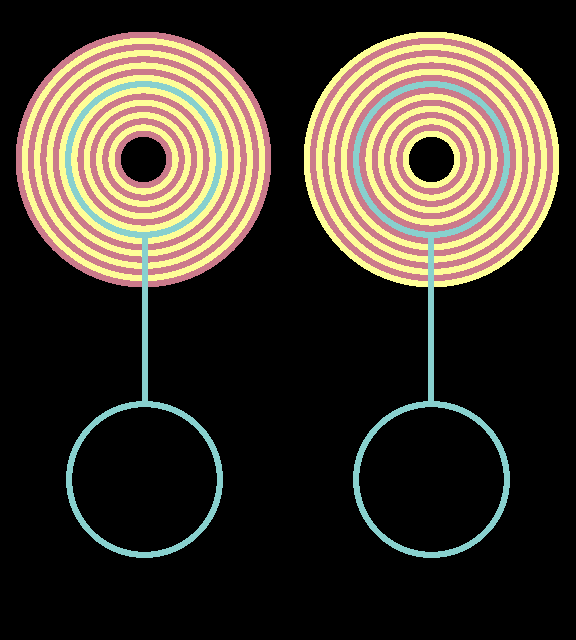
\includegraphics[width=0.5\textwidth]{test-circle-a-reference}
    \caption{Example of contextual influences on the perception of color. The colors of the rings on the left are physically identical to those on the right. The order of the rings differs, however. On the left, the 'green' ring is adjacent to two 'yellow' rings. On the right, the 'blue' ring is adjacent to two 'red' rings. This of context is what induces the perceived difference.}
    \label{fig:example}
\end{figure}

With these psychophysical observations in mind, much research has been devoted to elucidating the exact neurobiological mechanisms behind the perception of color, and the influence of context in it. The current view holds that while the LGN does indeed carry color and contrast information through separate pathways to V1, once there, the concepts of color and form become deeply intertwined as they are processed further. To explain this influence of form on color processing in V1, the literature proposes two broad classifications of neurons: single-opponent cells \& double-opponent cells \cite{johnson:2008}.

Opponency, in neurobiology, refers to antagonistic inputs of information: one source of input excites the neuron, while another inhibits it. These two antagonistic components of opponency are commonly referred to as the \textit{on} and \textit{off} inputs to a neuron. One can think of these two inputs as being what the cell is 'looking for', \textit{on}, and what the cell is 'not looking for', \textit{off}. Intuitively, stimuli from the \textit{on} input excites the neuron, while stimuli from the \textit{off} input inhibits it. Perhaps less intuitively, removal of stimuli from the \textit{off} input also excites the neuron. This behavior is logical when you consider that the two antagonistic inputs typically represent mutually exclusive features. In this way, removal of the negative stimuli often means much the same as presence of the positive stimuli and thus, removal of such stimuli contributes to excitation of the neuron. Of course, if equal stimuli are provided from both the \textit{on} and \textit{off} inputs, excitation is cancelled out by inhibition and the neuron does not fire. Lastly, recognize that any one neuron usually receives antagonistic input from, in fact, many other neurons. The aggregate stimuli from these excitatory and inhibitory inputs determines if the cell fires.

With respect to cells in the early visual system, we specifically use opponency to refer to chromatic and spatial opponency. We will now detail what exactly this means, with specific examples of neurons' expected patterns of response to various stimuli, as well as the implications of such responses. To frame this explanation, consider that single-opponent cells respond best to \textit{large areas} of light/color, while double-opponent cells respond only to the \textit{boundaries} between such areas.


\subsection*{Single-Opponent Neurons}

Single-opponent cells are a class of neurons in the early visual system which respond best to large areas of color and/or luminance. Their behavior is achieved by constructing classical center-surround receptive fields. The center receptive field serves as the \textit{on} input, exciting the cell when presented with a particular color, while the surround receptive field serves as the \textit{off} input, inhibiting the cell when another color is present or exciting it when that color is removed. These center and surround receptive fields may involve very few retinal cones, or may span many degrees of vision \cite{lennie:1991}.

In so called color preferring single-opponent cells, the cone inputs to the center and surround come from cones with different spectral response functions, e.g.: L vs M. By arranging input from different cones into antagonistic  receptive fields, we get a neuron which is sensitive to a particular color, in opposition to another. In the human visual system, we recognize three axes of such color opponency: redness vs. greenness, blueness vs. yellowness, and lightness vs. darkness. To construct these concepts of color, neurons in the visual pathway contrast activity of the three types of cone cells: those sensitive to long (L) wavelength light, those sensitive to medium (M) wavelength light, and those sensitive to short (S) wavelength light. By contrasting relative activity with neighboring L, M, and S cones, the retina itself can already begin to construct signal resembling psychological concepts of 'color'.

% FIGURE: Single-opponent receptive field schematics
\begin{figure}[H] \label{fig:so-rf-schematic}
    \centering
    \captionsetup{justification=centering}
    % 3 SUBFIGURES: Cross sections of single-opponent receptive fields
    \begin{subfigure}{0.3\textwidth}
        \centering
        \resizebox{\textwidth}{!}{%
        \begin{tikzpicture}
            % ON Center
            \draw[color=pomegranate!80, very thick] (-1.00, 0.00) .. controls (-0.30, 0.05) .. (-0.05, 2.00);
            \draw[color=pomegranate!80, very thick] (-0.05, 2.00) .. controls ( 0.00, 2.10) .. ( 0.05, 2.00);
            \draw[color=pomegranate!80, very thick] ( 1.00, 0.00) .. controls ( 0.30, 0.05) .. ( 0.05, 2.00)
                 node[color=black, anchor=south west] {$L^+$};
            % OFF Surround
            \draw[color=greensea,       very thick] (-1.00, 0.00) .. controls (-0.30,-0.05) .. (-0.05,-2.00);
            \draw[color=greensea,       very thick] (-0.05,-2.00) .. controls ( 0.00,-2.10) .. ( 0.05,-2.00);
            \draw[color=greensea,       very thick] ( 1.00, 0.00) .. controls ( 0.30,-0.05) .. ( 0.05,-2.00)
                 node[color=black, anchor=north west] {$M^-$};
            % Reference line & point
            \draw                                                             (-1.50, 0.00) -- ( 1.50, 0.00);
            \filldraw[color=black, fill=gray]                                 ( 0.00, 0.00) circle (2pt);
            % Frame to ensure alignment:
            \draw[color=white]                                                (-3.00, 2.50) rectangle (3.00, -2.50);
        \end{tikzpicture}}
    \end{subfigure}%
    \begin{subfigure}{0.3\textwidth}
        \centering
        \resizebox{\textwidth}{!}{%
        \begin{tikzpicture}
            % ON Center
            \draw[color=pomegranate!80, very thick] (-1.00, 0.00) .. controls (-0.30, 0.05) .. (-0.05, 2.00);
            \draw[color=pomegranate!80, very thick] (-0.05, 2.00) .. controls ( 0.00, 2.10) .. ( 0.05, 2.00);
            \draw[color=pomegranate!80, very thick] ( 1.00, 0.00) .. controls ( 0.30, 0.05) .. ( 0.05, 2.00)
                 node[color=black, anchor=south west] {$L^+$};
            % OFF Surround
            \draw[color=greensea,       very thick] (-1.00, 0.00) .. controls (-0.30,-0.05) .. (-0.05,-1.00);
            \draw[color=greensea,       very thick] (-0.05,-1.00) .. controls ( 0.00,-1.10) .. ( 0.05,-1.00);
            \draw[color=greensea,       very thick] ( 1.00, 0.00) .. controls ( 0.30,-0.05) .. ( 0.05,-1.00)
                 node[color=black, anchor=north west] {$M^-$};
            % Reference line & point
            \draw                                                             (-1.50, 0.00) -- ( 1.50, 0.00);
            \filldraw[color=black, fill=gray]                                 ( 0.00, 0.00) circle (2pt);
            % Frame to ensure alignment:
            \draw[color=white]                                                (-3.00, 2.50) rectangle (3.00, -2.50);
        \end{tikzpicture}}
    \end{subfigure}%
    \begin{subfigure}{0.3\textwidth}
        \centering
        \resizebox{\textwidth}{!}{%
        \begin{tikzpicture}
            % ON Center
            \draw[color=pomegranate!80, very thick] (-1.00, 0.00) .. controls (-0.30, 0.05) .. (-0.05, 2.00);
            \draw[color=pomegranate!80, very thick] (-0.05, 2.00) .. controls ( 0.00, 2.10) .. ( 0.05, 2.00);
            \draw[color=pomegranate!80, very thick] ( 1.00, 0.00) .. controls ( 0.30, 0.05) .. ( 0.05, 2.00)
                 node[color=black, anchor=south west] {$L^+$};
            % OFF Surround
            \draw[color=greensea,       very thick] (-1.50, 0.00) .. controls (-0.30,-0.20) .. (-0.05,-0.48);
            \draw[color=greensea,       very thick] (-0.05,-0.48) .. controls ( 0.00,-0.49) .. ( 0.05,-0.48);
            \draw[color=greensea,       very thick] ( 1.50, 0.00) .. controls ( 0.30,-0.20) .. ( 0.05,-0.48)
                 node[color=black, anchor=north west] {$M^-$};
            % Reference line & point
            \draw                                                             (-1.50, 0.00) -- ( 1.50, 0.00);
            \filldraw[color=black, fill=gray]                                 ( 0.00, 0.00) circle (2pt);
            % Frame to ensure alignment:
            \draw[color=white]                                                (-3.00, 2.50) rectangle (3.00, -2.50);
        \end{tikzpicture}}
    \end{subfigure}%
    \par \bigskip
    % 3 SUBFIGURES: Top-down view of single-opponent receptive fields
    \begin{subfigure}{0.3\textwidth}
        \centering
        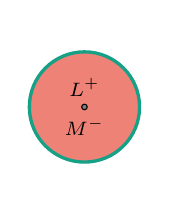
\begin{tikzpicture}
            % Frame to ensure alignment:
            \draw[color=white]                                         ( 0.00, -1.00) --     (0.00, 1.00);
            \filldraw[color=greensea,    fill=alizarin!70,  very thick]( 0.00,  0.00) circle (0.70)
                 node[color=black,       anchor=south] {$\scriptstyle L^+$}
                 node[color=black,       anchor=north] {$\scriptstyle M^-$};
            \filldraw[color=black,       fill=gray]                    ( 0.00,  0.00) circle (1pt);
        \end{tikzpicture}
        \caption{Symmetric \\ balanced \\ single-opponent \\ receptive field}
    \end{subfigure}%
    \begin{subfigure}{0.3\textwidth}
        \centering
        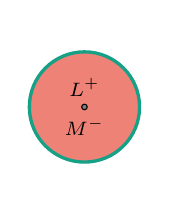
\begin{tikzpicture}
            % Frame to ensure alignment:
            \draw[color=white]                                         ( 0.00, -1.00) --     (0.00, 1.00);
            \filldraw[color=greensea,    fill=alizarin!70,  very thick]( 0.00,  0.00) circle (0.70)
                 node[color=black,       anchor=south] {$\scriptstyle L^+$}
                 node[color=black,       anchor=north] {$\scriptstyle M^-$};
            \filldraw[color=black,       fill=gray]                    ( 0.00,  0.00) circle (1pt);
        \end{tikzpicture}
        \caption{Symmetric \\ imbalanced \\ single-opponent \\ receptive field}
    \end{subfigure}%
    \begin{subfigure}{0.3\textwidth} \label{fig:so-rf-schematic-classic}
        \centering
        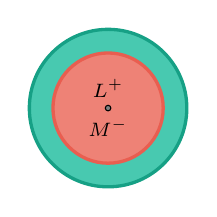
\begin{tikzpicture}
            \filldraw[color=greensea,    fill=turquoise!80, very thick]( 0.00,  0.00) circle (1.00);
            \filldraw[color=alizarin!90, fill=alizarin!70,  very thick]( 0.00,  0.00) circle (0.70)
                 node[color=black,       anchor=south] {$\scriptstyle L^+$}
                 node[color=black,       anchor=north] {$\scriptstyle M^-$};
            \filldraw[color=black,       fill=gray]                    ( 0.00,  0.00) circle (1pt);
        \end{tikzpicture}
        \caption{Classic \\ center/surround \\ single-opponent \\ receptive field}
    \end{subfigure}%
    \caption{Examples of possible single-opponent receptive field configurations, many others could be designed. All function to describe color properties of surfaces, though their response patterns to similar stimuli vary slightly.}
\end{figure}

As mentioned, one of the three axes of the opponent process theory is lightness vs. darkness. This is achieved in single-opponent cells by providing opponent inputs into the \textit{on} center and the \textit{off} surround from the same cones. By including input of L, M, and/or S cones into both the center and surround, the cells becomes 'color blind' and instead only respond to changes in luminosity. Sometimes incorrectly labeled as 'non-opponent', these neurons are, indeed, single-opponent cells: achromatic single-opponent cells.


\subsection*{Double-Opponent Neurons}

We have defined single-opponent cells to best respond to large areas of light/color. We now define double-opponent cells to respond only to the boundaries between such areas. In this regard, it is fair to think of double-opponent cells as biological 'edge detectors'. However, the precise definition of these cells is a topic of confusion in the field of neurobiology. All involved seem to agree that the input to the neuron is that of two single-opponent neurons itself. In this sense, the term "double-opponent" can be thought of as indicating that the dimensionality of color opponency has been doubled. However, another camp of researchers take the definition a step further and suggest that the two SO inputs are spatially offset. By this definition, the term "double-opponent" is thought to indicate that the cell is sensitive to opponency in two \textit{different} dimensions: color and space.

The distinction is non-trivial as the response patterns differ significantly, and thus the interpretation of their role in vision differs. Truly, both types of cells may, and likely do exist in the primate visual system [\textbf{//TODO} \textit{Cite studies which find these cells}]. However, for the purpose of our work we only consider the latter definition: double-opponent cells' receptive fields are both chromatically and spatially antagonistic.

\bigskip

\textbf{//TODO} \textbf{FIGURE: present the differences between the two DO configurations}

\bigskip

% FIGURE: Double-opponent receptive field schematics
\begin{figure}[H] \label{fig:do-rf-schematic}
    \centering
    \captionsetup{justification=centering}
    % 3 SUBFIGURES: Cross sections of double-opponent receptive fields
    \begin{subfigure}{0.3\textwidth}
        \centering
        \resizebox{\textwidth}{!}{%
        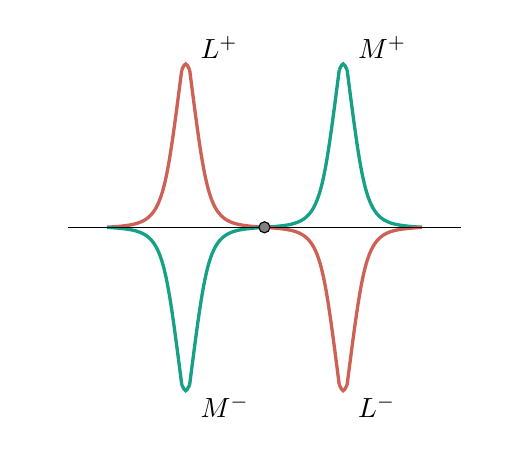
\begin{tikzpicture}
            % ON Center
            \draw[color=pomegranate!80, very thick] (-2.00, 0.00) .. controls (-1.30, 0.05) .. (-1.05, 2.00);
            \draw[color=pomegranate!80, very thick] (-1.05, 2.00) .. controls (-1.00, 2.10) .. (-0.95, 2.00);
            \draw[color=pomegranate!80, very thick] ( 0.00, 0.00) .. controls (-0.70, 0.05) .. (-0.95, 2.00)
                 node[color=black, anchor=south west] {$L^+$};
            % OFF Surround
            \draw[color=greensea,       very thick] (-2.00, 0.00) .. controls (-1.30,-0.05) .. (-1.05,-2.00);
            \draw[color=greensea,       very thick] (-1.05,-2.00) .. controls (-1.00,-2.10) .. (-0.95,-2.00);
            \draw[color=greensea,       very thick] ( 0.00, 0.00) .. controls (-0.70,-0.05) .. (-0.95,-2.00)
                 node[color=black, anchor=north west] {$M^-$};
            % ON Center
            \draw[color=greensea,       very thick] ( 0.00, 0.00) .. controls ( 0.70, 0.05) .. ( 0.95, 2.00);
            \draw[color=greensea,       very thick] ( 1.05, 2.00) .. controls ( 1.00, 2.10) .. ( 0.95, 2.00);
            \draw[color=greensea,       very thick] ( 2.00, 0.00) .. controls ( 1.30, 0.05) .. ( 1.05, 2.00)
                 node[color=black, anchor=south west] {$M^+$};
            % OFF Surround
            \draw[color=pomegranate!80, very thick] ( 0.00, 0.00) .. controls ( 0.70,-0.05) .. ( 0.95,-2.00);
            \draw[color=pomegranate!80, very thick] ( 1.05,-2.00) .. controls ( 1.00,-2.10) .. ( 0.95,-2.00);
            \draw[color=pomegranate!80, very thick] ( 2.00, 0.00) .. controls ( 1.30,-0.05) .. ( 1.05,-2.00)
                 node[color=black, anchor=north west] {$L^-$};
            % Reference line & point
            \draw                                                             (-2.50, 0.00) -- ( 2.50, 0.00);
            \filldraw[color=black, fill=gray]                                 ( 0.00, 0.00) circle (2pt);
            % Frame to ensure alignment:
            \draw[color=white]                                                (-3.00, 2.50) rectangle (3.00, -2.50);
        \end{tikzpicture}}
    \end{subfigure}
    \begin{subfigure}{0.3\textwidth}
        \resizebox{\textwidth}{!}{%
        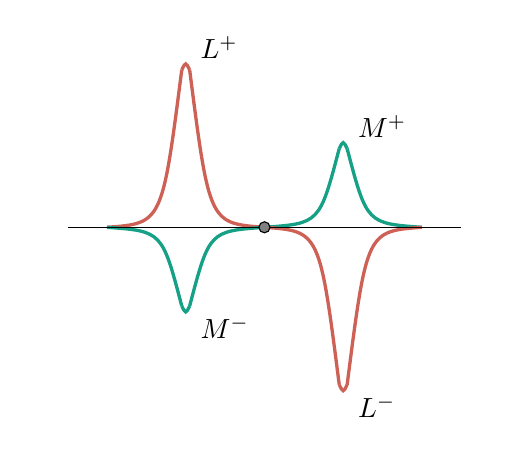
\begin{tikzpicture}
            % ON Center
            \draw[color=pomegranate!80, very thick] (-2.00, 0.00) .. controls (-1.30, 0.05) .. (-1.05, 2.00);
            \draw[color=pomegranate!80, very thick] (-1.05, 2.00) .. controls (-1.00, 2.10) .. (-0.95, 2.00);
            \draw[color=pomegranate!80, very thick] ( 0.00, 0.00) .. controls (-0.70, 0.05) .. (-0.95, 2.00)
                 node[color=black, anchor=south west] {$L^+$};
            % OFF Surround
            \draw[color=greensea,       very thick] (-2.00, 0.00) .. controls (-1.30,-0.05) .. (-1.05,-1.00);
            \draw[color=greensea,       very thick] (-1.05,-1.00) .. controls (-1.00,-1.10) .. (-0.95,-1.00);
            \draw[color=greensea,       very thick] ( 0.00, 0.00) .. controls (-0.70,-0.05) .. (-0.95,-1.00)
                 node[color=black, anchor=north west] {$M^-$};
            % ON Center
            \draw[color=greensea,       very thick] ( 0.00, 0.00) .. controls ( 0.70, 0.05) .. ( 0.95, 1.00);
            \draw[color=greensea,       very thick] ( 1.05, 1.00) .. controls ( 1.00, 1.10) .. ( 0.95, 1.00);
            \draw[color=greensea,       very thick] ( 2.00, 0.00) .. controls ( 1.30, 0.05) .. ( 1.05, 1.00)
                 node[color=black, anchor=south west] {$M^+$};
            % OFF Surround
            \draw[color=pomegranate!80, very thick] ( 0.00, 0.00) .. controls ( 0.70,-0.05) .. ( 0.95,-2.00);
            \draw[color=pomegranate!80, very thick] ( 1.05,-2.00) .. controls ( 1.00,-2.10) .. ( 0.95,-2.00);
            \draw[color=pomegranate!80, very thick] ( 2.00, 0.00) .. controls ( 1.30,-0.05) .. ( 1.05,-2.00)
                 node[color=black, anchor=north west] {$L^-$};
            % Reference line & point
            \draw                                                             (-2.50, 0.00) -- ( 2.50, 0.00);
            \filldraw[color=black, fill=gray]                                 ( 0.00, 0.00) circle (2pt);
            % Frame to ensure alignment:
            \draw[color=white]                                                (-3.00, 2.50) rectangle (3.00, -2.50);
        \end{tikzpicture}}
    \end{subfigure}
    \begin{subfigure}{0.3\textwidth}
        \resizebox{\textwidth}{!}{%
        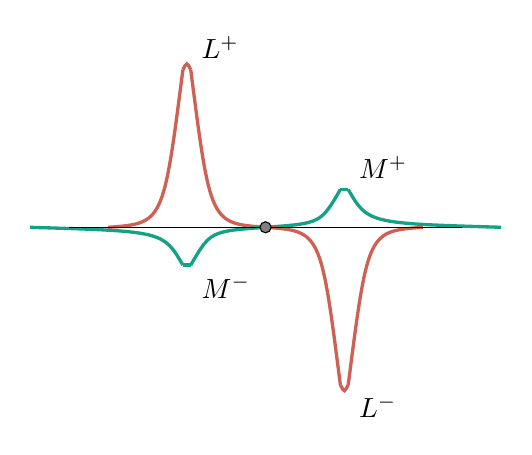
\begin{tikzpicture}
            % ON Center
            \draw[color=pomegranate!80, very thick] (-2.00, 0.00) .. controls (-1.30, 0.05) .. (-1.05, 2.00);
            \draw[color=pomegranate!80, very thick] (-1.05, 2.00) .. controls (-1.00, 2.10) .. (-0.95, 2.00);
            \draw[color=pomegranate!80, very thick] ( 0.00, 0.00) .. controls (-0.70, 0.05) .. (-0.95, 2.00)
                 node[color=black, anchor=south west] {$L^+$};
            % OFF Surround
            \draw[color=greensea,       very thick] (-3.00, 0.00) .. controls (-1.30,-0.05) .. (-1.05,-0.48);
            \draw[color=greensea,       very thick] (-1.05,-0.48) .. controls (-1.00,-0.49) .. (-0.95,-0.48);
            \draw[color=greensea,       very thick] ( 0.00, 0.00) .. controls (-0.70,-0.05) .. (-0.95,-0.48)
                 node[color=black, anchor=north west] {$M^-$};
            % ON Center
            \draw[color=greensea,       very thick] ( 0.00, 0.00) .. controls ( 0.70, 0.05) .. ( 0.95, 0.48);
            \draw[color=greensea,       very thick] ( 1.05, 0.48) .. controls ( 1.00, 0.49) .. ( 0.95, 0.48);
            \draw[color=greensea,       very thick] ( 3.00, 0.00) .. controls ( 1.30, 0.05) .. ( 1.05, 0.48)
                 node[color=black, anchor=south west] {$M^+$};
            % OFF Surround
            \draw[color=pomegranate!80, very thick] ( 0.00, 0.00) .. controls ( 0.70,-0.05) .. ( 0.95,-2.00);
            \draw[color=pomegranate!80, very thick] ( 1.05,-2.00) .. controls ( 1.00,-2.10) .. ( 0.95,-2.00);
            \draw[color=pomegranate!80, very thick] ( 2.00, 0.00) .. controls ( 1.30,-0.05) .. ( 1.05,-2.00)
                 node[color=black, anchor=north west] {$L^-$};
            % Reference line & point
            \draw                                                             (-2.50, 0.00) -- ( 2.50, 0.00);
            \filldraw[color=black, fill=gray]                                 ( 0.00, 0.00) circle (2pt);
            % Frame to ensure alignment:
            \draw[color=white]                                                (-3.00, 2.50) rectangle (3.00, -2.50);
        \end{tikzpicture}}
    \end{subfigure}%
    \par \bigskip
    % 3 SUBFIGURES: Top-down view of double-opponent receptive fields
    \begin{subfigure}{0.3\textwidth}
        \centering
        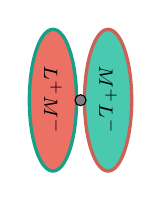
\begin{tikzpicture}
            \filldraw[color=pomegranate!80,       fill=turquoise!80, very thick]( 0.35, 0.00) ellipse   (0.30 and 0.90)
                 node[color=black, anchor=center, rotate=-90] {$\scriptstyle M^+L^-$};
            \filldraw[color=greensea, fill=alizarin!80,  very thick](-0.35, 0.00) ellipse   (0.30 and 0.90)
                 node[color=black, anchor=center, rotate=-90] {$\scriptstyle L^+M^-$};
            \filldraw[color=black,          fill=gray]                    ( 0.00, 0.00) circle    (2pt);
        \end{tikzpicture}
        \caption{Symmetric \\ balanced \\ double-opponent \\ receptive field}
    \end{subfigure}%
    \begin{subfigure}{0.3\textwidth}
        \centering
        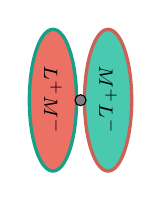
\begin{tikzpicture}
            \filldraw[color=pomegranate!80,       fill=turquoise!80, very thick]( 0.35, 0.00) ellipse   (0.30 and 0.90)
                 node[color=black, anchor=center, rotate=-90] {$\scriptstyle M^+L^-$};
            \filldraw[color=greensea, fill=alizarin!80,  very thick](-0.35, 0.00) ellipse   (0.30 and 0.90)
                 node[color=black, anchor=center, rotate=-90] {$\scriptstyle L^+M^-$};
            \filldraw[color=black,          fill=gray]                    ( 0.00, 0.00) circle    (2pt);
        \end{tikzpicture}
        \caption{Symmetric \\ imbalanced \\ double-opponent \\ receptive field}
    \end{subfigure}%
    \begin{subfigure}{0.3\textwidth} \label{fig:do-rf-schematic-classic}
        \centering
        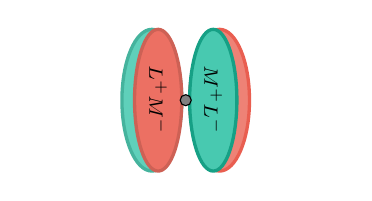
\begin{tikzpicture}
            % Frame to ensure alignment:
            \draw[color=white]                                            (-2.00, 0.00) --        (2.00, 0.00);
            \filldraw[color=alizarin!90,    fill=alizarin!70,  very thick]( 0.43, 0.00) ellipse   (0.38 and 0.90);
            \filldraw[color=greensea!80,    fill=turquoise!70, very thick](-0.43, 0.00) ellipse   (0.38 and 0.90);
            \filldraw[color=greensea,       fill=turquoise!80, very thick]( 0.35, 0.00) ellipse   (0.30 and 0.90)
                 node[color=black, anchor=center, rotate=-90] {$\scriptstyle M^+L^-$};
            \filldraw[color=pomegranate!80, fill=alizarin!80,  very thick](-0.35, 0.00) ellipse   (0.30 and 0.90)
                 node[color=black, anchor=center, rotate=-90] {$\scriptstyle L^+M^-$};
            \filldraw[color=black,          fill=gray]                    ( 0.00, 0.00) circle    (2pt);
        \end{tikzpicture}
        \caption{Center/ \\ surround \\ double-opponent \\ receptive field}
    \end{subfigure}%
    \caption{Examples of various possible double-opponent receptive field configurations, many others could be designed. All function to describe color properties of borders, though their response patterns to similar stimuli vary slightly.}
\end{figure}


\subsubsection*{Orientation Selectivity}

Research shows that cells identified as double-opponent tend to be orientation selective \cite{johnson:2008, sincich:2005, schluppeck:2002, chalupa:encyclopedia}. That is, they respond most strongly when stimulated by a border of particular orientation, less so with variation from that preferred orientation, and weekly, if at all, to borders orthogonal to the preferred orientation. This is intuitive given the organization of the receptive field as previously defined. By arranging the components of the receptive field to be spatially antagonistic, there will be one orientation of border which best separates the two components, and another orientation, precisely orthogonal, which does not separate the two components at all. This can be easily visualized, as in Figure \ref{fig:do-orient-h} and Figure \ref{fig:do-orient-v}.

It's worth noting that a single-opponent neuron can also be selective to specific orientations. These cells have been identified in biology, though their relative abundance appears minimal. To achieve orientation selectivity, the center and/or surround receptive fields simply need be made non-circular. However, without the balanced asymmetric \textit{on} and \textit{off} receptive fields from each opponent cone(s), an orientation specific single-opponent cell could never be as selective as a double-opponent cell.

% FIGURE: horizontal red/green double-opponent cell on horizontal red/green border
\afterpage{%
\begin{figure}[H] \label{fig:do-orient-h}
    \centering
    \begin{subfigure}{0.15\textwidth}
        \centering
        \resizebox{\textwidth}{!}{%
        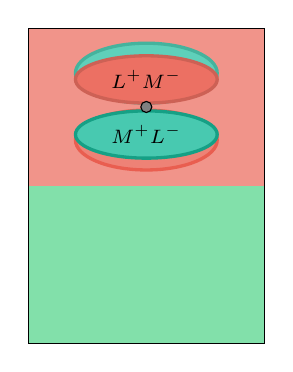
\begin{tikzpicture}
            \fill[alizarin!60]                                            (-1.50, 2.00) rectangle (1.50, 0.00);
            \fill[emerald!60]                                             (-1.50,-2.00) rectangle (1.50, 0.00);
            \filldraw[color=greensea!80,    fill=turquoise!70, very thick]( 0.00, 1.43) ellipse   (0.90 and 0.38);
            \filldraw[color=alizarin!90,    fill=alizarin!70,  very thick]( 0.00, 0.58) ellipse   (0.90 and 0.38);
            \filldraw[color=pomegranate!80, fill=alizarin!80,  very thick]( 0.00, 1.35) ellipse   (0.90 and 0.30)
                 node[color=black, anchor=center] {$\scriptstyle L^+M^-$};
            \filldraw[color=greensea,       fill=turquoise!80, very thick]( 0.00, 0.65) ellipse   (0.90 and 0.30)
                 node[color=black, anchor=center] {$\scriptstyle M^+L^-$};
            \filldraw[color=black,          fill=gray]                    ( 0.00, 1.00) circle    (2pt);
            \draw (current bounding box.north east) rectangle (current bounding box.south west);
        \end{tikzpicture}
        }
        \caption{Weak Response}
    \end{subfigure}%
    \begin{subfigure}{0.15\textwidth}
        \centering
        \resizebox{\textwidth}{!}{%
        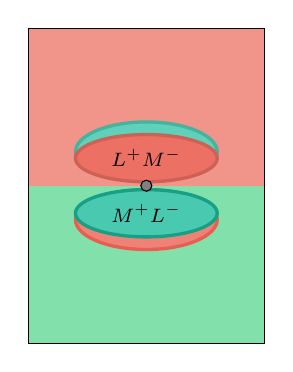
\begin{tikzpicture}
            \fill[alizarin!60]                                            (-1.50, 2.00) rectangle (1.50, 0.00);
            \fill[emerald!60]                                             (-1.50,-2.00) rectangle (1.50, 0.00);
            \filldraw[color=greensea!80,    fill=turquoise!70, very thick]( 0.00, 0.43) ellipse   (0.90 and 0.38);
            \filldraw[color=alizarin!90,    fill=alizarin!70,  very thick]( 0.00,-0.43) ellipse   (0.90 and 0.38);
            \filldraw[color=pomegranate!80, fill=alizarin!80,  very thick]( 0.00, 0.35) ellipse   (0.90 and 0.30)
                 node[color=black, anchor=center] {$\scriptstyle L^+M^-$};
            \filldraw[color=greensea,       fill=turquoise!80, very thick]( 0.00,-0.35) ellipse   (0.90 and 0.30)
                 node[color=black, anchor=center] {$\scriptstyle M^+L^-$};
            \filldraw[color=black,          fill=gray]                    ( 0.00, 0.00) circle    (2pt);
        \draw (current bounding box.north east) rectangle (current bounding box.south west);
        \end{tikzpicture}
        }
        \caption{Stong Response}
    \end{subfigure}%
    \begin{subfigure}{0.15\textwidth}
        \centering
        \resizebox{\textwidth}{!}{%
        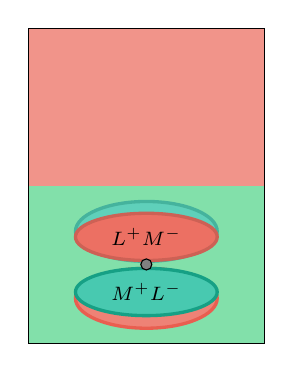
\begin{tikzpicture}
            \fill[alizarin!60]                                            (-1.50, 2.00) rectangle (1.50, 0.00);
            \fill[emerald!60]                                             (-1.50,-2.00) rectangle (1.50, 0.00);
            \filldraw[color=greensea!80,    fill=turquoise!70, very thick]( 0.00,-0.58) ellipse   (0.90 and 0.38);
            \filldraw[color=alizarin!90,    fill=alizarin!70,  very thick]( 0.00,-1.43) ellipse   (0.90 and 0.38);
            \filldraw[color=pomegranate!80, fill=alizarin!80,  very thick]( 0.00,-0.65) ellipse   (0.90 and 0.30)
                 node[color=black, anchor=center] {$\scriptstyle L^+M^-$};
            \filldraw[color=greensea,       fill=turquoise!80, very thick]( 0.00,-1.35) ellipse   (0.90 and 0.30)
                 node[color=black, anchor=center] {$\scriptstyle M^+L^-$};
            \filldraw[color=black,          fill=gray]                    ( 0.00,-1.00) circle    (2pt);
        \draw (current bounding box.north east) rectangle (current bounding box.south west);
        \end{tikzpicture}
        }
        \caption{Weak Response}
    \end{subfigure}%
    \par \bigskip
    \begin{subfigure}{0.15\textwidth}
        \centering
        \resizebox{\textwidth}{!}{%
        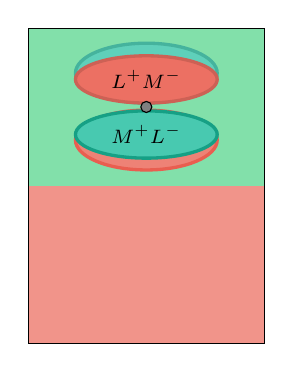
\begin{tikzpicture}
            \fill[emerald!60]                                             (-1.50, 2.00) rectangle (1.50, 0.00);
            \fill[alizarin!60]                                            (-1.50,-2.00) rectangle (1.50, 0.00);
            \filldraw[color=greensea!80,    fill=turquoise!70, very thick]( 0.00, 1.43) ellipse   (0.90 and 0.38);
            \filldraw[color=alizarin!90,    fill=alizarin!70,  very thick]( 0.00, 0.58) ellipse   (0.90 and 0.38);
            \filldraw[color=pomegranate!80, fill=alizarin!80,  very thick]( 0.00, 1.35) ellipse   (0.90 and 0.30)
                 node[color=black, anchor=center] {$\scriptstyle L^+M^-$};
            \filldraw[color=greensea,       fill=turquoise!80, very thick]( 0.00, 0.65) ellipse   (0.90 and 0.30)
                 node[color=black, anchor=center] {$\scriptstyle M^+L^-$};
            \filldraw[color=black,          fill=gray]                    ( 0.00, 1.00) circle    (2pt);
            \draw (current bounding box.north east) rectangle (current bounding box.south west);
        \end{tikzpicture}
        }
        \caption{Weak Response}
    \end{subfigure}%
    \begin{subfigure}{0.15\textwidth}
        \centering
        \resizebox{\textwidth}{!}{%
        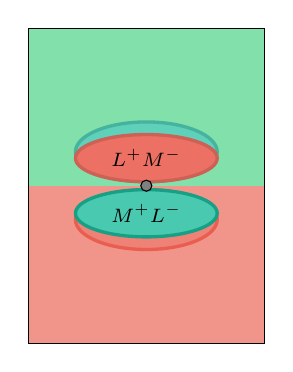
\begin{tikzpicture}
            \fill[emerald!60]                                             (-1.50, 2.00) rectangle (1.50, 0.00);
            \fill[alizarin!60]                                            (-1.50,-2.00) rectangle (1.50, 0.00);
            \filldraw[color=greensea!80,    fill=turquoise!70, very thick]( 0.00, 0.43) ellipse   (0.90 and 0.38);
            \filldraw[color=alizarin!90,    fill=alizarin!70,  very thick]( 0.00,-0.43) ellipse   (0.90 and 0.38);
            \filldraw[color=pomegranate!80, fill=alizarin!80,  very thick]( 0.00, 0.35) ellipse   (0.90 and 0.30)
                 node[color=black, anchor=center] {$\scriptstyle L^+M^-$};
            \filldraw[color=greensea,       fill=turquoise!80, very thick]( 0.00,-0.35) ellipse   (0.90 and 0.30)
                 node[color=black, anchor=center] {$\scriptstyle M^+L^-$};
            \filldraw[color=black,          fill=gray]                    ( 0.00, 0.00) circle    (2pt);
        \draw (current bounding box.north east) rectangle (current bounding box.south west);
        \end{tikzpicture}
        }
        \caption{No Response}
    \end{subfigure}%
    \begin{subfigure}{0.15\textwidth}
        \centering
        \resizebox{\textwidth}{!}{%
        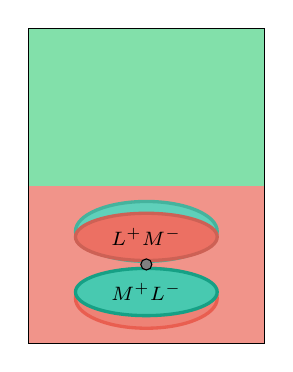
\begin{tikzpicture}
            \fill[emerald!60]                                             (-1.50, 2.00) rectangle (1.50, 0.00);
            \fill[alizarin!60]                                            (-1.50,-2.00) rectangle (1.50, 0.00);
            \filldraw[color=greensea!80,    fill=turquoise!70, very thick]( 0.00,-0.58) ellipse   (0.90 and 0.38);
            \filldraw[color=alizarin!90,    fill=alizarin!70,  very thick]( 0.00,-1.43) ellipse   (0.90 and 0.38);
            \filldraw[color=pomegranate!80, fill=alizarin!80,  very thick]( 0.00,-0.65) ellipse   (0.90 and 0.30)
                 node[color=black, anchor=center] {$\scriptstyle L^+M^-$};
            \filldraw[color=greensea,       fill=turquoise!80, very thick]( 0.00,-1.35) ellipse   (0.90 and 0.30)
                 node[color=black, anchor=center] {$\scriptstyle M^+L^-$};
            \filldraw[color=black,          fill=gray]                    ( 0.00,-1.00) circle    (2pt);
        \draw (current bounding box.north east) rectangle (current bounding box.south west);
        \end{tikzpicture}
        }
        \caption{Weak Response}
    \end{subfigure}
    \caption{A double opponent cell selective to horizontally oriented borders with red above and green below; only responsive to that particular stimulus. In Figure (b), the neuron is presented with its ideal stimulus: its $L^+$ and $M^+$ receptive fields are fully activated while its $L^-$ and $M^-$ receptive fields are completely unactivated. Figure (e) presents the neuron with the exact opposite stimulus, neither its $L^+$ nor $M^+$ receptive fields are activate at all, and both its $L^-$ and $M^-$ receptive fields are fully activated, ensuring no response possible from the cell. While its $L^+$ receptive field might be strongly stimulated in (a) and (f), it's $L^-$ receptive field cancels it out. Similarly, in (c) and (d) its $M^+$ receptive field is stimulated but cancelled out by activity in its $M^-$ receptive field.}
\end{figure}
% FIGURE: vertical red/green double-opponent cell on horizontal red/green border
\begin{figure}[H] \label{fig:do-orient-v}
    \centering
    \begin{subfigure}{0.15\textwidth}
        \centering
        \resizebox{\textwidth}{!}{%
        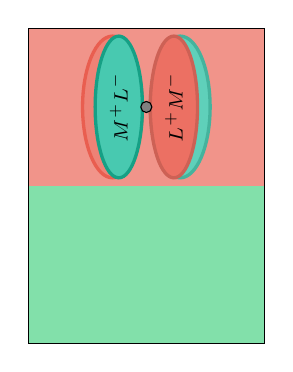
\begin{tikzpicture}
            \fill[alizarin!60]                                            (-1.50, 2.00) rectangle (1.50, 0.00);
            \fill[emerald!60]                                             (-1.50,-2.00) rectangle (1.50, 0.00);
            \filldraw[color=greensea!80,    fill=turquoise!70, very thick]( 0.43, 1.00) ellipse   (0.38 and 0.90);
            \filldraw[color=alizarin!90,    fill=alizarin!70,  very thick](-0.43, 1.00) ellipse   (0.38 and 0.90);
            \filldraw[color=pomegranate!80, fill=alizarin!80,  very thick]( 0.35, 1.00) ellipse   (0.30 and 0.90)
                 node[color=black, anchor=center, rotate=90] {$\scriptstyle L^+M^-$};
            \filldraw[color=greensea,       fill=turquoise!80, very thick](-0.35, 1.00) ellipse   (0.30 and 0.90)
                 node[color=black, anchor=center, rotate=90] {$\scriptstyle M^+L^-$};
            \filldraw[color=black,          fill=gray]                    ( 0.00, 1.00) circle    (2pt);
            \draw (current bounding box.north east) rectangle (current bounding box.south west);
        \end{tikzpicture}
        }
        \caption{Weak Response}
    \end{subfigure}%
    \begin{subfigure}{0.15\textwidth}
        \centering
        \resizebox{\textwidth}{!}{%
        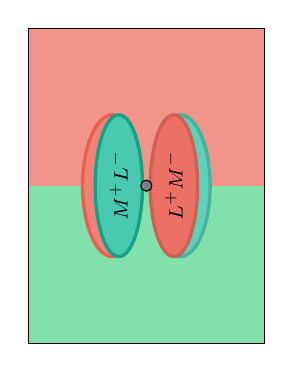
\begin{tikzpicture}
            \fill[alizarin!60]                                            (-1.50, 2.00) rectangle (1.50, 0.00);
            \fill[emerald!60]                                             (-1.50,-2.00) rectangle (1.50, 0.00);
            \filldraw[color=greensea!80,    fill=turquoise!70, very thick]( 0.43, 0.00) ellipse   (0.38 and 0.90);
            \filldraw[color=alizarin!90,    fill=alizarin!70,  very thick](-0.43, 0.00) ellipse   (0.38 and 0.90);
            \filldraw[color=pomegranate!80, fill=alizarin!80,  very thick]( 0.35, 0.00) ellipse   (0.30 and 0.90)
                 node[color=black, anchor=center, rotate=90] {$\scriptstyle L^+M^-$};
            \filldraw[color=greensea,       fill=turquoise!80, very thick](-0.35, 0.00) ellipse   (0.30 and 0.90)
                 node[color=black, anchor=center, rotate=90] {$\scriptstyle M^+L^-$};
            \filldraw[color=black,          fill=gray]                    ( 0.00, 0.00) circle    (2pt);
            \draw (current bounding box.north east) rectangle (current bounding box.south west);
        \end{tikzpicture}
        }
        \caption{Weak Response}
    \end{subfigure}%
    \begin{subfigure}{0.15\textwidth}
        \centering
        \resizebox{\textwidth}{!}{%
        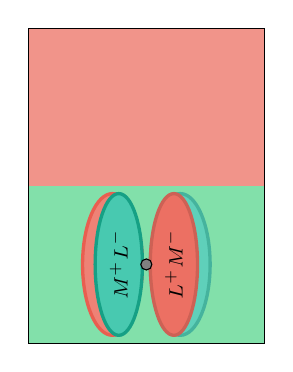
\begin{tikzpicture}
            \fill[alizarin!60]                                            (-1.50, 2.00) rectangle (1.50, 0.00);
            \fill[emerald!60]                                             (-1.50,-2.00) rectangle (1.50, 0.00);
            \filldraw[color=greensea!80,    fill=turquoise!70, very thick]( 0.43,-1.00) ellipse   (0.38 and 0.90);
            \filldraw[color=alizarin!90,    fill=alizarin!70,  very thick](-0.43,-1.00) ellipse   (0.38 and 0.90);
            \filldraw[color=pomegranate!80, fill=alizarin!80,  very thick]( 0.35,-1.00) ellipse   (0.30 and 0.90)
                 node[color=black, anchor=center, rotate=90] {$\scriptstyle L^+M^-$};
            \filldraw[color=greensea,       fill=turquoise!80, very thick](-0.35,-1.00) ellipse   (0.30 and 0.90)
                 node[color=black, anchor=center, rotate=90] {$\scriptstyle M^+L^-$};
            \filldraw[color=black,          fill=gray]                    ( 0.00,-1.00) circle    (2pt);
            \draw (current bounding box.north east) rectangle (current bounding box.south west);
        \end{tikzpicture}
        }
        \caption{Weak Response}
    \end{subfigure}%
    \par \bigskip
    \begin{subfigure}{0.15\textwidth}
        \centering
        \resizebox{\textwidth}{!}{%
        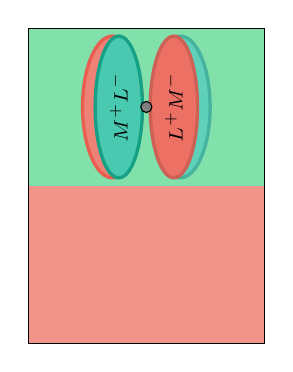
\begin{tikzpicture}
            \fill[emerald!60]                                             (-1.50, 2.00) rectangle (1.50, 0.00);
            \fill[alizarin!60]                                            (-1.50,-2.00) rectangle (1.50, 0.00);
            \filldraw[color=greensea!80,    fill=turquoise!70, very thick]( 0.43, 1.00) ellipse   (0.38 and 0.90);
            \filldraw[color=alizarin!90,    fill=alizarin!70,  very thick](-0.43, 1.00) ellipse   (0.38 and 0.90);
            \filldraw[color=pomegranate!80, fill=alizarin!80,  very thick]( 0.35, 1.00) ellipse   (0.30 and 0.90)
                 node[color=black, anchor=center, rotate=90] {$\scriptstyle L^+M^-$};
            \filldraw[color=greensea,       fill=turquoise!80, very thick](-0.35, 1.00) ellipse   (0.30 and 0.90)
                 node[color=black, anchor=center, rotate=90] {$\scriptstyle M^+L^-$};
            \filldraw[color=black,          fill=gray]                    ( 0.00, 1.00) circle    (2pt);
            \draw (current bounding box.north east) rectangle (current bounding box.south west);
        \end{tikzpicture}
        }
        \caption{Weak Response}
    \end{subfigure}%
    \begin{subfigure}{0.15\textwidth}
        \centering
        \resizebox{\textwidth}{!}{%
        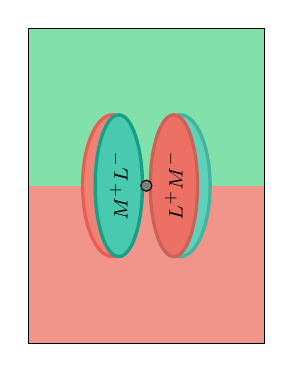
\begin{tikzpicture}
            \fill[emerald!60]                                             (-1.50, 2.00) rectangle (1.50, 0.00);
            \fill[alizarin!60]                                            (-1.50,-2.00) rectangle (1.50, 0.00);
            \filldraw[color=greensea!80,    fill=turquoise!70, very thick]( 0.43, 0.00) ellipse   (0.38 and 0.90);
            \filldraw[color=alizarin!90,    fill=alizarin!70,  very thick](-0.43, 0.00) ellipse   (0.38 and 0.90);
            \filldraw[color=pomegranate!80, fill=alizarin!80,  very thick]( 0.35, 0.00) ellipse   (0.30 and 0.90)
                 node[color=black, anchor=center, rotate=90] {$\scriptstyle L^+M^-$};
            \filldraw[color=greensea,       fill=turquoise!80, very thick](-0.35, 0.00) ellipse   (0.30 and 0.90)
                 node[color=black, anchor=center, rotate=90] {$\scriptstyle M^+L^-$};
            \filldraw[color=black,          fill=gray]                    ( 0.00, 0.00) circle    (2pt);
            \draw (current bounding box.north east) rectangle (current bounding box.south west);
        \end{tikzpicture}
        }
        \caption{Weak Response}
    \end{subfigure}%
    \begin{subfigure}{0.15\textwidth}
        \centering
        \resizebox{\textwidth}{!}{%
        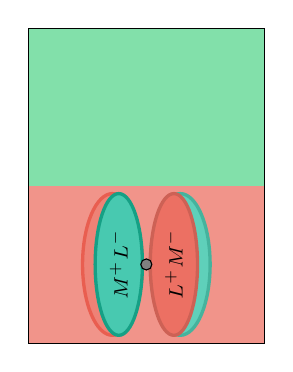
\begin{tikzpicture}
            \fill[emerald!60]                                             (-1.50, 2.00) rectangle (1.50, 0.00);
            \fill[alizarin!60]                                            (-1.50,-2.00) rectangle (1.50, 0.00);
            \filldraw[color=greensea!80,    fill=turquoise!70, very thick]( 0.43,-1.00) ellipse   (0.38 and 0.90);
            \filldraw[color=alizarin!90,    fill=alizarin!70,  very thick](-0.43,-1.00) ellipse   (0.38 and 0.90);
            \filldraw[color=pomegranate!80, fill=alizarin!80,  very thick]( 0.35,-1.00) ellipse   (0.30 and 0.90)
                 node[color=black, anchor=center, rotate=90] {$\scriptstyle L^+M^-$};
            \filldraw[color=greensea,       fill=turquoise!80, very thick](-0.35,-1.00) ellipse   (0.30 and 0.90)
                 node[color=black, anchor=center, rotate=90] {$\scriptstyle M^+L^-$};
            \filldraw[color=black,          fill=gray]                    ( 0.00,-1.00) circle    (2pt);
            \draw (current bounding box.north east) rectangle (current bounding box.south west);
        \end{tikzpicture}
        }
        \caption{Weak Response}
    \end{subfigure}
    \caption{A double opponent cell selective to vertically oriented borders with red to the right and green on the left; completely unresponsive to a horizontal border. While its $L^+$ receptive field might be strongly stimulated in (a) and (f), it's $L^-$ receptive field cancels it out. Similarly, in (c) and (d) its $M^+$ receptive field is stimulated but cancelled out by activity in its $M^-$ receptive field. In (b) and (e) both of its $L^+$ and $M^+$ receptive fields are moderately activated, but again, cancelled out by activation in its $L^-$ and $M^-$ receptive fields, respectively.}
\end{figure}
\clearpage
}

\subsubsection*{Spatial Frequency Selectivity}

Another important feature of double-opponent cells is that they are inherently sensitive to borders of specific size, or scale. Technically, we refer to such preference of 'scale' as a cell's spatial frequency selectivity. Each double-opponent neuron will be selective to a particular spatial frequency and excited less so by stimuli of spatial frequency deviating from this preference. Again, this is quite intuitively a product of the design of the neuron's receptive field and easily visualized, as in Figure \ref{fig:do-scale}.

% FIGURE: horizontal red/green double-opponent cell on horizontal red/green border of different spatial frequencies
\begin{figure}[h]
    \centering
    \begin{subfigure}{0.2\textwidth}
        \centering
        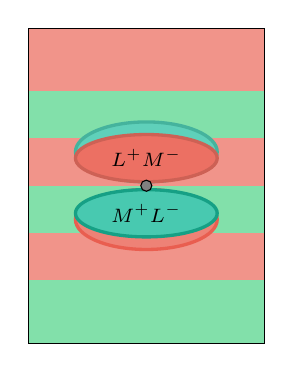
\begin{tikzpicture}
            \fill[alizarin!60]                                            (-1.50, 2.00) rectangle (1.50, 1.20);
            \fill[emerald!60]                                             (-1.50, 1.20) rectangle (1.50, 0.60);
            \fill[alizarin!60]                                            (-1.50, 0.60) rectangle (1.50, 0.00);
            \fill[emerald!60]                                             (-1.50,-0.60) rectangle (1.50, 0.00);
            \fill[alizarin!60]                                            (-1.50,-1.20) rectangle (1.50,-0.60);
            \fill[emerald!60]                                             (-1.50,-2.00) rectangle (1.50,-1.20);
            \filldraw[color=greensea!80,    fill=turquoise!70, very thick]( 0.00, 0.43) ellipse   (0.90 and 0.38);
            \filldraw[color=alizarin!90,    fill=alizarin!70,  very thick]( 0.00,-0.43) ellipse   (0.90 and 0.38);
            \filldraw[color=pomegranate!80, fill=alizarin!80,  very thick]( 0.00, 0.35) ellipse   (0.90 and 0.30)
                 node[color=black, anchor=center] {$\scriptstyle L^+M^-$};
            \filldraw[color=greensea,       fill=turquoise!80, very thick]( 0.00,-0.35) ellipse   (0.90 and 0.30)
                 node[color=black, anchor=center] {$\scriptstyle M^+L^-$};
            \filldraw[color=black,          fill=gray]                    ( 0.00, 0.00) circle    (2pt);
        \draw (current bounding box.north east) rectangle (current bounding box.south west);
        \end{tikzpicture}
        \caption{Maximum Response}
    \end{subfigure}%
    \begin{subfigure}{0.2\textwidth}
        \centering
        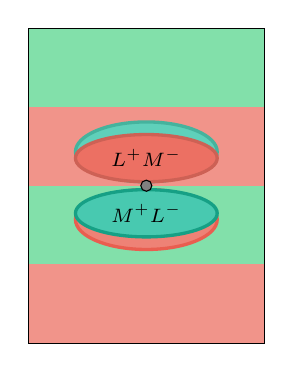
\begin{tikzpicture}
            \fill[emerald!60]                                             (-1.50, 2.00) rectangle (1.50, 1.00);
            \fill[alizarin!60]                                            (-1.50, 1.00) rectangle (1.50, 0.00);
            \fill[emerald!60]                                             (-1.50,-1.00) rectangle (1.50, 0.00);
            \fill[alizarin!60]                                            (-1.50,-2.00) rectangle (1.50,-1.00);
            \filldraw[color=greensea!80,    fill=turquoise!70, very thick]( 0.00, 0.43) ellipse   (0.90 and 0.38);
            \filldraw[color=alizarin!90,    fill=alizarin!70,  very thick]( 0.00,-0.43) ellipse   (0.90 and 0.38);
            \filldraw[color=pomegranate!80, fill=alizarin!80,  very thick]( 0.00, 0.35) ellipse   (0.90 and 0.30)
                 node[color=black, anchor=center] {$\scriptstyle L^+M^-$};
            \filldraw[color=greensea,       fill=turquoise!80, very thick]( 0.00,-0.35) ellipse   (0.90 and 0.30)
                 node[color=black, anchor=center] {$\scriptstyle M^+L^-$};
            \filldraw[color=black,          fill=gray]                    ( 0.00, 0.00) circle    (2pt);
        \draw (current bounding box.north east) rectangle (current bounding box.south west);
        \end{tikzpicture}
        \caption{Maximum Response}
    \end{subfigure}%
    \begin{subfigure}{0.2\textwidth}
        \centering
        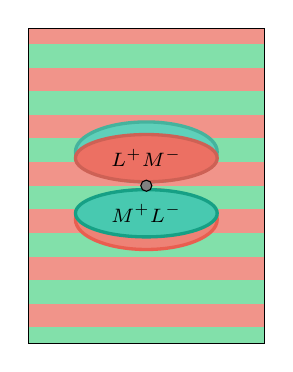
\begin{tikzpicture}
            \fill[alizarin!60]                                            (-1.50, 2.00) rectangle (1.50, 1.80);
            \fill[emerald!60]                                             (-1.50, 1.80) rectangle (1.50, 1.50);
            \fill[alizarin!60]                                            (-1.50, 1.50) rectangle (1.50, 1.20);
            \fill[emerald!60]                                             (-1.50, 1.20) rectangle (1.50, 0.90);
            \fill[alizarin!60]                                            (-1.50, 0.90) rectangle (1.50, 0.60);
            \fill[emerald!60]                                             (-1.50, 0.60) rectangle (1.50, 0.30);
            \fill[alizarin!60]                                            (-1.50, 0.30) rectangle (1.50, 0.00);
            \fill[emerald!60]                                             (-1.50,-0.30) rectangle (1.50, 0.00);
            \fill[alizarin!60]                                            (-1.50,-0.60) rectangle (1.50,-0.30);
            \fill[emerald!60]                                             (-1.50,-0.90) rectangle (1.50,-0.60);
            \fill[alizarin!60]                                            (-1.50,-1.20) rectangle (1.50,-0.90);
            \fill[emerald!60]                                             (-1.50,-1.50) rectangle (1.50,-1.20);
            \fill[alizarin!60]                                            (-1.50,-1.80) rectangle (1.50,-1.50);
            \fill[emerald!60]                                             (-1.50,-2.00) rectangle (1.50,-1.80);
            \filldraw[color=greensea!80,    fill=turquoise!70, very thick]( 0.00, 0.43) ellipse   (0.90 and 0.38);
            \filldraw[color=alizarin!90,    fill=alizarin!70,  very thick]( 0.00,-0.43) ellipse   (0.90 and 0.38);
            \filldraw[color=pomegranate!80, fill=alizarin!80,  very thick]( 0.00, 0.35) ellipse   (0.90 and 0.30)
                 node[color=black, anchor=center] {$\scriptstyle L^+M^-$};
            \filldraw[color=greensea,       fill=turquoise!80, very thick]( 0.00,-0.35) ellipse   (0.90 and 0.30)
                 node[color=black, anchor=center] {$\scriptstyle M^+L^-$};
            \filldraw[color=black,          fill=gray]                    ( 0.00, 0.00) circle    (2pt);
        \draw (current bounding box.north east) rectangle (current bounding box.south west);
        \end{tikzpicture}
        \caption{Maximum Response}
    \end{subfigure}%
    \caption{A double opponent cell tuned to a particular spatial frequency. Either a (b) lower or a (c) higher spatial frequency than preferred lowers the response of the cell.} \label{fig:do-scale}
\end{figure}

\bigskip

\textbf{//TODO} \textit{CONTRAST WITH SINGLE-OPPONENT'S LACK OF SPATIAL FREQ. SELECTIVITY (show Shapley's graphs)}

\textit{[erm.. don't we have spatial frequency for SO also??]}

\bigskip

\subsubsection*{Achromatic Double-Opponent Neurons}

As with single-opponent cells, one of the axes of the opponent process theory is 'lightness' vs 'darkness'. While we frequently discuss opponency as being a thing of 'color', we find double-opponent cells which are specifically sensitive to luminance borders.
Such achromatic sensitivity is easily achieved by balancing cone inputs into the neuron's antagonistic receptive fields, as in single-opponent cells. It behaves just as the previously described double-opponent cells, with specific orientation and spatial frequency selectivity, but responds best to luminosity borders rather than chromatic borders. For more details on achromatic receptive fields, please refer back to the section on \textit{Achromatic Single-Opponent Neurons}.
It is important to reiterate here that the \textit{on} and \textit{off} inputs to light and dark sensitive single-opponent cells are balanced, whereas their chromatic sensitive counterparts are imbalanced in inputs (\textbf{//TODO} \textit{incorrect terminology, we use 'imbalanced' differently in SO graphics}). This has the implication at the double-opponent level that light and dark double-opponent cells are redundant, as can be seen in Figures \ref{fig:do-rf-inputs-light} and \ref{fig:do-rf-inputs-dark}. This is in contrast to the chromatic double-opponent cells depictied in Figure \ref{fig:do-rf-inputs} which differentiate themselves from their opponent pair by imbalanced inputs from the same cones.


\subsection*{Hypercolumns}

Thus far we have defined two broad classes of neurons in the primate visual system: single-opponent and double-opponent. Each class has a number of parameters which dictate what stimuli the cell should respond to: opponent color, orientation selectivity, and spatial frequency. A single cell can only be sensitive to a specific combination of settings for each parameter. However, for each parameter it is important to have neurons sensitive to the full range of parameters. Thus, it is necessary to have a collection of neurons which together cover the complete combinatorial set of settings for all parameters.

Furthermore, as may be obvious, the receptive field of a neuron in V1 is directly \textbf{connected/related/tied \textit{(???)}} to a set of neurons in the retina. That is, neurons in V1 are sensitive only to activity at a particular physical location on the retina; V1 is \textit{retinotopic}, or retinally mapped.

The implication is that for each retinal position, in V1 it is necessary to have a large number of both single-opponent and double-opponent cells, selective to the full gamut of parameters possible for each type of cell. Biologically, these collections of cells are organized in \textit{hypercolumns}, a physical grouping of cells in which neuronal connections 'up' and 'down' within the column are much more dense than extensions to cells in other columns. Within a single hypercolumn, all cells are sensitive to a specific retinal location, but together express sensitivity to the full range of parameters.


\subsection{Computational Modeling:}

The model described in this research is an extension of that presented by Penacchio \textit{et al.} \cite{otazu:plosive}, itself based on work by Z. Li \cite{li:1998, li:1999}. Before detailing our implementation, it is important to review prior art; these works and others. As our goal is to model the behavior of color preferring and achromatic single-opponent and double-opponent neurons, we will also review other computational endeavors tackling the issue of color and/or form from a biologically inspired perspective.

\subsection*{Li's Neurodynamical Model for Segmentation (1999)}
In Li's original work, a neurodynamical model was presented which focused on global region segmentation using only local interactions between neurons. In the interest of simplicity, Li's implementation dealt only with the nature of these interactions, ignoring where the stimulus, or information, might be coming from. Conceptually, Li defined neurons by their physical position in the image and the 'feature' to which they are sensitive. She then defined the connections between these neurons such that those physically close to each other, and sensitive to similar features, interacted most strongly. Stimulation of one neuron, then, positively stimulated (excited) similar neurons nearby, and negatively stimulated (inhibited) dissimilar neurons nearby. Such excitation and inhibition cascades through the network naturally, producing large scale response patterns defined only by local stimuli.

In the model presented, Li used oriented bars as features, though expressed that any logical feature could be reasonably considered in its place. This choice was biologically inspired by neurons sensitive to specifically oriented bars, the aforementioned double-opponent cells. When considering such features, inter-neuronal connections can be logically deduced: two neurons positively interact most when both 1) are sensitive to similarly oriented bars and 2) are co-located along that same orientation. Two neurons negatively interact most when either of these two conditions is not met.

By defining neuronal connectivity in this manner, patterns of neurons sensitive to co-located and co-aligned bars positively interact with each other to enhance their collective response to the stimuli. Similarly, incoherent stimuli negatively interact with their neighbors and are silenced. From these local interactions, global features are enhanced if they satisfy the connectivity rules, and noise is suppressed. Li showed that this method can be used to enhance contours and identify boundaries between regions for which normal segmentation methods struggle.


\subsection*{Penacchio, Otazu, \& Dempere-Marco's Neurodynamical Model for Brightness Induction (2013)}

Li's work laid the foundation for Penacchio \textit{et al.} who extended the model to a usable framework which:
\begin{enumerate}
    \item Uses real black \& white images /movies as input.
    \item Utilizes discrete wavelet transforms to extract edges (more on this later).
    \item Added multi scale support.
    \item Summarizes the results into an output 'perceptual image'.
\end{enumerate}
Their research was focused on observing brightness induction (BI) arising from such a neurodynamical model.
\begin{itemize}
    \item No color, just black \& white \textit{edges}
    \item Generalized to real images (edges vs lines)
    \item Added scales
    \item Dynamical processing
    \item \textbf{Avoid detail, save that for \textit{Method}..?}
    \item Extension of Z. Li's edge detection work
    \item Uses DWT to extract oriented edges in grayscale
    \begin{itemize}
        \item ..in our context, it's essentially a luminance sensitive double-opponent cell.
    \end{itemize}
\end{itemize}

\subsection*{Itti, Koch, \& Niebur's Model for Saliency \cite{itti:1998}}

Itti \textit{et al.} implemented a biologically inspired model of visual attention, or saliency. This work included opponent processing of color, center/surround receptive fields at scales, and orientation selectivity. Because of these features, and their overlap with our own goals, we consider it an important work to consider.

Color is included in this model by treating the color channels of the RGB image as analogous for L, M, and S cone activity. From this, red, green, blue, and yellow color components, as well as a single intensity components are derived, using the following formulae:

\begin{flalign}
    I &= \frac{(r + g + b)}{3} \\
    R &= max(0, r - \frac{(g + b)}{2}) \\
    G &= max(0, g - \frac{(r + b)}{2}) \\
    B &= max(0, b - \frac{(r + g)}{2}) \\
    Y &= max(0, \frac{(r + g)}{2} - \frac{|(r + g)|}{2} - b)
\end{flalign}

Each of the $r$, $g$, and $b$ channels are normalized by $I$ in order to decouple hue from intensity.

These derived color components (and intensity) are computed for a set of images convolved in a \textit{Gaussian pyramid} and contrasted across scales to obtain center/surround opponent color (and intensity) channels:

\begin{flalign}
    I(c, s)  &= |I(c) \ominus I(s)| \\
    RG(c, s) &= |(R(c) - I(s)) \ominus (G(s) - R(s))| \\
    BY(c, s) &= |(B(c) - Y(s)) \ominus (Y(s) - B(s))|
\end{flalign}

Itti \textit{et al.} also compute orientation features by deconvolving $I$ with oriented \textit{Gabor pyramids} at scale ($O(\sigma, \theta)$). These responses are then contrasted across scales to obtain orientation feature maps ($O(c, s, \theta)$):

\begin{flalign}
    O(c, s, \theta)  &= |O(c, \theta) \ominus O(s, \theta)|
\end{flalign}

Biologically, such features could be considered representative of achromatic double-opponent cells. Similar to the features obtained by Penacchio \textit{et al.} use of discrete wavelet transforms (DWT), they include information about the intensity, position, and orientation of edges.

This set of 42 feature maps; intensity at 6 scales, 2 opponent colors at 6 scales each, and 4 orientations at 6 scales each, provide input for a dynamical neural network. In their neurodynamical model of saliency, each point of the feature maps represents activity of a neuron and interactions between neurons ensure that only the most active locations remain, while all others are suppressed.

\textbf{//TODO} \textit{Review significance of this work on ours (why do we care?)}


\subsection*{Yang, Gao, Li \& Li's Model of Boundary Detection \cite{yang:2013}}

Yang \textit{et al.} developed a biologically inspired system of edge detection. To this end, they implemented a model of chromatic double-opponent receptive fields constructed from asymmetric gaussian filters. The first step in their algorithm is to transform the RGB input image to red, green, blue, and yellow opponent color channels. Their approach simply utilizes the red, green, and blue color channels as they are, and define yellow to be the average of red and green input.

\begin{flalign}
    R &= r \\
    G &= g \\
    B &= b \\
    Y &= \frac{r + g}{2}
\end{flalign}

These four color components are then convolved with centered, circular gaussian filters. This can be interpreted as modeling the receptive fields of chromatic single-opponent cells. These single-opponent cell responses are then combined in spatially opponent pairs to derive models of chromatic double-opponent cells.

\textbf{//TODO} \textit{DESCRIBE THEIR USE OF SCALE (GAUSSIAN $\sigma)$}

\textbf{//TODO} \textit{DESCRIBE THEIR HANDLING OF ORIENTATION (abs, max, mean?)}

For their purposes of boundary detection, they evaluate their modeling of double-opponent cells only, discarding single-opponent cell responses. However, their implementation of single-opponent cells is perfectly reasonable and taken as inspiration in our work. The primary shortcoming of the research by Zhang \textit{et al.} lies in the description of color itself; while convenient, it is not supported by biology thus needs to be rethought.


\subsection*{Zhang, Barhomi, \& Serre's Biologically Inspired Color Descriptor \cite{zhang:2012}}

Zhang \textit{et al.} introduce a computational color descriptor which integrates color and form. They specifically aim to model the behavior of single-opponent and double-opponent cells in the primate visual system. To do so, they consider the three classical opponent axes (Red-Green, Blue-Yellow, Light-Dark), as well as a fourth (Red-Cyan), omitted here.

Single-opponent cells' responses are modeled by first convolving the RGB input with a center ($c$) surround ($s$) filters, and then applying the following transformations:

\begin{flalign}
    R(c, s) &= \tfrac{1}{\sqrt{2}}r(c)  + \tfrac{-1}{\sqrt{2}}g(s) \\
    G(c, s) &= \tfrac{-1}{\sqrt{2}}r(s) + \tfrac{1}{\sqrt{2}}g(c)  \\
    B(c, s) &= \tfrac{2}{\sqrt{6}}b(c)  + \tfrac{-1}{\sqrt{6}}r(s) + \tfrac{-1}{\sqrt{6}}g(s) \\
    Y(c, s) &= \tfrac{1}{\sqrt{6}}r(c)  + \tfrac{1}{\sqrt{6}}g(c)  + \tfrac{-2}{\sqrt{6}}b(s) \\
    L(c, s) &= \tfrac{1}{\sqrt{3}}r(c)  + \tfrac{1}{\sqrt{3}}g(c)  + \tfrac{-1}{\sqrt{3}}b(s) \\
    D(c, s) &= \tfrac{1}{\sqrt{3}}b(c)  + \tfrac{-1}{\sqrt{3}}r(s) + \tfrac{-1}{\sqrt{3}}g(s)
\end{flalign}

In this work the team explored three means of modeling single-opponent centers and surrounds: gradient operator, Gabor filters, and Gaussian derivatives. It is important to note that each of these models of receptive fields were oriented, and thus the models of single-opponent neurons presenter were, at least weakly, oriented themselves

\bigskip
\textbf{//TODO} \textit{Mention half-squaring ($Inorm$?)}
\bigskip

To model double-opponent cell responses, single-opponent cell responses are further convolved with a number of oriented filters. These convolutions are then summed over phase and opponent pairs to yield three spatially and chromatically opponent channels; L-D, R-G, and B-Y (as well as R-Cyan in their work).

The output of their model is a set of feature maps representing the response patterns of single-opponent and double-opponent neurons selective to specific orientations.

\textbf{//TODO} \textit{Review significance of this work on ours (why do we care?)}


\subsection*{Spitzer \& Barkan's Model of Color Induction \cite{spitzer:2005}}

Spitzer \textit{et al.} implemented a computational model of color induction by processing center and surround receptive fields of single and double-opponent neurons. While we also aim to model color induction, as well as brightness induction, our approach differs significantly from theirs. Our model seeks to introduce induction effects primarily through its neurodynamical component, while theirs relies mostly on center and surround (and remote) effects introduced by the cells' receptive fields, as well as a temporal adaptation function.

Another important difference is that their implementation considered double-opponent cells to be circular concentric. That is, they accepted the definition of double-opponent cells which we discarded in our research (see \textit{Double-Opponent Neurons} above). Using this definition of double-opponent cells, Spitzer \textit{et al.} were able to model well chromatic induction and simultaneous contrast effects, though their model was not sensitive to oriented edges.

\bigskip
\textbf{//TODO} \textit{REFERENCE DIAGRAM OF RECEPTIVE FIELD DIFFERENCE}
\bigskip

In their model they defined four opponent color components; red, green, blue, and yellow:

\begin{flalign}
    R(c, s) &= r(c) - g(s) \\
    G(c, s) &= g(c) - r(s) \\
    B(c, s) &= b(c) - \frac{r(s) - g(s)}{2} \\
    Y(c, s) &= \frac{r(c) - g(c)}{2} - b(s)
\end{flalign}

This definition of the opponent color process seems, to us, more biologically plausible than those presented by Itti \textit{et al.} \cite{itti:1998}, Yang \textit{et al.} \cite{yang:2013}, or Zhang \textit{et al.} \cite{zhang:2012}. Thusly, it will form the basis for our opponent color transformation, presented in the \textit{Method} section below.

\bigskip
\textbf{//TODO} \textit{MORE DETAIL?}
\bigskip


\subsection*{Comparison of Models}
Our current work is a direct continuation of the research presented in the first two of these computational models. The latter four represent but a small selection of the wealth of effort being put into computationally describing color in a biologically plausible manner. It is important to recognize that these five models each had different specific research goals and so do not intend to be directly compared to one another. We present them here to frame our current work. Table \ref{tab:model-comparison} presents the features implemented in these models with respect to the goals of our work. This comparison elucidates our intentions: to bring biologically inspired descriptions of color to the neurodynamical processing model developed by Penacchio \cite{penacchio:2013} and Li \cite{li:1999}.

\begin{table}[H] \label{tab:model-comparison}
    \caption{Comparison of computational models relevant to our current work.}
    \resizebox{\columnwidth}{!}{%
    \begin{threeparttable}
    \begin{tabular}{rccccccc}
        \multicolumn{1}{r|}{}             & Proposed Model             & Penacchio \cite{penacchio:2013} & Li \cite{li:1999} & Itti \cite{itti:1998} & Spitzer \cite{spitzer:2005} & Yang \cite{yang:2013}  & Zhang \cite{zhang:2012} \\ \cline{1-8}
        \multicolumn{1}{r|}{Dynamical}    & Y                          & Y                               & Y                 & Y                     & Y                           & N                      & N                       \\
        \multicolumn{1}{r|}{Intensity}    & Y                          & Y                               & N                 & Y                     & N                           & N                      & Y                       \\
        \multicolumn{1}{r|}{Colors}       & Y                          & N                               & N                 & Y                     & Y                           & Y                      & Y                       \\
        \multicolumn{1}{r|}{Scales}       & Y                          & Y                               & N                 & Y                     & N                           & Y                      & N                       \\
        \multicolumn{1}{r|}{Orientations} & Y                          & Y                               & Y                 & Y                     & N                           & Y                      & N                       \\
        \multicolumn{1}{r|}{SO}           & Y                          & N                               & N                 & Y                     & Y                           & Y                      & Y                       \\
        \multicolumn{1}{r|}{DO}           & Y                          & Y \textit{(achromatic)}         & N                 & Y                     & Y \textit{(concentric)}     & Y                      & Y                       \\
        \multicolumn{1}{r|}{SO RF}        & Gaussian / DWT             & N/A                             & N/A               & Gaussian Pyramid      & Gaussian                    & Gaussian               & Difference of Gaussians \\
        \multicolumn{1}{r|}{DO RF}        & Gabor-like Gaussians / DWT & DWT                             & N/A               & Gabor Pyramid         & Gabor                       & Gabor-like Gaussians   & Difference of Gaussians \\
        \multicolumn{1}{r|}{Goal}         & Color Induction            & Brightness Induction            & Saliency          & Saliency              & Color Induction             & Edge Detection         & Color Descriptor                     
    \end{tabular}
    \begin{tablenotes}
        \item Definition of criteria:
        \begin{tabular}{p{1.5cm} r l}
            & Dynamical:    & Does the work attempt to model neurodynamical processes? \\
            & Intensity:    & Does the work consider achromatic differences as features? \\
            & Colors:       & Does the work consider chromatic differences as features? \\
            & Scales:       & Does the work separate information at different scales? \\
            & Orientations: & If incorporating edge/boundary features, does the work distinguish between orientations? \\
            & SO:           & Does the work attempt to model single-opponent cell behavior, directly or indirectly? \\
            & DO:           & Does the work attempt to model double-opponent cell behavior, directly or indirectly? \\
            & SO RF:        & If modeling single-opponent cells, how are their receptive fields defined? \\
            & DO RF:        & If modeling double-opponent cells, how are their receptive fields defined? \\
            & Goal:         & Generally speaking, what was the purpose of the modeling effort?
        \end{tabular}
    \end{tablenotes}
    \end{threeparttable}
    }
\end{table}


\subsection{Summary}

We define single-opponent neurons to possess classical center/surround receptive fields for processing cone input into opponent colors. We define double-opponent neurons to be spatially opposed combinations of single-opponent neurons. We recognize both achromatic and chromatic flavors of these cells, explaining the three axes of the opponent colorspace. By these definitions, we expect single-opponent neurons to respond best to fill field stimulation while double-opponent neurons fire only at boundaries. This understanding treats color and shape as intrinsically connected and, as a consequence, predicts perceptual phenomena such as color induction to arise very early in visual processing.

The purpose of this project is to feed opponent color information into a neurodynamical model sensitive to edges and surfaces in a biologically inspired manner. The neurodynamical presented within is an extension of work done by Penacchio \textit{et al.} \cite{penacchio:2013} and Li \cite{li:1999}. To incorporate color into this model, we consider some of the previous work of biologically inspired color description. We find prior art to observe encouraging results when modeling the receptive fields of single and/or double-opponent neurons.


%%%%%%%%%%%%%%%%%%%%%%%%%%%%%%%%%%%%%%%%%%%%%%%%%%%%%%%%%%%%%%%%
%
% METHOD
%
% Here we detail the computational approach used to solve the
% problem.
%
%%%%%%%%%%%%%%%%%%%%%%%%%%%%%%%%%%%%%%%%%%%%%%%%%%%%%%%%%%%%%%%%
\section{Method}

We present a computational model designed to be representative of the aforementioned biology. The implementation of this model can be conceived of as two distinct parts:
\begin{itemize}
    \item \textit{Description of Visual Information:} transformation of image(s) into a biologically meaningful representation.
    \item \textit{Neurodynamical Processing:} iterative processing of the dynamic interactions between the neurons modeled.
\end{itemize}

% FIGURE: Workflow Diagram
\begin{figure}[h] \label{fig:diagram-full}
    \resizebox{\textwidth}{!}{%
    \begin{tikzpicture}
        \draw ( 0.0, 0.0) node (in) [draw, shape=rectangle, minimum height=2cm, minimum width=2cm, align=center] {LMS};
        \draw ( 3.0, 0.0) node (or) [draw, shape=circle,    minimum height=1cm, minimum width=1cm, align=center] {or};
        
        \draw ( 7.0, 3.5) node (a1) [draw, shape=rectangle, dash pattern= on 3pt off 5pt, minimum height=4cm, minimum width=4cm, align=center] {};
        \draw (12.0, 3.5) node (a2) [draw, shape=rectangle, dash pattern= on 3pt off 5pt, minimum height=4cm, minimum width=4cm, align=center] {Opponent\\ Processing};
        \node at (a1.north) [below=0.4cm] {Gaussian};
        \node at (a1.north) [below=0.9cm] {Convolution};
        
        \draw ( 7.0,-3.5) node (b1) [draw, shape=rectangle, dash pattern= on 3pt off 5pt, minimum height=4cm, minimum width=4cm, align=center] {L*a*b*\\ Transform};
        \draw (12.0,-3.5) node (b2) [draw, shape=rectangle, dash pattern= on 3pt off 5pt, minimum height=4cm, minimum width=4cm, align=center] {};
        \node at (b2.north) [below=0.4cm] {Discrete};
        \node at (b2.north) [below=0.9cm] {Wavelet};
        \node at (b2.north) [below=1.4cm] {Transform};
        
        \node                  (a)  [draw=gray, fit=(a1)(a2), inner sep=0.75cm] {};
        \node                  (b)  [draw=gray, fit=(b1)(b2), inner sep=0.75cm] {};
        
        \draw (19.0, 0.0) node (c) [draw, shape=rectangle, minimum height=12.5cm, minimum width=5cm, align=center] {};
        \node at (c.north) [below=4.4cm] {Neurodynamical};
        \node at (c.north) [below=4.9cm] {Model};
        \draw[thick, ->] (20.0,-1.0) arc (0:350:1);
        
        \draw (24.0, 0.0) node (out) [draw, shape=rectangle, minimum height=2cm, minimum width=2cm, align=center] {Neuronal\\ Activity};
        
        \node at               (a.north) [above]  {\textit{A. Opponent Processing of Receptive Fields}};
        \node at               (b.north) [above]  {\textit{B. Discrete Wavelet Transform in Opponent Colorspace}};
                
        \draw [-]              (in) to             (or);
        \draw [->]             (or) to[bend left]  (a1);
        \draw [->]             (or) to[bend right] (b1);
        \draw [->]             (a1) to             (a2);
        \draw [->]             (b1) to             (b2);
        \draw [->]             (a) to              (c);
        \draw [->]             (b) to              (c);
        \draw [->]             (c) to              (out);
        
        
        \node[below of=a1, node distance=0.33in] {
        \resizebox{1in}{!}{%
            \begin{tikzpicture}
            \begin{axis}[
                axis lines=none,
                xmin=-2.5,
                xmax= 2.5,
                ymin=-0.5,
                ymax= 1.0,
                thick
                ]
            \addplot[smooth,thick] plot coordinates {
                (-3.0,  0.0)
                (-2.0,  0.0)
                (-1.0,  0.1)
                ( 0.0,  1.0)
                ( 1.0,  0.1)
                ( 2.0,  0.0)
                ( 3.0,  0.0)
            };
            \addplot[smooth,thick] plot coordinates {
                (-3.0,  0.0)
                (-2.1,  0.0)
                (-1.2, -0.1)
                ( 0.0, -0.3)
                ( 1.2, -0.1)
                ( 2.1,  0.0)
                ( 3.0,  0.0)
            };
            \addplot[thin] plot coordinates {
                (-3.0,  0.0)
                ( 3.0,  0.0)
            };
            \end{axis}
            \node[align=center] at (3.4, 4.0) {\LARGE +};
            \node[align=center] at (3.4, 1.5) {\Huge  -};
            \end{tikzpicture}
        }};
        \node[below of=b2, node distance=0.33in] {
        \resizebox{1in}{!}{%
            \begin{tikzpicture}
            \begin{axis}[
                axis lines=none,
                xmin=-2.5,
                xmax= 2.5,
                ymin=-0.5,
                ymax= 1.0,
                thick
                ]
            \addplot[thick] plot coordinates {
                (-2.0, 0.0)
                (-1.1, 0.3)
            };
            \addplot[smooth,thick] plot coordinates {
                (-1.1, 0.3)
                ( 0.0, 0.6)
                ( 1.1, 0.3)
            };
            \addplot[thick] plot coordinates {
                ( 1.1, 0.3)
                ( 2.0, 0.0)
            };
            \end{axis}
            \end{tikzpicture}
        }};
    \end{tikzpicture}
    }
    \caption{Workflow diagram of algorithm at its highest level. Data can be processed through either \textit{A. Opponent Processing of Receptive Fields} or \textit{Discrete Wavelet Transform in Opponent Colorspace}. This is then fed into the neurodynamical model which outputs a map of neuronal activity.}
\end{figure}

\subsection*{Description of Visual Information}

In accordance with the understanding of biology presented, we propose that a biologically plausible color descriptor should 1) separate opponent color components from each other, and 2) separate surface information from boundary information. We describe two different approaches to this end. The first approach, herein referred to in prolixity as the "\textit{Opponent Processing of Neural Receptive Fields}", represents an effort to explicitly transform raw visual data in strict accordance with neurobiological theory. Essentially attempting to mimic the information processing pathways of the retina, lateral geniculate nucleus (LGN), and striate cortex (V1). The second approach, termed with equal verbosity, is the \textit{"Discrete Wavelet Transform in Opponent Colorspace"}. Here we stray from the details of the biological pathways in an attempt to achieve the same end, through more computationally efficient means.

In both, the input is a normal RGB image, and the output to the neurodynamical model is a 5 dimensional matrix containing 6 opponent color channels (red ($R$), green ($G$), blue ($B$), yellow ($Y$), light ($L$), \& dark ($D$)), each decomposed into its surface and oriented edge components, at 1 or more scales. In this work we consider just 3 directions of orientation preference at edges: horizontal, diagonal, \& vertical. Before processing by the neurodynamical model, this data is normalized so as to circumvent differences between the data output by these two methods. This normalization step is described in more detail in the section on \textit{Neurodynamical Processing}.

\subsection{Opponent Processing of Neural Receptive Fields}

Processing starts by convolving each of the L, M, and S cone spectral response functions with two different gaussian filters. These convolutions simulate integration of information in a neuron's receptive field. One convolution is used to build the center receptive field, the other convolution, the surround.

Single-opponent cells' receptive fields are the classical center-surround configuration: symmetric, centered, circular gaussians. Typically, the center is smaller and weighed significantly more heavily than the surround, as in Figure \ref{fig:so-rf-schematic-classic}. Double-opponent receptive fields are markedly more complex: asymmetrical, off-center, elongated gaussian filters. Similarly, these filters can be adjusted to different sizes, shapes, and weights. For our tests we worked with symmetric balanced receptive fields, as in Figure \ref{fig:do-rf-schematic-classic}.

To construct opponent color channels, we contrast center ($c$) and surround ($s$) convolutions of the L, M, and S channels into three pairs: two color and one achromatic.

\begin{flalign}
    Light(c, s, \sigma)  &= max(0, (\frac{L(c, \sigma) + M(c, \sigma)}{2} - 0.5) - (\frac{L(s, \sigma) + M(s, \sigma)}{2} - 0.5)) \label{eq:opp-light} \\
    Dark(c, s, \sigma)   &= max(0, (\frac{L(s, \sigma) + M(s, \sigma)}{2} - 0.5) - (\frac{L(c, \sigma) + M(c, \sigma)}{2} - 0.5)) \label{eq:opp-dark} \\
    Red(c, s, \sigma)    &= max(0, L(c, \sigma) - M(s, \sigma)) \label{eq:opp-red} \\
    Green(c, s, \sigma)  &= max(0, M(c, \sigma) - L(s, \sigma)) \label{eq:opp-green} \\
    Blue(c, s, \sigma)   &= max(0, S(c, \sigma) - \frac{L(s, \sigma) + M(s, \sigma)}{2}) \label{eq:opp-blue} \\
    Yellow(c, s, \sigma) &= max(0, \frac{L(c, \sigma) + M(c, \sigma)}{2} - S(s, \sigma)) \label{eq:opp-yellow}
\end{flalign}

A schematic of this workflow is presented in Figure \ref{fig:opp-workflow}. It is clear from this schematic, and the equations above, that L and M input are significantly overrepresented. This reflects the biological overrepresentation of the evolutionarily older L and M pathways in human vision, and is more in line with, say, work by Spitzer \textit{et al.} \cite{spitzer:2005} than Itti \textit{et al.} \cite{itti:1998}. Our equations for Light and Dark, however, are novel.

Because the inputs to the Light and Dark receptive fields come from the same cones (L and M), classical opponent center/surround receptive fields will not function to capture both Light and Dark. This can be easily seen in Figure \ref{fig:opp-workflow}; while the Light, Red, Green, Blue, and Yellow all have \textit{on} centers and \textit{off} surrounds, Dark has an \textit{on} surround and an \textit{off} center. This is supported by literature \cite{chualupa:encyclopedia} but introduces issues. For example, by having Light and Dark activity be almost completely complementary, we find double-opponent activity in these channels to be almost completely redundant, as can be seen in the Appendix, Figure \ref{fig:transform-opp}.

Double-opponent cells' responses constructed along the same workflow as single-opponent cells', though their receptive fields are different, Figure \ref{fig:do-rf-inputs}. Different responses are obtained for each preferred orientation by convolving the image with oriented receptive fields. In this work we considered only three basic orientations: horizontal, vertical, and diagonal.

In our implementation, for convenience, we utilize the R, G, and B channels of the raw image as an approximation of L, M, and S cone activity, respectively. It should be noted that this is not biologically reasonable and a preprocessing step should be performed to obtain input more representative of L, M, and S cone spectral responses.

Both single and double-opponent responses are obtained at a number of scales, depending on the size of the input image. To achieve this, the size of the gaussian used to convolve the images are increased exponentially by scale. This reflects neurons' spatial frequency selectivity and confers a degree of scale invariance to the model.

To summarize, this first of two approaches to color description aims to be true to the biology at all cost. We explicitly model the receptive fields of both single-opponent and double-opponent neurons. These receptive fields are used to transduce retinal activity of L, M, and S cones into the cell activity expected in V1. By defining the receptive fields explicitly, we obtain a large degree of control over the response patterns. However, biologically meaningful tuning of these parameters may be impossible given the current understanding of cells' receptive fields. Finally, it is worth nothing that this approach involves a large number of convolutions and proves to be relatively slow; orders of magnitude slower than the next approach we will present. This performance penalty, however, is a one time cost as the input is prepared, it does not affect the performance of the neurodynamical model in any way.

% FIGURE: Opponent Processing Diagram
\afterpage{%
\begin{figure}[h]
    \resizebox{\textwidth}{!}{%
    \begin{tikzpicture}[auto, >=latex']
    % RGB Input
    \draw ( -4.0,  25) node(r)[draw, shape=rectangle, minimum height=1.5cm, minimum width=2cm, align=center] {L};
    \draw (  0.0,  25) node(g)[draw, shape=rectangle, minimum height=1.5cm, minimum width=2cm, align=center] {M};
    \draw (  4.0,  25) node(b)[draw, shape=rectangle, minimum height=1.5cm, minimum width=2cm, align=center] {S};
    % Gaussian Convolutions
    \draw ( -3.0,  18) node(c)[draw, shape=circle, minimum height=5cm, minimum width=5cm, align=center] {};
    \draw (  3.0,  18) node(s)[draw, shape=circle, minimum height=5cm, minimum width=5cm, align=center] {};
    \node at (c.north) [below=0.4cm] {CENTER};
    \node at (c.north) [below=0.9cm] {Convolution};
    \node at (s.north) [below=0.4cm] {SURROUND};
    \node at (s.north) [below=0.9cm] {Convolution};
    % RGB Centers & Surrounds
    \draw ( -9.0,   8) node(rc)[draw, shape=rectangle, minimum height=1cm, align=center] {L Center};
    \draw ( -6.0,  10) node(gc)[draw, shape=rectangle, minimum height=1cm, align=center] {M Center};
    \draw ( -3.0,  12) node(bc)[draw, shape=rectangle, minimum height=1cm, align=center] {S Center};
    \draw (  3.0,  12) node(rs)[draw, shape=rectangle, minimum height=1cm, align=center] {L Surround};
    \draw (  6.0,  10) node(gs)[draw, shape=rectangle, minimum height=1cm, align=center] {M Surround};
    \draw (  9.0,   8) node(bs)[draw, shape=rectangle, minimum height=1cm, align=center] {S Surround};
    % Colors
    \draw (-16.25,  0) node(L)[draw, shape=rectangle, minimum height=1cm, minimum width=2cm, align=center] {Light};
    \draw ( -9.75,  0) node(D)[draw, shape=rectangle, minimum height=1cm, minimum width=2cm, align=center] {Dark};
    \draw ( -3.25,  0) node(R)[draw, shape=rectangle, minimum height=1cm, minimum width=2cm, align=center] {Red};
    \draw (  3.25,  0) node(G)[draw, shape=rectangle, minimum height=1cm, minimum width=2cm, align=center] {Green};
    \draw (  9.75,  0) node(B)[draw, shape=rectangle, minimum height=1cm, minimum width=2cm, align=center] {Blue};
    \draw ( 16.25,  0) node(Y)[draw, shape=rectangle, minimum height=1cm, minimum width=2cm, align=center] {Yellow};
    \node (Lon)  at (L.north) [above left]  {+};
    \node (Don)  at (D.north) [above left]  {+};
    \node (Ron)  at (R.north) [above left]  {+};
    \node (Gon)  at (G.north) [above left]  {+};
    \node (Bon)  at (B.north) [above left]  {+};
    \node (Yon)  at (Y.north) [above left]  {+};
    \node (Loff) at (L.north) [above right] {-};
    \node (Doff) at (D.north) [above right] {-};
    \node (Roff) at (R.north) [above right] {-};
    \node (Goff) at (G.north) [above right] {-};
    \node (Boff) at (B.north) [above right] {-};
    \node (Yoff) at (Y.north) [above right] {-};
    % Paths A
    \draw [->, pomegranate] (r)  to[bend right] (c);
    \draw [->, greensea]    (g)  to             (c);
    \draw [->, peter]       (b)  to             (c);
    \draw [->, pomegranate] (r)  to             (s);
    \draw [->, greensea]    (g)  to             (s);
    \draw [->, peter]       (b)  to[bend left]  (s);
    % Paths B
    \draw [->, pomegranate] (c)  to[bend right] (rc);
    \draw [->, greensea]    (c)  to             (gc);
    \draw [->, peter]       (c)  to             (bc);
    \draw [->, pomegranate] (s)  to             (rs);
    \draw [->, greensea]    (s)  to             (gs);
    \draw [->, peter]       (s)  to[bend left]  (bs);
    % Paths C
    \draw [->, pomegranate] (rc) to             (Lon);
    \draw [->, greensea]    (gc) to[bend right] (Lon);
    \draw [->, pomegranate] (rs) to             (Loff);
    \draw [->, greensea]    (gs) to             (Loff);
    \draw [->, pomegranate] (rs) to[bend right] (Don);
    \draw [->, greensea]    (gs) to[bend right] (Don);
    \draw [->, pomegranate] (rc) to[bend left]  (Doff);
    \draw [->, greensea]    (gc) to[bend left]  (Doff);
    \draw [->, pomegranate] (rc) to             (Ron);
    \draw [->, greensea]    (gs) to             (Roff);
    \draw [->, greensea]    (gc) to             (Gon);
    \draw [->, pomegranate] (rs) to             (Goff);
    \draw [->, peter]       (bc) to             (Bon);
    \draw [->, greensea]    (gs) to             (Boff);
    \draw [->, pomegranate] (rs) to             (Boff);
    \draw [->, greensea]    (gc) to             (Yon);
    \draw [->, pomegranate] (rc) to             (Yon);
    \draw [->, peter]       (bs) to[bend left]  (Yoff);
    % Example Gaussian Convolutions
    \node[below of=c] {
        \begin{tikzpicture}
            % ON Center
            \draw[gray, very thick] (-1.00, 0.00) .. controls (-0.30, 0.05) .. (-0.05, 2.00);
            \draw[gray, very thick] (-0.05, 2.00) .. controls ( 0.00, 2.10) .. ( 0.05, 2.00);
            \draw[gray, very thick] ( 1.00, 0.00) .. controls ( 0.30, 0.05) .. ( 0.05, 2.00);
            % Reference line & point
            \draw                                                              (-1.50, 0.00) -- ( 1.50, 0.00);
            \filldraw[color=black, fill=gray]                                  ( 0.00, 0.00) circle (2pt);
            % Frame to ensure alignment:
            \draw[opacity=0]                                                   (-3.00, 2.50) rectangle (3.00, -2.50);
        \end{tikzpicture}
    };
    \node[below of=s] {
        \begin{tikzpicture}
            % OFF Surround
            \draw[gray, very thick] (-1.50, 0.00) .. controls (-0.30,-0.20) .. (-0.05,-0.48);
            \draw[gray, very thick] (-0.05,-0.48) .. controls ( 0.00,-0.49) .. ( 0.05,-0.48);
            \draw[gray, very thick] ( 1.50, 0.00) .. controls ( 0.30,-0.20) .. ( 0.05,-0.48);
            % Reference line & point
            \draw                                                              (-1.50, 0.00) -- ( 1.50, 0.00);
            \filldraw[color=black, fill=gray]                                  ( 0.00, 0.00) circle (2pt);
            % Frame to ensure alignment:
            \draw[opacity=0]                                                   (-3.00, 2.50) rectangle (3.00, -2.50);
        \end{tikzpicture}
    };
    % Example Single Opponent Receptive Fields
    \node[below of=L, node distance=1.5in] (Lso) {
        \begin{tikzpicture}
            % ON Center
            \draw[greensea,       dash pattern= on 3pt off 5pt, dash phase=4pt, very thick] (-1.00, 0.00) .. controls (-0.30, 0.05) .. (-0.05, 2.00);
            \draw[greensea,       dash pattern= on 3pt off 5pt, dash phase=4pt, very thick] (-0.05, 2.00) .. controls ( 0.00, 2.10) .. ( 0.05, 2.00);
            \draw[greensea,       dash pattern= on 3pt off 5pt, dash phase=4pt, very thick] ( 1.00, 0.00) .. controls ( 0.30, 0.05) .. ( 0.05, 2.00);
            \draw[pomegranate!80, dash pattern= on 3pt off 5pt, very thick] (-1.00, 0.00) .. controls (-0.30, 0.05) .. (-0.05, 2.00);
            \draw[pomegranate!80, dash pattern= on 3pt off 5pt, very thick] (-0.05, 2.00) .. controls ( 0.00, 2.10) .. ( 0.05, 2.00);
            \draw[pomegranate!80, dash pattern= on 3pt off 5pt, very thick] ( 1.00, 0.00) .. controls ( 0.30, 0.05) .. ( 0.05, 2.00)
                 node[color=black, anchor=south west] {$L^+M^+$};
            % OFF Surround
            \draw[pomegranate!80, dash pattern= on 3pt off 5pt, dash phase=4pt, very thick] (-1.50, 0.00) .. controls (-0.30,-0.20) .. (-0.05,-0.48);
            \draw[pomegranate!80, dash pattern= on 3pt off 5pt, dash phase=4pt, very thick] (-0.05,-0.48) .. controls ( 0.00,-0.49) .. ( 0.05,-0.48);
            \draw[pomegranate!80, dash pattern= on 3pt off 5pt, dash phase=4pt, very thick] ( 1.50, 0.00) .. controls ( 0.30,-0.20) .. ( 0.05,-0.48);
            \draw[greensea,       dash pattern= on 3pt off 5pt, very thick] (-1.50, 0.00) .. controls (-0.30,-0.20) .. (-0.05,-0.48);
            \draw[greensea,       dash pattern= on 3pt off 5pt, very thick] (-0.05,-0.48) .. controls ( 0.00,-0.49) .. ( 0.05,-0.48);
            \draw[greensea,       dash pattern= on 3pt off 5pt, very thick] ( 1.50, 0.00) .. controls ( 0.30,-0.20) .. ( 0.05,-0.48)
                 node[color=black, anchor=north west] {$L^-M^-$};
            % Reference line & point
            \draw                                                             (-1.50, 0.00) -- ( 1.50, 0.00);
            \filldraw[color=black, fill=gray]                                 ( 0.00, 0.00) circle (2pt);
            % Frame to ensure alignment:
            \draw[opacity=0]                                                  (-3.00, 2.50) rectangle (3.00, -2.50);
        \end{tikzpicture}
    };
    \node[below of=D, node distance=1.5in] (Dso) {
        \begin{tikzpicture}
            \begin{scope}[rotate=180]
            % OFF Center
            \draw[greensea,       dash pattern= on 3pt off 5pt, dash phase=4pt, very thick] (-1.00, 0.00) .. controls (-0.30, 0.05) .. (-0.05, 2.00);
            \draw[greensea,       dash pattern= on 3pt off 5pt, dash phase=4pt, very thick] (-0.05, 2.00) .. controls ( 0.00, 2.10) .. ( 0.05, 2.00);
            \draw[greensea,       dash pattern= on 3pt off 5pt, dash phase=4pt, very thick] ( 1.00, 0.00) .. controls ( 0.30, 0.05) .. ( 0.05, 2.00);
            \draw[pomegranate!80, dash pattern= on 3pt off 5pt, very thick] (-1.00, 0.00) .. controls (-0.30, 0.05) .. (-0.05, 2.00);
            \draw[pomegranate!80, dash pattern= on 3pt off 5pt, very thick] (-0.05, 2.00) .. controls ( 0.00, 2.10) .. ( 0.05, 2.00);
            \draw[pomegranate!80, dash pattern= on 3pt off 5pt, very thick] ( 1.00, 0.00) .. controls ( 0.30, 0.05) .. ( 0.05, 2.00)
                 node[color=black, anchor=north west] {$L^-M^-$};
            % ON Surround
            \draw[pomegranate!80, dash pattern= on 3pt off 5pt, dash phase=4pt, very thick] (-1.50, 0.00) .. controls (-0.30,-0.20) .. (-0.05,-0.48);
            \draw[pomegranate!80, dash pattern= on 3pt off 5pt, dash phase=4pt, very thick] (-0.05,-0.48) .. controls ( 0.00,-0.49) .. ( 0.05,-0.48);
            \draw[pomegranate!80, dash pattern= on 3pt off 5pt, dash phase=4pt, very thick] ( 1.50, 0.00) .. controls ( 0.30,-0.20) .. ( 0.05,-0.48);
            \draw[greensea,       dash pattern= on 3pt off 5pt, very thick] (-1.50, 0.00) .. controls (-0.30,-0.20) .. (-0.05,-0.48);
            \draw[greensea,       dash pattern= on 3pt off 5pt, very thick] (-0.05,-0.48) .. controls ( 0.00,-0.49) .. ( 0.05,-0.48);
            \draw[greensea,       dash pattern= on 3pt off 5pt, very thick] ( 1.50, 0.00) .. controls ( 0.30,-0.20) .. ( 0.05,-0.48)
                 node[color=black, anchor=south west] {$L^+M^+$};
            % Reference line & point
            \draw                                                             (-1.50, 0.00) -- ( 1.50, 0.00);
            \filldraw[color=black, fill=gray]                                 ( 0.00, 0.00) circle (2pt);
            % Frame to ensure alignment:
            \draw[opacity=0]                                                  (-3.00, 2.50) rectangle (3.00, -2.50);
            \end{scope}
        \end{tikzpicture}
    };
    \node[below of=R, node distance=1.5in] (Rso) {
        \begin{tikzpicture}
            % ON Center
            \draw[pomegranate!80, very thick] (-1.00, 0.00) .. controls (-0.30, 0.05) .. (-0.05, 2.00);
            \draw[pomegranate!80, very thick] (-0.05, 2.00) .. controls ( 0.00, 2.10) .. ( 0.05, 2.00);
            \draw[pomegranate!80, very thick] ( 1.00, 0.00) .. controls ( 0.30, 0.05) .. ( 0.05, 2.00)
                 node[color=black, anchor=south west] {$L^+$};
            % OFF Surround
            \draw[greensea,       very thick] (-1.50, 0.00) .. controls (-0.30,-0.20) .. (-0.05,-0.48);
            \draw[greensea,       very thick] (-0.05,-0.48) .. controls ( 0.00,-0.49) .. ( 0.05,-0.48);
            \draw[greensea,       very thick] ( 1.50, 0.00) .. controls ( 0.30,-0.20) .. ( 0.05,-0.48)
                 node[color=black, anchor=north west] {$M^-$};
            % Reference line & point
            \draw                                                             (-1.50, 0.00) -- ( 1.50, 0.00);
            \filldraw[color=black, fill=gray]                                 ( 0.00, 0.00) circle (2pt);
            % Frame to ensure alignment:
            \draw[opacity=0]                                                  (-3.00, 2.50) rectangle (3.00, -2.50);
        \end{tikzpicture}
    };
    \node[below of=G, node distance=1.5in] (Gso) {
        \begin{tikzpicture}
            % ON Center
            \draw[greensea,       very thick] (-1.00, 0.00) .. controls (-0.30, 0.05) .. (-0.05, 2.00);
            \draw[greensea,       very thick] (-0.05, 2.00) .. controls ( 0.00, 2.10) .. ( 0.05, 2.00);
            \draw[greensea,       very thick] ( 1.00, 0.00) .. controls ( 0.30, 0.05) .. ( 0.05, 2.00)
                 node[color=black, anchor=south west] {$M^+$};
            % OFF Surround
            \draw[pomegranate!80, very thick] (-1.50, 0.00) .. controls (-0.30,-0.20) .. (-0.05,-0.48);
            \draw[pomegranate!80, very thick] (-0.05,-0.48) .. controls ( 0.00,-0.49) .. ( 0.05,-0.48);
            \draw[pomegranate!80, very thick] ( 1.50, 0.00) .. controls ( 0.30,-0.20) .. ( 0.05,-0.48)
                 node[color=black, anchor=north west] {$L^-$};
            % Reference line & point
            \draw                                                             (-1.50, 0.00) -- ( 1.50, 0.00);
            \filldraw[color=black, fill=gray]                                 ( 0.00, 0.00) circle (2pt);
            % Frame to ensure alignment:
            \draw[opacity=0]                                                  (-3.00, 2.50) rectangle (3.00, -2.50);
        \end{tikzpicture}
    };
    \node[below of=B, node distance=1.5in] (Bso) {
        \begin{tikzpicture}
            % ON Center
            \draw[peter,          very thick] (-1.00, 0.00) .. controls (-0.30, 0.05) .. (-0.05, 2.00);
            \draw[peter,          very thick] (-0.05, 2.00) .. controls ( 0.00, 2.10) .. ( 0.05, 2.00);
            \draw[peter,          very thick] ( 1.00, 0.00) .. controls ( 0.30, 0.05) .. ( 0.05, 2.00)
                 node[color=black, anchor=south west] {$S^+$};
            % OFF Surround
            \draw[pomegranate!80, dash pattern= on 3pt off 5pt, dash phase=4pt, very thick] (-1.50, 0.00) .. controls (-0.30,-0.20) .. (-0.05,-0.48);
            \draw[pomegranate!80, dash pattern= on 3pt off 5pt, dash phase=4pt, very thick] (-0.05,-0.48) .. controls ( 0.00,-0.49) .. ( 0.05,-0.48);
            \draw[pomegranate!80, dash pattern= on 3pt off 5pt, dash phase=4pt, very thick] ( 1.50, 0.00) .. controls ( 0.30,-0.20) .. ( 0.05,-0.48);
            \draw[greensea,       dash pattern= on 3pt off 5pt, very thick] (-1.50, 0.00) .. controls (-0.30,-0.20) .. (-0.05,-0.48);
            \draw[greensea,       dash pattern= on 3pt off 5pt, very thick] (-0.05,-0.48) .. controls ( 0.00,-0.49) .. ( 0.05,-0.48);
            \draw[greensea,       dash pattern= on 3pt off 5pt, very thick] ( 1.50, 0.00) .. controls ( 0.30,-0.20) .. ( 0.05,-0.48)
                 node[color=black, anchor=north west] {$L^-M^-$};
            % Reference line & point
            \draw                                                             (-1.50, 0.00) -- ( 1.50, 0.00);
            \filldraw[color=black, fill=gray]                                 ( 0.00, 0.00) circle (2pt);
            % Frame to ensure alignment:
            \draw[opacity=0]                                                  (-3.00, 2.50) rectangle (3.00, -2.50);
        \end{tikzpicture}
    };
    \node[below of=Y, node distance=1.5in] (Yso) {
        \begin{tikzpicture}
            % ON Center
            \draw[greensea,       dash pattern= on 3pt off 5pt, dash phase=4pt, very thick] (-1.00, 0.00) .. controls (-0.30, 0.05) .. (-0.05, 2.00);
            \draw[greensea,       dash pattern= on 3pt off 5pt, dash phase=4pt, very thick] (-0.05, 2.00) .. controls ( 0.00, 2.10) .. ( 0.05, 2.00);
            \draw[greensea,       dash pattern= on 3pt off 5pt, dash phase=4pt, very thick] ( 1.00, 0.00) .. controls ( 0.30, 0.05) .. ( 0.05, 2.00);
            \draw[pomegranate!80, dash pattern= on 3pt off 5pt, very thick] (-1.00, 0.00) .. controls (-0.30, 0.05) .. (-0.05, 2.00);
            \draw[pomegranate!80, dash pattern= on 3pt off 5pt, very thick] (-0.05, 2.00) .. controls ( 0.00, 2.10) .. ( 0.05, 2.00);
            \draw[pomegranate!80, dash pattern= on 3pt off 5pt, very thick] ( 1.00, 0.00) .. controls ( 0.30, 0.05) .. ( 0.05, 2.00)
                 node[color=black, anchor=south west] {$L^+M^+$};
            % OFF Surround
            \draw[peter,          very thick] (-1.50, 0.00) .. controls (-0.30,-0.20) .. (-0.05,-0.48);
            \draw[peter,          very thick] (-0.05,-0.48) .. controls ( 0.00,-0.49) .. ( 0.05,-0.48);
            \draw[peter,          very thick] ( 1.50, 0.00) .. controls ( 0.30,-0.20) .. ( 0.05,-0.48)
                 node[color=black, anchor=north west] {$S^-$};
            % Reference line & point
            \draw                                                             (-1.50, 0.00) -- ( 1.50, 0.00);
            \filldraw[color=black, fill=gray]                                 ( 0.00, 0.00) circle (2pt);
            % Frame to ensure alignment:
            \draw[opacity=0]                                                  (-3.00, 2.50) rectangle (3.00, -2.50);
        \end{tikzpicture}
    };
    \end{tikzpicture}
    }
    \caption{Diagram of \textit{Opponent Processing of Receptive Fields} workflow. The L, M, and S channels are convolved with center and surround gaussians and then combined to build opponent colors, here exemplified by single-opponent cell receptive fields. The process is similar for double-opponent cells.}
    \label{fig:opp-workflow}
\end{figure}
\clearpage
}

% FIGURE: Colored Double Opponent Receptive Fields
\afterpage{%
\begin{figure}
    \centering
    \captionsetup{justification=centering}
    % 3 SUBFIGURES: Cross sections of single-opponent receptive fields
    \begin{subfigure}{0.3\textwidth}
        \centering
        \resizebox{\textwidth}{!}{%
        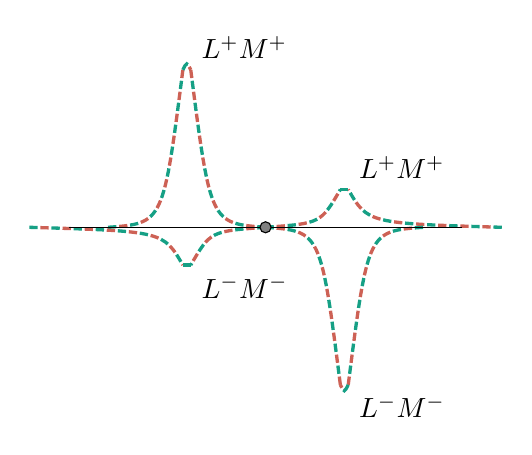
\begin{tikzpicture}
            % ON Center
            \draw[pomegranate!80, dash pattern= on 3pt off 5pt, dash phase=4pt, very thick] (-2.00, 0.00) .. controls (-1.30, 0.05) .. (-1.05, 2.00);
            \draw[pomegranate!80, dash pattern= on 3pt off 5pt, dash phase=4pt, very thick] (-1.05, 2.00) .. controls (-1.00, 2.10) .. (-0.95, 2.00);
            \draw[pomegranate!80, dash pattern= on 3pt off 5pt, dash phase=4pt, very thick] ( 0.00, 0.00) .. controls (-0.70, 0.05) .. (-0.95, 2.00);
            \draw[greensea,       dash pattern= on 3pt off 5pt, very thick]                 (-2.00, 0.00) .. controls (-1.30, 0.05) .. (-1.05, 2.00);
            \draw[greensea,       dash pattern= on 3pt off 5pt, very thick]                 (-1.05, 2.00) .. controls (-1.00, 2.10) .. (-0.95, 2.00);
            \draw[greensea,       dash pattern= on 3pt off 5pt, very thick]                 ( 0.00, 0.00) .. controls (-0.70, 0.05) .. (-0.95, 2.00)
                 node[color=black, anchor=south west] {$L^+M^+$};
            % OFF Surround
            \draw[pomegranate!80, dash pattern= on 3pt off 5pt, dash phase=4pt, very thick] (-3.00, 0.00) .. controls (-1.30,-0.05) .. (-1.05,-0.48);
            \draw[pomegranate!80, dash pattern= on 3pt off 5pt, dash phase=4pt, very thick] (-1.05,-0.48) .. controls (-1.00,-0.49) .. (-0.95,-0.48);
            \draw[pomegranate!80, dash pattern= on 3pt off 5pt, dash phase=4pt, very thick] ( 0.00, 0.00) .. controls (-0.70,-0.05) .. (-0.95,-0.48);
            \draw[greensea,       dash pattern= on 3pt off 5pt, very thick]                 (-3.00, 0.00) .. controls (-1.30,-0.05) .. (-1.05,-0.48);
            \draw[greensea,       dash pattern= on 3pt off 5pt, very thick]                 (-1.05,-0.48) .. controls (-1.00,-0.49) .. (-0.95,-0.48);
            \draw[greensea,       dash pattern= on 3pt off 5pt, very thick]                 ( 0.00, 0.00) .. controls (-0.70,-0.05) .. (-0.95,-0.48)
                 node[color=black, anchor=north west] {$L^-M^-$};
            % ON Center
            \draw[pomegranate!80, dash pattern= on 3pt off 5pt, dash phase=4pt, very thick] ( 0.00, 0.00) .. controls ( 0.70, 0.05) .. ( 0.95, 0.48);
            \draw[pomegranate!80, dash pattern= on 3pt off 5pt, dash phase=4pt, very thick] ( 1.05, 0.48) .. controls ( 1.00, 0.49) .. ( 0.95, 0.48);
            \draw[pomegranate!80, dash pattern= on 3pt off 5pt, dash phase=4pt, very thick] ( 3.00, 0.00) .. controls ( 1.30, 0.05) .. ( 1.05, 0.48);
            \draw[greensea,       dash pattern= on 3pt off 5pt, very thick]                 ( 0.00, 0.00) .. controls ( 0.70, 0.05) .. ( 0.95, 0.48);
            \draw[greensea,       dash pattern= on 3pt off 5pt, very thick]                 ( 1.05, 0.48) .. controls ( 1.00, 0.49) .. ( 0.95, 0.48);
            \draw[greensea,       dash pattern= on 3pt off 5pt, very thick]                 ( 3.00, 0.00) .. controls ( 1.30, 0.05) .. ( 1.05, 0.48)
                 node[color=black, anchor=south west] {$L^+M^+$};
            % OFF Surround
            \draw[pomegranate!80, dash pattern= on 3pt off 5pt, dash phase=4pt, very thick] ( 0.00, 0.00) .. controls ( 0.70,-0.05) .. ( 0.95,-2.00);
            \draw[pomegranate!80, dash pattern= on 3pt off 5pt, dash phase=4pt, very thick] ( 1.05,-2.00) .. controls ( 1.00,-2.10) .. ( 0.95,-2.00);
            \draw[pomegranate!80, dash pattern= on 3pt off 5pt, dash phase=4pt, very thick] ( 2.00, 0.00) .. controls ( 1.30,-0.05) .. ( 1.05,-2.00);
            \draw[greensea,       dash pattern= on 3pt off 5pt, very thick]                 ( 0.00, 0.00) .. controls ( 0.70,-0.05) .. ( 0.95,-2.00);
            \draw[greensea,       dash pattern= on 3pt off 5pt, very thick]                 ( 1.05,-2.00) .. controls ( 1.00,-2.10) .. ( 0.95,-2.00);
            \draw[greensea,       dash pattern= on 3pt off 5pt, very thick]                 ( 2.00, 0.00) .. controls ( 1.30,-0.05) .. ( 1.05,-2.00)
                 node[color=black, anchor=north west] {$L^-M^-$};
            % Reference line & point
            \draw                                                             (-2.50, 0.00) -- ( 2.50, 0.00);
            \filldraw[color=black, fill=gray]                                 ( 0.00, 0.00) circle (2pt);
            % Frame to ensure alignment:
            \draw[opacity=0]                                                  (-3.00, 2.50) rectangle (3.00, -2.50);
        \end{tikzpicture}
    }
    \caption{Light DO \\ Receptive Field} \label{fig:do-rf-inputs-light}
    \end{subfigure}%
    \begin{subfigure}{0.3\textwidth}
        \centering
        \resizebox{\textwidth}{!}{%
        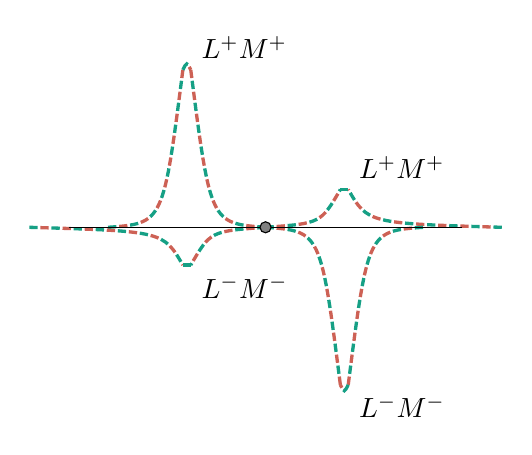
\begin{tikzpicture}
            % ON Center
            \draw[pomegranate!80, dash pattern= on 3pt off 5pt, dash phase=4pt, very thick] (-2.00, 0.00) .. controls (-1.30, 0.05) .. (-1.05, 2.00);
            \draw[pomegranate!80, dash pattern= on 3pt off 5pt, dash phase=4pt, very thick] (-1.05, 2.00) .. controls (-1.00, 2.10) .. (-0.95, 2.00);
            \draw[pomegranate!80, dash pattern= on 3pt off 5pt, dash phase=4pt, very thick] ( 0.00, 0.00) .. controls (-0.70, 0.05) .. (-0.95, 2.00);
            \draw[greensea,       dash pattern= on 3pt off 5pt, very thick]                 (-2.00, 0.00) .. controls (-1.30, 0.05) .. (-1.05, 2.00);
            \draw[greensea,       dash pattern= on 3pt off 5pt, very thick]                 (-1.05, 2.00) .. controls (-1.00, 2.10) .. (-0.95, 2.00);
            \draw[greensea,       dash pattern= on 3pt off 5pt, very thick]                 ( 0.00, 0.00) .. controls (-0.70, 0.05) .. (-0.95, 2.00)
                 node[color=black, anchor=south west] {$L^+M^+$};
            % OFF Surround
            \draw[pomegranate!80, dash pattern= on 3pt off 5pt, dash phase=4pt, very thick] (-3.00, 0.00) .. controls (-1.30,-0.05) .. (-1.05,-0.48);
            \draw[pomegranate!80, dash pattern= on 3pt off 5pt, dash phase=4pt, very thick] (-1.05,-0.48) .. controls (-1.00,-0.49) .. (-0.95,-0.48);
            \draw[pomegranate!80, dash pattern= on 3pt off 5pt, dash phase=4pt, very thick] ( 0.00, 0.00) .. controls (-0.70,-0.05) .. (-0.95,-0.48);
            \draw[greensea,       dash pattern= on 3pt off 5pt, very thick]                 (-3.00, 0.00) .. controls (-1.30,-0.05) .. (-1.05,-0.48);
            \draw[greensea,       dash pattern= on 3pt off 5pt, very thick]                 (-1.05,-0.48) .. controls (-1.00,-0.49) .. (-0.95,-0.48);
            \draw[greensea,       dash pattern= on 3pt off 5pt, very thick]                 ( 0.00, 0.00) .. controls (-0.70,-0.05) .. (-0.95,-0.48)
                 node[color=black, anchor=north west] {$L^-M^-$};
            % ON Center
            \draw[pomegranate!80, dash pattern= on 3pt off 5pt, dash phase=4pt, very thick] ( 0.00, 0.00) .. controls ( 0.70, 0.05) .. ( 0.95, 0.48);
            \draw[pomegranate!80, dash pattern= on 3pt off 5pt, dash phase=4pt, very thick] ( 1.05, 0.48) .. controls ( 1.00, 0.49) .. ( 0.95, 0.48);
            \draw[pomegranate!80, dash pattern= on 3pt off 5pt, dash phase=4pt, very thick] ( 3.00, 0.00) .. controls ( 1.30, 0.05) .. ( 1.05, 0.48);
            \draw[greensea,       dash pattern= on 3pt off 5pt, very thick]                 ( 0.00, 0.00) .. controls ( 0.70, 0.05) .. ( 0.95, 0.48);
            \draw[greensea,       dash pattern= on 3pt off 5pt, very thick]                 ( 1.05, 0.48) .. controls ( 1.00, 0.49) .. ( 0.95, 0.48);
            \draw[greensea,       dash pattern= on 3pt off 5pt, very thick]                 ( 3.00, 0.00) .. controls ( 1.30, 0.05) .. ( 1.05, 0.48)
                 node[color=black, anchor=south west] {$L^+M^+$};
            % OFF Surround
            \draw[pomegranate!80, dash pattern= on 3pt off 5pt, dash phase=4pt, very thick] ( 0.00, 0.00) .. controls ( 0.70,-0.05) .. ( 0.95,-2.00);
            \draw[pomegranate!80, dash pattern= on 3pt off 5pt, dash phase=4pt, very thick] ( 1.05,-2.00) .. controls ( 1.00,-2.10) .. ( 0.95,-2.00);
            \draw[pomegranate!80, dash pattern= on 3pt off 5pt, dash phase=4pt, very thick] ( 2.00, 0.00) .. controls ( 1.30,-0.05) .. ( 1.05,-2.00);
            \draw[greensea,       dash pattern= on 3pt off 5pt, very thick]                 ( 0.00, 0.00) .. controls ( 0.70,-0.05) .. ( 0.95,-2.00);
            \draw[greensea,       dash pattern= on 3pt off 5pt, very thick]                 ( 1.05,-2.00) .. controls ( 1.00,-2.10) .. ( 0.95,-2.00);
            \draw[greensea,       dash pattern= on 3pt off 5pt, very thick]                 ( 2.00, 0.00) .. controls ( 1.30,-0.05) .. ( 1.05,-2.00)
                 node[color=black, anchor=north west] {$L^-M^-$};
            % Reference line & point
            \draw                                                             (-2.50, 0.00) -- ( 2.50, 0.00);
            \filldraw[color=black, fill=gray]                                 ( 0.00, 0.00) circle (2pt);
            % Frame to ensure alignment:
            \draw[opacity=0]                                                  (-3.00, 2.50) rectangle (3.00, -2.50);
        \end{tikzpicture}
    }
    \caption{Dark DO \\ Receptive Field} \label{fig:do-rf-inputs-dark}
    \end{subfigure}%
    \par \bigskip
    \begin{subfigure}{0.3\textwidth}
        \centering
        \resizebox{\textwidth}{!}{%
        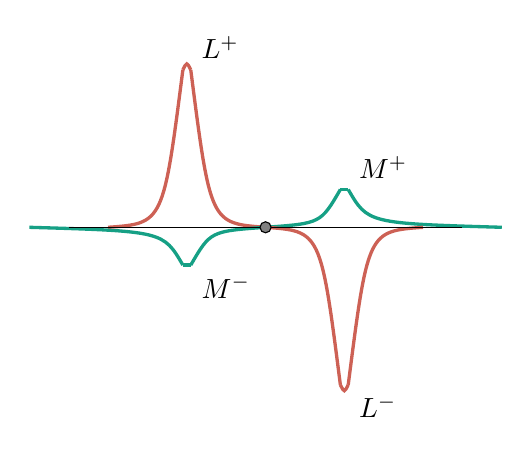
\begin{tikzpicture}
            % ON Center
            \draw[pomegranate!80, very thick] (-2.00, 0.00) .. controls (-1.30, 0.05) .. (-1.05, 2.00);
            \draw[pomegranate!80, very thick] (-1.05, 2.00) .. controls (-1.00, 2.10) .. (-0.95, 2.00);
            \draw[pomegranate!80, very thick] ( 0.00, 0.00) .. controls (-0.70, 0.05) .. (-0.95, 2.00)
                 node[color=black, anchor=south west] {$L^+$};
            % OFF Surround
            \draw[greensea,       very thick] (-3.00, 0.00) .. controls (-1.30,-0.05) .. (-1.05,-0.48);
            \draw[greensea,       very thick] (-1.05,-0.48) .. controls (-1.00,-0.49) .. (-0.95,-0.48);
            \draw[greensea,       very thick] ( 0.00, 0.00) .. controls (-0.70,-0.05) .. (-0.95,-0.48)
                 node[color=black, anchor=north west] {$M^-$};
            % ON Center
            \draw[greensea,       very thick] ( 0.00, 0.00) .. controls ( 0.70, 0.05) .. ( 0.95, 0.48);
            \draw[greensea,       very thick] ( 1.05, 0.48) .. controls ( 1.00, 0.49) .. ( 0.95, 0.48);
            \draw[greensea,       very thick] ( 3.00, 0.00) .. controls ( 1.30, 0.05) .. ( 1.05, 0.48)
                 node[color=black, anchor=south west] {$M^+$};
            % OFF Surround
            \draw[pomegranate!80, very thick] ( 0.00, 0.00) .. controls ( 0.70,-0.05) .. ( 0.95,-2.00);
            \draw[pomegranate!80, very thick] ( 1.05,-2.00) .. controls ( 1.00,-2.10) .. ( 0.95,-2.00);
            \draw[pomegranate!80, very thick] ( 2.00, 0.00) .. controls ( 1.30,-0.05) .. ( 1.05,-2.00)
                 node[color=black, anchor=north west] {$L^-$};
            % Reference line & point
            \draw                                                             (-2.50, 0.00) -- ( 2.50, 0.00);
            \filldraw[color=black, fill=gray]                                 ( 0.00, 0.00) circle (2pt);
            % Frame to ensure alignment:
            \draw[opacity=0]                                                  (-3.00, 2.50) rectangle (3.00, -2.50);
        \end{tikzpicture}
    }
    \caption{Red DO \\ Receptive Field} \label{fig:do-rf-inputs-red}
    \end{subfigure}%
    \begin{subfigure}{0.3\textwidth}
        \centering
        \resizebox{\textwidth}{!}{%
        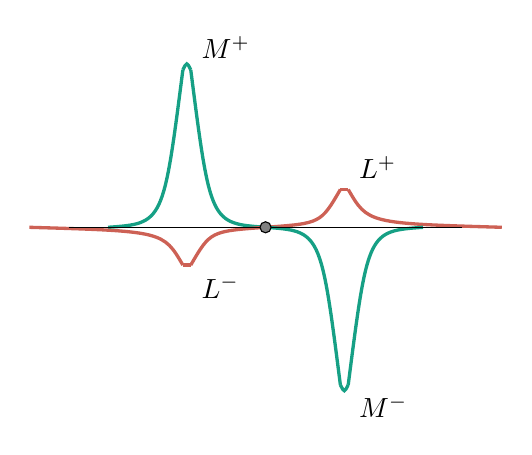
\begin{tikzpicture}
            % ON Center
            \draw[greensea, very thick] (-2.00, 0.00) .. controls (-1.30, 0.05) .. (-1.05, 2.00);
            \draw[greensea, very thick] (-1.05, 2.00) .. controls (-1.00, 2.10) .. (-0.95, 2.00);
            \draw[greensea, very thick] ( 0.00, 0.00) .. controls (-0.70, 0.05) .. (-0.95, 2.00)
                 node[color=black, anchor=south west] {$M^+$};
            % OFF Surround
            \draw[pomegranate!80,       very thick] (-3.00, 0.00) .. controls (-1.30,-0.05) .. (-1.05,-0.48);
            \draw[pomegranate!80,       very thick] (-1.05,-0.48) .. controls (-1.00,-0.49) .. (-0.95,-0.48);
            \draw[pomegranate!80,       very thick] ( 0.00, 0.00) .. controls (-0.70,-0.05) .. (-0.95,-0.48)
                 node[color=black, anchor=north west] {$L^-$};
            % ON Center
            \draw[pomegranate!80,       very thick] ( 0.00, 0.00) .. controls ( 0.70, 0.05) .. ( 0.95, 0.48);
            \draw[pomegranate!80,       very thick] ( 1.05, 0.48) .. controls ( 1.00, 0.49) .. ( 0.95, 0.48);
            \draw[pomegranate!80,       very thick] ( 3.00, 0.00) .. controls ( 1.30, 0.05) .. ( 1.05, 0.48)
                 node[color=black, anchor=south west] {$L^+$};
            % OFF Surround
            \draw[greensea, very thick] ( 0.00, 0.00) .. controls ( 0.70,-0.05) .. ( 0.95,-2.00);
            \draw[greensea, very thick] ( 1.05,-2.00) .. controls ( 1.00,-2.10) .. ( 0.95,-2.00);
            \draw[greensea, very thick] ( 2.00, 0.00) .. controls ( 1.30,-0.05) .. ( 1.05,-2.00)
                 node[color=black, anchor=north west] {$M^-$};
            % Reference line & point
            \draw                                                             (-2.50, 0.00) -- ( 2.50, 0.00);
            \filldraw[color=black, fill=gray]                                 ( 0.00, 0.00) circle (2pt);
            % Frame to ensure alignment:
            \draw[opacity=0]                                                  (-3.00, 2.50) rectangle (3.00, -2.50);
        \end{tikzpicture}
    }
    \caption{Green DO \\ Receptive Field} \label{fig:do-rf-inputs-green}
    \end{subfigure}%
    \par \bigskip
    \begin{subfigure}{0.3\textwidth}
        \centering
        \resizebox{\textwidth}{!}{%
        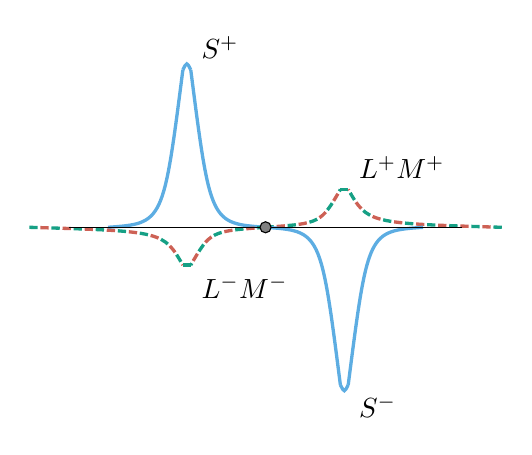
\begin{tikzpicture}
            % ON Center
            \draw[color=peter!80, very thick] (-2.00, 0.00) .. controls (-1.30, 0.05) .. (-1.05, 2.00);
            \draw[color=peter!80, very thick] (-1.05, 2.00) .. controls (-1.00, 2.10) .. (-0.95, 2.00);
            \draw[color=peter!80, very thick] ( 0.00, 0.00) .. controls (-0.70, 0.05) .. (-0.95, 2.00)
                 node[color=black, anchor=south west] {$S^+$};
            % OFF Surround
            \draw[pomegranate!80, dash pattern= on 3pt off 5pt, dash phase=4pt, very thick] (-3.00, 0.00) .. controls (-1.30,-0.05) .. (-1.05,-0.48);
            \draw[pomegranate!80, dash pattern= on 3pt off 5pt, dash phase=4pt, very thick] (-1.05,-0.48) .. controls (-1.00,-0.49) .. (-0.95,-0.48);
            \draw[pomegranate!80, dash pattern= on 3pt off 5pt, dash phase=4pt, very thick] ( 0.00, 0.00) .. controls (-0.70,-0.05) .. (-0.95,-0.48);
            \draw[greensea,       dash pattern= on 3pt off 5pt, very thick] (-3.00, 0.00) .. controls (-1.30,-0.05) .. (-1.05,-0.48);
            \draw[greensea,       dash pattern= on 3pt off 5pt, very thick] (-1.05,-0.48) .. controls (-1.00,-0.49) .. (-0.95,-0.48);
            \draw[greensea,       dash pattern= on 3pt off 5pt, very thick] ( 0.00, 0.00) .. controls (-0.70,-0.05) .. (-0.95,-0.48)
                 node[color=black, anchor=north west] {$L^-M^-$};
            % ON Center
            \draw[pomegranate!80, dash pattern= on 3pt off 5pt, dash phase=4pt, very thick] ( 0.00, 0.00) .. controls ( 0.70, 0.05) .. ( 0.95, 0.48);
            \draw[pomegranate!80, dash pattern= on 3pt off 5pt, dash phase=4pt, very thick] ( 1.05, 0.48) .. controls ( 1.00, 0.49) .. ( 0.95, 0.48);
            \draw[pomegranate!80, dash pattern= on 3pt off 5pt, dash phase=4pt, very thick] ( 3.00, 0.00) .. controls ( 1.30, 0.05) .. ( 1.05, 0.48);
            \draw[greensea,       dash pattern= on 3pt off 5pt, very thick] ( 0.00, 0.00) .. controls ( 0.70, 0.05) .. ( 0.95, 0.48);
            \draw[greensea,       dash pattern= on 3pt off 5pt, very thick] ( 1.05, 0.48) .. controls ( 1.00, 0.49) .. ( 0.95, 0.48);
            \draw[greensea,       dash pattern= on 3pt off 5pt, very thick] ( 3.00, 0.00) .. controls ( 1.30, 0.05) .. ( 1.05, 0.48)
                 node[color=black, anchor=south west] {$L^+M^+$};
            % OFF Surround
            \draw[color=peter!80, very thick] ( 0.00, 0.00) .. controls ( 0.70,-0.05) .. ( 0.95,-2.00);
            \draw[color=peter!80, very thick] ( 1.05,-2.00) .. controls ( 1.00,-2.10) .. ( 0.95,-2.00);
            \draw[color=peter!80, very thick] ( 2.00, 0.00) .. controls ( 1.30,-0.05) .. ( 1.05,-2.00)
                 node[color=black, anchor=north west] {$S^-$};
            % Reference line & point
            \draw                                                             (-2.50, 0.00) -- ( 2.50, 0.00);
            \filldraw[color=black, fill=gray]                                 ( 0.00, 0.00) circle (2pt);
            % Frame to ensure alignment:
            \draw[opacity=0]                                                  (-3.00, 2.50) rectangle (3.00, -2.50);
        \end{tikzpicture}
    }
    \caption{Blue DO \\ Receptive Field} \label{fig:do-rf-inputs-blue}
    \end{subfigure}%
    \begin{subfigure}{0.3\textwidth}
        \centering
        \resizebox{\textwidth}{!}{%
        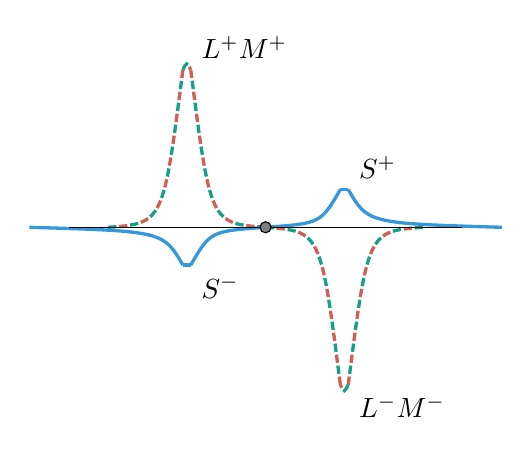
\begin{tikzpicture}
            % ON Center
            \draw[pomegranate!80, dash pattern= on 3pt off 5pt, dash phase=4pt, very thick] (-2.00, 0.00) .. controls (-1.30, 0.05) .. (-1.05, 2.00);
            \draw[pomegranate!80, dash pattern= on 3pt off 5pt, dash phase=4pt, very thick] (-1.05, 2.00) .. controls (-1.00, 2.10) .. (-0.95, 2.00);
            \draw[pomegranate!80, dash pattern= on 3pt off 5pt, dash phase=4pt, very thick] ( 0.00, 0.00) .. controls (-0.70, 0.05) .. (-0.95, 2.00);
            \draw[greensea,       dash pattern= on 3pt off 5pt, very thick]                 (-2.00, 0.00) .. controls (-1.30, 0.05) .. (-1.05, 2.00);
            \draw[greensea,       dash pattern= on 3pt off 5pt, very thick]                 (-1.05, 2.00) .. controls (-1.00, 2.10) .. (-0.95, 2.00);
            \draw[greensea,       dash pattern= on 3pt off 5pt, very thick]                 ( 0.00, 0.00) .. controls (-0.70, 0.05) .. (-0.95, 2.00)
                 node[color=black, anchor=south west] {$L^+M^+$};
            % OFF Surround
            \draw[color=peter,       very thick] (-3.00, 0.00) .. controls (-1.30,-0.05) .. (-1.05,-0.48);
            \draw[color=peter,       very thick] (-1.05,-0.48) .. controls (-1.00,-0.49) .. (-0.95,-0.48);
            \draw[color=peter,       very thick] ( 0.00, 0.00) .. controls (-0.70,-0.05) .. (-0.95,-0.48)
                 node[color=black, anchor=north west] {$S^-$};
            % ON Center
            \draw[color=peter,       very thick] ( 0.00, 0.00) .. controls ( 0.70, 0.05) .. ( 0.95, 0.48);
            \draw[color=peter,       very thick] ( 1.05, 0.48) .. controls ( 1.00, 0.49) .. ( 0.95, 0.48);
            \draw[color=peter,       very thick] ( 3.00, 0.00) .. controls ( 1.30, 0.05) .. ( 1.05, 0.48)
                 node[color=black, anchor=south west] {$S^+$};
            % OFF Surround
            \draw[pomegranate!80, dash pattern= on 3pt off 5pt, dash phase=4pt, very thick] ( 0.00, 0.00) .. controls ( 0.70,-0.05) .. ( 0.95,-2.00);
            \draw[pomegranate!80, dash pattern= on 3pt off 5pt, dash phase=4pt, very thick] ( 1.05,-2.00) .. controls ( 1.00,-2.10) .. ( 0.95,-2.00);
            \draw[pomegranate!80, dash pattern= on 3pt off 5pt, dash phase=4pt, very thick] ( 2.00, 0.00) .. controls ( 1.30,-0.05) .. ( 1.05,-2.00);
            \draw[greensea,       dash pattern= on 3pt off 5pt, very thick]                 ( 0.00, 0.00) .. controls ( 0.70,-0.05) .. ( 0.95,-2.00);
            \draw[greensea,       dash pattern= on 3pt off 5pt, very thick]                 ( 1.05,-2.00) .. controls ( 1.00,-2.10) .. ( 0.95,-2.00);
            \draw[greensea,       dash pattern= on 3pt off 5pt, very thick]                 ( 2.00, 0.00) .. controls ( 1.30,-0.05) .. ( 1.05,-2.00)
                 node[color=black, anchor=north west] {$L^-M^-$};
            % Reference line & point
            \draw                                                             (-2.50, 0.00) -- ( 2.50, 0.00);
            \filldraw[color=black, fill=gray]                                 ( 0.00, 0.00) circle (2pt);
            % Frame to ensure alignment:
            \draw[opacity=0]                                                  (-3.00, 2.50) rectangle (3.00, -2.50);
        \end{tikzpicture}
    }
    \caption{Yellow DO \\ Receptive Field} \label{fig:do-rf-inputs-yellow}
    \end{subfigure}%
    \caption{Double-opponent receptive fields utilized in \textit{Opponent Processing of Receptive Fields}.}
    \label{fig:do-rf-inputs}
\end{figure}
\clearpage
}

\subsection{Discrete Wavelet Transform in Opponent Colorspace}

Previous work by Penacchio \textit{et al.} \cite{otazu:plosive} utilized a discrete wavelet transform (DWT) to decompose a greyscale image into its oriented edge components, at scales. In the context of our current research, this could be thought of as representing achromatic double-opponent cells; the response is greatest at luminosity boundaries, and nonexistent on surfaces or at chromatic changes. In this work we extend their approach to the opponent colorspace and examine its applicability as a replacement of the previously detailed \textit{Opponent Processing of Neural Receptive Fields}.

Unlike the previously presented color descriptor, this transformation begins, not with the convolution step, but instead with a colorspace transformation. We convert the image from RGB to \textit{CIE} $L^*a^*b^*$. This colorspace separates luminance from it's two opponent color channels. The two color channels are $0$ centered; with positive and negative values in $a^*$ denoting redness and greenness, respectively, while positive and negative values in the $b^*$ channel indicate blueness and yellowness, respectively. The luminance channel, $L^*$, scales from $0$ to $100$, $0$ being total darkness, $100$ being pure brightness. We subtract $50$ from this channel to obtain a $0$ centered range of luminance. We consider positive values to define lightness and negative values darkness.

We then apply the DWT to this modified \textit{CIE} $L^*a^*b^*$ colorspace. Similar to the gaussian convolutions in the previous method, this transformation can be interpreted as representing processing in a cell's receptive field. That is, the activity of a particular cell is now defined, not just by its own activity, but also of the activity of the cells around it.

At each scale we further decompose the image into it's oriented signal components, our orientation and scale selective double-opponent cell activity. At each scale, we retain the residual 

The key difference here being that the DWT is applied \textit{in} the opponent colorspace, while in our previous approach the convolutions are applied to the raw L, M, and S input, in order to obtain the opponent colors.

Following multiresolution and orientation decomposition, all wavelet and residual planes are $0$ centered, thus we can easily split them into independent opponent components:
\begin{align}
    Light  &=   max(0, L^*-50)   \\
    Dark   &= | min(0, L^*-50) | \\
    Red    &=   max(0, a^*)      \\
    Green  &= | min(0, a^*) |    \\
    Blue   &=   max(0, b^*)      \\
    Yellow &= | min(0, b^*) |
\end{align}

The result of this process can be seen in the Appendix, Figure \ref{fig:transform-dwt}.

\bigskip
\textbf{//TODO} \textit{SUMMARY PARAGRAPH ON PROS/CONS}
\bigskip


\subsection*{Neurodynamical Processing}

Stage I of the proposed method focuses on the description of color in a biologically meaningful form, of which we've described two distinct approaches. Stage II is to further process this data in an iterative computational model of neurodynamical processes, as defined in Equations \ref{eq:delta-x} and \ref{eq:delta-y}. The input stimulus, from Stage I, at time $\tau$, $I^\tau_{i\gamma\sigma\theta}$ drives the model and mainly determines its response. The normalization of the stimulus at each time step is extended from that proposed by Li \cite{li:1999} and Penacchio \cite{penacchio:2013}. We normalize within each color channel ($\gamma$), scale ($\sigma$), and orientation ($\theta$). At the first time step, $I^1_{i\gamma\sigma\theta}$ is used to bootstrap the model and set as the initial excitation response, $x_{i\gamma\sigma\theta}$.

$x_{i\gamma\sigma\theta}$ can be viewed as a model of retinotopic excitation hypercolumns in V1, with $i$ specifying the retinally mapped location of the hypercolumn. Similarly, $y_{i\gamma\sigma\theta}$ may be interpreted as its retinotopic inhibitory counterpart. $\dot{x}_{i\gamma\sigma\theta}$ and $\dot{y}_{i\gamma\sigma\theta}$, then, are the change in excitatory and inhibitory membrane potentials over time, respectively, and follow the equations:
\begin{align}
    \dot{x}_{i\gamma\sigma\theta} &= \begin{aligned}[t]
        & - \alpha_{x}x_{i\gamma\sigma\theta} \label{eq:delta-x} \\
        & - g_y(y_{i\gamma\sigma\theta}) \\
        & - \sum\nolimits_{\gamma' \neq \text{opp($\gamma$)},\Delta_{\sigma},\Delta_{\theta} \neq 0}
            \Psi(\gamma',\Delta_{\sigma},\Delta_{\theta})
            g_y(y_{i\gamma\sigma + \Delta_{\sigma\theta} + \Delta_{\theta}})
            + J_0g_x(x_{i\gamma\sigma\theta}) \\
        & + \sum\nolimits_{j \neq i,\gamma' \neq \text{opp($\gamma$)},\sigma'\theta'}
            J_{[i\gamma\sigma\theta, j\gamma'\sigma'\theta']}g_x(x_{j\gamma'\sigma'\theta'})) \\
        & + I^\tau_{i\gamma\sigma\theta} \\
        & + I_0
        \end{aligned} \\
    \dot{y}_{i\gamma\sigma\theta} &= \begin{aligned}[t]
        & - \alpha_{y}Y_{i\gamma\sigma\theta} \label{eq:delta-y} \\
        & + g_x(X_{i\gamma\sigma\theta}) \\
        & + \sum\nolimits_{j \neq i, \gamma'\sigma'\theta'}
            W_{[i\gamma\sigma\theta, j\gamma'\sigma'\theta']}g_x(x_{j\gamma'\sigma'\theta'}) \\
        & + I_{c}
       \end{aligned}
\end{align}
where $\alpha_{x}x_{i\gamma\sigma\theta}$ and $\alpha_{y}Y_{i\gamma\sigma\theta}$ model the decay to the resting potential, $g_x(x)$ and $g_y(y)$ are sigmoid-like functions modeling cells' firing rates in response to membrane potentials $x$ and $y$, respectively, $\Psi(\gamma',\Delta_{\sigma},\Delta_{\theta}) \leq 1$ is the spread of inhibition within a hypercolumn, $J_0g_x(x_{i\gamma\sigma\theta})$ is self-excitation, and $I_c$ is background noise \cite{li:1999}.
Any cell can interact with another by exciting it or inhibiting it, via monosynaptic excitation through excitatory-excitatory horizontal connections, or disynaptic inhibition through excitatory-inhibitory connections, respectively \cite{penacchio:2013}. Such interactions are modeled between cells within and across hypercolumns; color, scale, and orientation, as well as between cells within and across cell classes; double-opponent and single-opponent. These cellular interactions are defined by $J_{[i\gamma\sigma\theta, j\gamma'\sigma'\theta']}$ (excitatory) and $W_{[i\gamma\sigma\theta, j\gamma'\sigma'\theta']}$ (inhibitory). 

\subsubsection*{Orientation ($\theta$)}
The excitatory and inhibitory interactions between orientation specific double-opponent cells are exactly as those defined by Penacchio \cite{penacchio:2013} and Li \cite{li:1999}. Single-opponent cells, introduced in our work, are non-directional; they have no preferred orientation $\theta$. $\Delta\theta$ is thus not computable and so this class of cells do not \textit{inhibit} the activity of other cells. Single-opponent cells do not contribute to $W$. In order to explore 'fill in' effects, however, we support parameterization of \textit{excitatory} weights to and from single-opponent and double-opponent cells. This weight functions as $\Delta\theta$ and is equal for all preferred orientations of the double-opponent cells. These interactions are modeled by a circular-symmetric gaussian in $J$.

\subsubsection*{Scale ($\sigma$)}
As in Penacchio \cite{penacchio:2013}, we decompose the input signal into signal at different scales. This reflect single-opponent and double-opponent cells' spatial frequency selectivity derived from their receptive fields. While this confers a level of scale invariance to the model, the primate visual cortex is not completely scale invariant and nor should our model be. Both image transformation methods presented in Stage I inherently represent activity at lower spatial frequencies with higher response.

\subsubsection*{Color ($\gamma$)}
We introduce a novel concept to the neurodynamical model framework developed by Li \cite{li:1999} and Penacchio \cite{penacchio:2013}: color. Unfortunately, the structural organization of color preferring cells and the connections between them is not well understood and leading theories are still quite controversial \cite{shapley:2011}. We herein define a set of \textit{logical} rules of interaction opponent color cells (including achromatic cells).

If a cell is stimulated, it excites nearby cells of the same orientation and scale preference, in any color channel other than its opponent. Conversely, a stimulated cell will inhibit nearby cells of the same orientation and scale preference, only in its opponent color channel. For example, stimulation of a DO cell preferring 'yellow' vertical edges will excite a DO cell preferring 'red' vertical edges at the same location. It will equally excite 'green', 'light', and 'dark' cells preferring the same orientation in the same location. It will not, however, excite cells of its opponent color 'blue'. In fact, it will inhibit activity in 'blue' cells preferring this same orientation in the same location.

We propose that these rules of interaction are logical as only opponent colors are mutually exclusive. While a bluish yellow line is not permissible in the opponent colorspace, a bluish green, bluish red, bright blue, or dark blue line is entirely plausible. Each of the possible combinations are equally probable and so the excitatory-excitatory connections between cells of these color preferences are equally weighed. These excitatory and inhibitory rules are encoded in $J$ and $W$, respectively.

\subsubsection*{Activity Normalization ($I_0$)}
The general and local normalization of activities \cite{heeger:1992} has been extended from its used by Li \cite{li:1999} and Penacchio \cite{penacchio:2013}. We normalize excitatory membrane potentials within double-opponent cells of similar location ($i$), color ($\gamma$), scale ($\sigma$), and orientation ($\theta$) preferences. Likewise we normalize single-opponent cells of similar location ($i$), color ($\gamma$), scale ($\sigma$). We found it important to normalize the activity of these two classes of neurons independently as the information encoded by each is radically different: localized edge information by double-opponent cells, and extensive surface information by single-opponent cells.

% FIGURE: Bowtie Excitatory Interaction Maps
\afterpage{%
\begin{figure}[htbp!] \label{fig:bowtie-excite-maps}
    \centering
    \begin{subfigure}[b]{0.2\textwidth}
            \centering
            \captionsetup{justification=centering}
            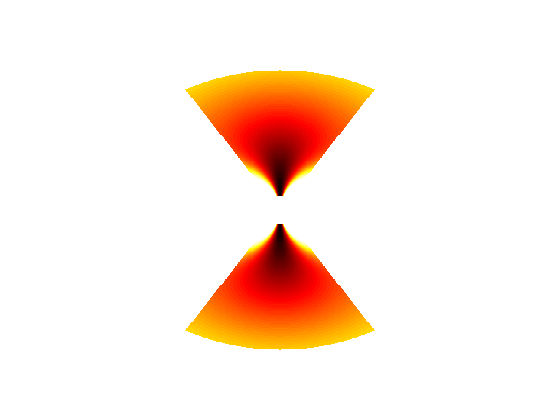
\includegraphics[width=.85\linewidth]{map-j_1_1}
            \caption{\\ Verical DO \\ \& Verical DO}
    \end{subfigure}%
    \begin{subfigure}[b]{0.2\textwidth}
            \centering
            \captionsetup{justification=centering}
            
\includegraphics[width=.85\linewidth]{map-j_1_2}
            \caption{\\ Verical DO \\ \& Diagonal DO}
    \end{subfigure}%
    \begin{subfigure}[b]{0.2\textwidth}
            \centering
            \captionsetup{justification=centering}
            
\includegraphics[width=.85\linewidth]{map-j_blank}
            \caption{\\ Verical DO \\ \& Horizontal DO}
    \end{subfigure}%
    \begin{subfigure}[b]{0.2\textwidth}
            \centering
            \captionsetup{justification=centering}
            
\includegraphics[width=.85\linewidth]{map-j_1_4}
            \caption{\\ Verical DO \\ \& Non-Oriented SO}
    \end{subfigure}%
    \par \bigskip
    \begin{subfigure}[b]{0.2\textwidth}
            \centering
            \captionsetup{justification=centering}
            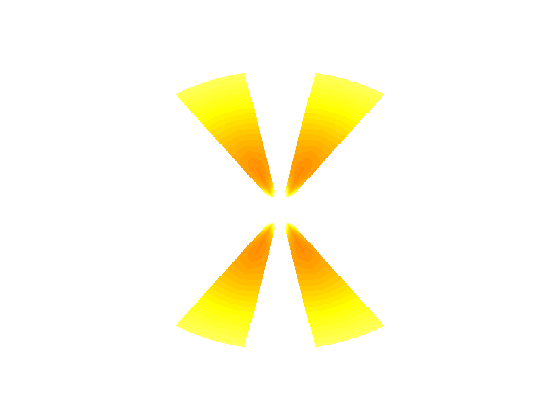
\includegraphics[width=.85\linewidth]{map-j_2_1}
            \caption{\\ Diagonal DO \\ \& Verical DO}
    \end{subfigure}%
    \begin{subfigure}[b]{0.2\textwidth}
            \centering
            \captionsetup{justification=centering}
            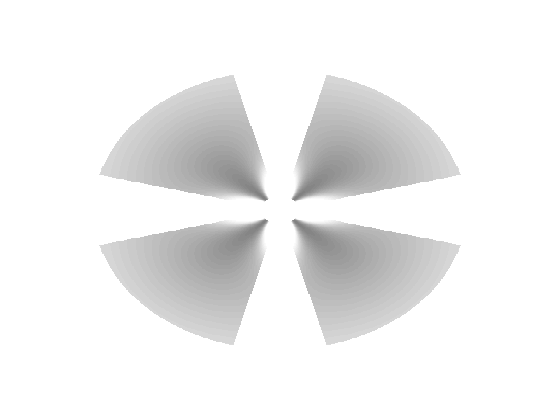
\includegraphics[width=.85\linewidth]{map-j_2_2}
            \caption{\\ Diagonal DO \\ \& Diagonal DO}
    \end{subfigure}%
    \begin{subfigure}[b]{0.2\textwidth}
            \centering
            \captionsetup{justification=centering}
            
\includegraphics[width=.85\linewidth]{map-j_2_3}
            \caption{\\ Diagonal DO \\ \& Horizontal DO}
    \end{subfigure}%
    \begin{subfigure}[b]{0.2\textwidth}
            \centering
            \captionsetup{justification=centering}
            
\includegraphics[width=.85\linewidth]{map-j_2_4}
            \caption{\\ Diagonal DO \\ \& Non-Oriented SO}
    \end{subfigure}%
    \par \bigskip
    \begin{subfigure}[b]{0.2\textwidth}
            \centering
            \captionsetup{justification=centering}
            
\includegraphics[width=.85\linewidth]{map-j_blank}
            \caption{\\ Horizontal DO \\ \& Verical DO}
    \end{subfigure}%
    \begin{subfigure}[b]{0.2\textwidth}
            \centering
            \captionsetup{justification=centering}
            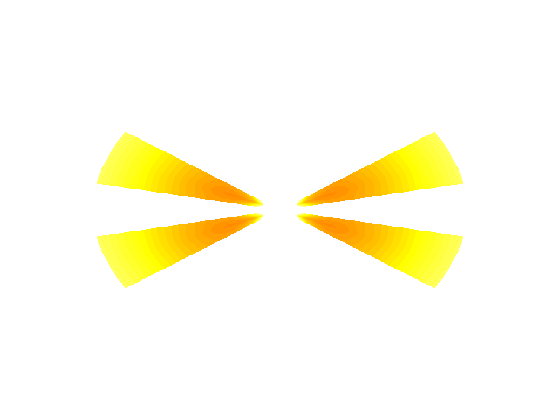
\includegraphics[width=.85\linewidth]{map-j_3_2}
            \caption{\\ Horizontal DO \\ \& Diagonal DO}
    \end{subfigure}%
    \begin{subfigure}[b]{0.2\textwidth}
            \centering
            \captionsetup{justification=centering}
            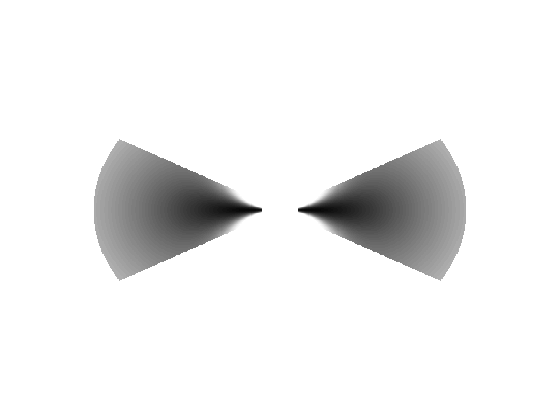
\includegraphics[width=.85\linewidth]{map-j_3_3}
            \caption{\\ Horizontal DO \\ \& Horizontal DO}
    \end{subfigure}
    \begin{subfigure}[b]{0.2\textwidth}
            \centering
            \captionsetup{justification=centering}
            
\includegraphics[width=.85\linewidth]{map-j_3_4}
            \caption{\\ Horizontal DO \\ \& Non-Oriented SO}
    \end{subfigure}%
    \par \bigskip
    \begin{subfigure}[b]{0.2\textwidth}
            \centering
            \captionsetup{justification=centering}
            
\includegraphics[width=.85\linewidth]{map-j_4_1}
            \caption{\\ Non-Oriented SO \\ \& Verical DO}
    \end{subfigure}%
    \begin{subfigure}[b]{0.2\textwidth}
            \centering
            \captionsetup{justification=centering}
            
\includegraphics[width=.85\linewidth]{map-j_4_2}
            \caption{\\ Non-Oriented SO \\ \& Diagonal DO}
    \end{subfigure}%
    \begin{subfigure}[b]{0.2\textwidth}
            \centering
            \captionsetup{justification=centering}
            
\includegraphics[width=.85\linewidth]{map-j_4_3}
            \caption{\\ Non-Oriented SO \\ \& Horizontal DO}
    \end{subfigure}
    \begin{subfigure}[b]{0.2\textwidth}
            \centering
            \captionsetup{justification=centering}
            
\includegraphics[width=.85\linewidth]{map-j_4_4}
            \caption{\\ Non-Oriented SO \\ \& Non-Oriented SO}
    \end{subfigure}%
    \caption{Graphical representation of \textit{excitatory} interaction weights ($J$) between vertical, diagonal, and horizontal double-opponent cells and single-opponent cells.}
\end{figure}
\clearpage
}
% FIGURE: Bowtie Inhibitory Interaction Maps
\afterpage{%
\begin{figure}[htbp!] \label{fig:bowtie-excite-maps}
    \centering
    \begin{subfigure}[b]{0.2\textwidth}
            \centering
            \captionsetup{justification=centering}
            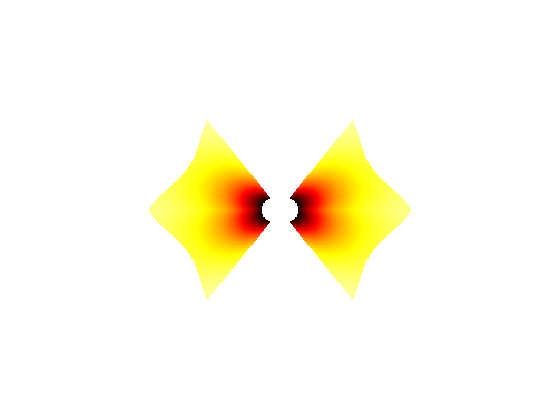
\includegraphics[width=.85\linewidth]{map-w_1_1}
            \caption{\\ Verical DO \\ \& Verical DO}
    \end{subfigure}%
    \begin{subfigure}[b]{0.2\textwidth}
            \centering
            \captionsetup{justification=centering}
            
\includegraphics[width=.85\linewidth]{map-w_1_2}
            \caption{\\ Verical DO \\ \& Diagonal DO}
    \end{subfigure}%
    \begin{subfigure}[b]{0.2\textwidth}
            \centering
            \captionsetup{justification=centering}
            
\includegraphics[width=.85\linewidth]{map-w_blank}
            \caption{\\ Verical DO \\ \& Horizontal DO}
    \end{subfigure}%
    \begin{subfigure}[b]{0.2\textwidth}
            \centering
            \captionsetup{justification=centering}
            
\includegraphics[width=.85\linewidth]{map-w_blank}
            \caption{\\ Verical DO \\ \& Non-Oriented SO}
    \end{subfigure}%
    \par \bigskip
    \begin{subfigure}[b]{0.2\textwidth}
            \centering
            \captionsetup{justification=centering}
            
\includegraphics[width=.85\linewidth]{map-w_2_1}
            \caption{\\ Diagonal DO \\ \& Verical DO}
    \end{subfigure}%
    \begin{subfigure}[b]{0.2\textwidth}
            \centering
            \captionsetup{justification=centering}
            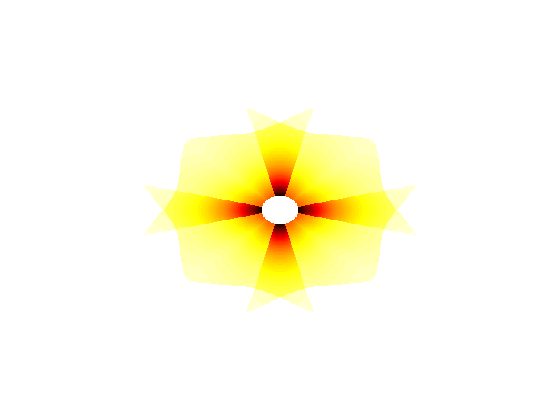
\includegraphics[width=.85\linewidth]{map-w_2_2}
            \caption{\\ Diagonal DO \\ \& Diagonal DO}
    \end{subfigure}%
    \begin{subfigure}[b]{0.2\textwidth}
            \centering
            \captionsetup{justification=centering}
            
\includegraphics[width=.85\linewidth]{map-w_2_3}
            \caption{\\ Diagonal DO \\ \& Horizontal DO}
    \end{subfigure}%
    \begin{subfigure}[b]{0.2\textwidth}
            \centering
            \captionsetup{justification=centering}
            
\includegraphics[width=.85\linewidth]{map-w_blank}
            \caption{\\ Diagonal DO \\ \& Non-Oriented SO}
    \end{subfigure}%
    \par \bigskip
    \begin{subfigure}[b]{0.2\textwidth}
            \centering
            \captionsetup{justification=centering}
            
\includegraphics[width=.85\linewidth]{map-w_blank}
            \caption{\\ Horizontal DO \\ \& Verical DO}
    \end{subfigure}%
    \begin{subfigure}[b]{0.2\textwidth}
            \centering
            \captionsetup{justification=centering}
            
\includegraphics[width=.85\linewidth]{map-w_3_2}
            \caption{\\ Horizontal DO \\ \& Diagonal DO}
    \end{subfigure}%
    \begin{subfigure}[b]{0.2\textwidth}
            \centering
            \captionsetup{justification=centering}
            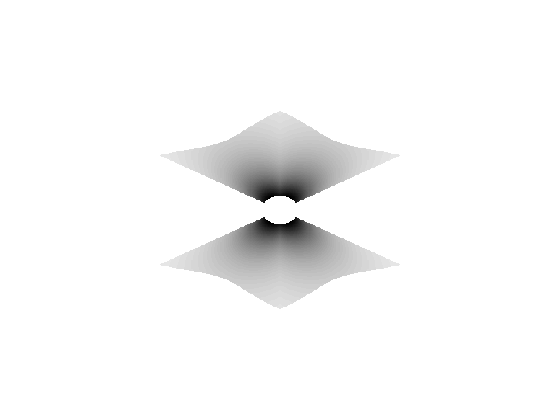
\includegraphics[width=.85\linewidth]{map-w_3_3}
            \caption{\\ Horizontal DO \\ \& Horizontal DO}
    \end{subfigure}%
    \begin{subfigure}[b]{0.2\textwidth}
            \centering
            \captionsetup{justification=centering}
            
\includegraphics[width=.85\linewidth]{map-w_blank}
            \caption{\\ Horizontal DO \\ \& Non-Oriented SO}
    \end{subfigure}%
    \par \bigskip
    \begin{subfigure}[b]{0.2\textwidth}
            \centering
            \captionsetup{justification=centering}
            
\includegraphics[width=.85\linewidth]{map-w_blank}
            \caption{\\ Non-Oriented SO \\ \& Verical DO}
    \end{subfigure}%
    \begin{subfigure}[b]{0.2\textwidth}
            \centering
            \captionsetup{justification=centering}
            
\includegraphics[width=.85\linewidth]{map-w_blank}
            \caption{\\ Non-Oriented SO \\ \& Diagonal DO}
    \end{subfigure}%
    \begin{subfigure}[b]{0.2\textwidth}
            \centering
            \captionsetup{justification=centering}
            
\includegraphics[width=.85\linewidth]{map-w_blank}
            \caption{\\ Non-Oriented SO \\ \& Horizontal DO}
    \end{subfigure}%
    \begin{subfigure}[b]{0.2\textwidth}
            \centering
            \captionsetup{justification=centering}
            
\includegraphics[width=.85\linewidth]{map-w_blank}
            \caption{\\ Non-Oriented SO \\ \& Non-Oriented SO}
    \end{subfigure}%
    \caption{Graphical representation of \textit{inhibitory} interaction weights ($W$) between vertical, diagonal, and horizontal double-opponent cells and single-opponent cells.}
\end{figure}
\clearpage
}

\newpage

%%%%%%%%%%%%%%%%%%%%%%%%%%%%%%%%%%%%%%%%%%%%%%%%%%%%%%%%%%%%%%%%
%
% EXPERIMENTS
%
% In which we describe the computational experiments employed,
% the psychophysical results expected, and the reasoning
% behind these expectations.
%
%%%%%%%%%%%%%%%%%%%%%%%%%%%%%%%%%%%%%%%%%%%%%%%%%%%%%%%%%%%%%%%%
\section{Experiments}

We evaluated the performance of our model by applying it to a number of test images seen to exhibit color induction effects. The expectation was that the model predict the perceived phenomena.

All experiments involved two or more test stimuli in which human observers can describe a difference between them. For example, most would describe the left inner ring in Figure \ref{fig:example} as being green and the right inner ring as being blue. As is shown, however, the two rings are physically identical; they have the exact same pixel values.

 All test images were paired such that the effects caused two physically similar regions to appear to be different colors. The output of the model was the retinotopic neural activity in each of the opponent channels. For each pair of test patches, we compared the activity to 1) identify differences in activity and 2) to observe differences in the \textit{direction} of activity. For example, in Figure \ref{img:test-circle-neon} we expect to see neural activity to the left inner circle move toward green on the red-green axis, and the right inner circle move toward blue on the blue-yellow axis. Because the unit of neuronal activity is arbitrary, it cannot be used to generate a color image of what the model predicts, a so called 'perceptual image'. However, the unit is self-consistent and so can be compared between stimuli to evaluate magnitude and direction of activity.

\textbf{//TODO} \textit{REWORK THIS PARAGRAPH.. IT'S NOT GREAT}

The perceived color is defined by the true color of the ring, the color(s) of the surrounding ring(s), and the interaction between them all.


%%%%%%%%%%%%%%%%%%%%%%%%%%%%%%%%%%%%%%%%%%%%%%%%%%%%%%%%%%%%%%%%
%
% RESULTS
%
% A presentation and review of the experiments to which the
% model was subjected.
%
%%%%%%%%%%%%%%%%%%%%%%%%%%%%%%%%%%%%%%%%%%%%%%%%%%%%%%%%%%%%%%%%
\section{Results}

\afterpage{%
\begin{figure}[H] \label{img:test-circle-a-opp-results}
    \centering
    \begin{subfigure}[b]{0.5\textwidth}
            \centering
            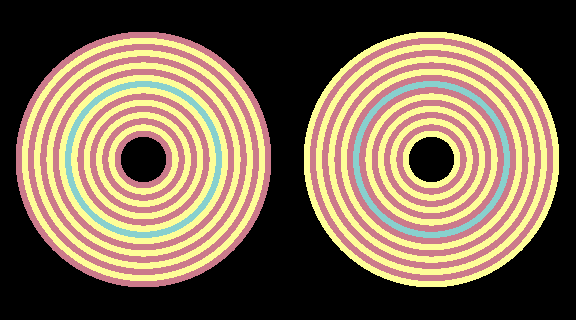
\includegraphics[width=230px]{test-circle-a}
            \caption{}
            \label{img:test-circle-a-opp}
    \end{subfigure}\\
    \begin{subfigure}[b]{0.25\textwidth}
            \centering
            
\includegraphics[width=100px, frame]{test-circle-a1-opp-ld}
            \caption{Light Dark}
            \label{img:test-circle-a1-opp-ld}
    \end{subfigure}%
    \begin{subfigure}[b]{0.25\textwidth}
            \centering
            
\includegraphics[width=100px, frame]{test-circle-a1-opp-ld-mask}
            \caption{Light Dark}
            \label{img:test-circle-a1-opp-ld-mask}
    \end{subfigure}%
    \begin{subfigure}[b]{0.25\textwidth}
            \centering
            
\includegraphics[width=100px, frame]{test-circle-a2-opp-ld-mask}
            \caption{Light Dark}
            \label{img:test-circle-a2-opp-ld-mask}
    \end{subfigure}%
    \begin{subfigure}[b]{0.25\textwidth}
            \centering
            
\includegraphics[width=100px, frame]{test-circle-a2-opp-ld}
            \caption{Light Dark}
            \label{img:test-circle-a2-opp-ld}
    \end{subfigure}\\
    \begin{subfigure}[b]{0.25\textwidth}
            \centering
            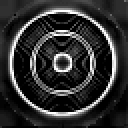
\includegraphics[width=100pt, frame]{test-circle-a1-opp-rg}
            \caption{Red Green}
            \label{img:test-circle-a1-opp-rg}
    \end{subfigure}%
    \begin{subfigure}[b]{0.25\textwidth}
            \centering
            
\includegraphics[width=100pt, frame]{test-circle-a1-opp-rg-mask}
            \caption{Red Green}
            \label{img:test-circle-a1-opp-rg-mask}
    \end{subfigure}%
    \begin{subfigure}[b]{0.25\textwidth}
            \centering
            
\includegraphics[width=100pt, frame]{test-circle-a2-opp-rg-mask}
            \caption{Red Green}
            \label{img:test-circle-a2-opp-rg-mask}
    \end{subfigure}%
    \begin{subfigure}[b]{0.25\textwidth}
            \centering
            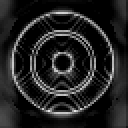
\includegraphics[width=100pt, frame]{test-circle-a2-opp-rg}
            \caption{Red Green}
            \label{img:test-circle-a2-opp-rg}
    \end{subfigure}\\
    \begin{subfigure}[b]{0.25\textwidth}
            \centering
            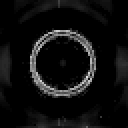
\includegraphics[width=100px, frame]{test-circle-a1-opp-by}
            \caption{Blue Yellow}
            \label{img:test-circle-a1-opp-by}
    \end{subfigure}%
    \begin{subfigure}[b]{0.25\textwidth}
            \centering
            
\includegraphics[width=100px, frame]{test-circle-a1-opp-by-mask}
            \caption{Blue Yellow}
            \label{img:test-circle-a1-opp-by-mask}
    \end{subfigure}%
    \begin{subfigure}[b]{0.25\textwidth}
            \centering
            
\includegraphics[width=100px, frame]{test-circle-a2-opp-by-mask}
            \caption{Blue Yellow}
            \label{img:test-circle-a2-opp-by-mask}
    \end{subfigure}%
    \begin{subfigure}[b]{0.25\textwidth}
            \centering
            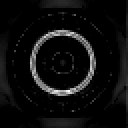
\includegraphics[width=100px, frame]{test-circle-a2-opp-by}
            \caption{Blue Yellow}
            \label{img:test-circle-a2-opp-by}
    \end{subfigure}
    \caption{Experimental results for the given test stimuli, \ref{img:test-circle-a-opp}, processed by the \textit{Opponent Processing of Receptive Fields} method. In \ref{img:test-circle-a1-opp-ld}, \ref{img:test-circle-a1-opp-rg}, and \ref{img:test-circle-a1-opp-by} we have the raw output of the L-D, R-G, and B-Y channels for the \textit{left} stimulus (which appears green). In \ref{img:test-circle-a2-opp-ld}, \ref{img:test-circle-a2-opp-rg}, and \ref{img:test-circle-a2-opp-by} we have the raw output of the L-D, R-G, and B-Y channels for the \textit{right} stimulus (which appears blue). In \ref{img:test-circle-a1-opp-ld-mask}, \ref{img:test-circle-a1-opp-rg-mask}, and \ref{img:test-circle-a1-opp-by-mask} we mask the raw output of the \textit{left} stimulus so as to isolate the test ring. In \ref{img:test-circle-a2-opp-ld-mask}, \ref{img:test-circle-a2-opp-rg-mask}, and \ref{img:test-circle-a2-opp-by-mask} we mask the raw output of the \textit{left} stimulus so as to isolate the test ring.}
\end{figure}
\clearpage
}

\afterpage{%
\begin{figure}[H] \label{img:test-circle-a-dwt-results}
    \centering
    \begin{subfigure}[b]{0.5\textwidth}
            \centering
            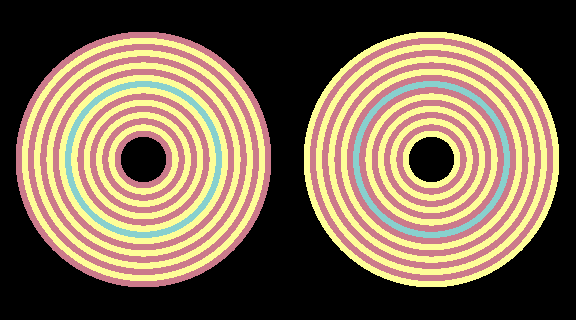
\includegraphics[width=230px]{test-circle-a}
            \caption{}
            \label{img:test-circle-a-dwt}
    \end{subfigure}\\
    \begin{subfigure}[b]{0.25\textwidth}
            \centering
            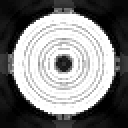
\includegraphics[width=100px, frame]{test-circle-a1-dwt-ld}
            \caption{Light Dark}
            \label{img:test-circle-a1-dwt-ld}
    \end{subfigure}%
    \begin{subfigure}[b]{0.25\textwidth}
            \centering
            
\includegraphics[width=100px, frame]{test-circle-a1-dwt-ld-mask}
            \caption{Light Dark}
            \label{img:test-circle-a1-dwt-ld-mask}
    \end{subfigure}%
    \begin{subfigure}[b]{0.25\textwidth}
            \centering
            
\includegraphics[width=100px, frame]{test-circle-a2-dwt-ld-mask}
            \caption{Light Dark}
            \label{img:test-circle-a2-dwt-ld-mask}
    \end{subfigure}%
    \begin{subfigure}[b]{0.25\textwidth}
            \centering
            \includegraphics[width=100px, frame]{test-circle-a2-dwt-ld}
            \caption{Light Dark}
            \label{img:test-circle-a2-dwt-ld}
    \end{subfigure}\\
    \begin{subfigure}[b]{0.25\textwidth}
            \centering
            \includegraphics[width=100pt, frame]{test-circle-a1-dwt-rg}
            \caption{Red Green}
            \label{img:test-circle-a1-dwt-rg}
    \end{subfigure}%
    \begin{subfigure}[b]{0.25\textwidth}
            \centering
            \includegraphics[width=100pt, frame]{test-circle-a1-dwt-rg-mask}
            \caption{Red Green}
            \label{img:test-circle-a1-dwt-rg-mask}
    \end{subfigure}%
    \begin{subfigure}[b]{0.25\textwidth}
            \centering
            \includegraphics[width=100pt, frame]{test-circle-a2-dwt-rg-mask}
            \caption{Red Green}
            \label{img:test-circle-a2-dwt-rg-mask}
    \end{subfigure}%
    \begin{subfigure}[b]{0.25\textwidth}
            \centering
            \includegraphics[width=100pt, frame]{test-circle-a2-dwt-rg}
            \caption{Red Green}
            \label{img:test-circle-a2-dwt-rg}
    \end{subfigure}\\
    \begin{subfigure}[b]{0.25\textwidth}
            \centering
            \includegraphics[width=100px, frame]{test-circle-a1-dwt-by}
            \caption{Blue Yellow}
            \label{img:test-circle-a1-dwt-by}
    \end{subfigure}%
    \begin{subfigure}[b]{0.25\textwidth}
            \centering
            \includegraphics[width=100px, frame]{test-circle-a1-dwt-by-mask}
            \caption{Blue Yellow}
            \label{img:test-circle-a1-dwt-by-mask}
    \end{subfigure}%
    \begin{subfigure}[b]{0.25\textwidth}
            \centering
            \includegraphics[width=100px, frame]{test-circle-a2-dwt-by-mask}
            \caption{Blue Yellow}
            \label{img:test-circle-a2-dwt-by-mask}
    \end{subfigure}%
    \begin{subfigure}[b]{0.25\textwidth}
            \centering
            \includegraphics[width=100px, frame]{test-circle-a2-dwt-by}
            \caption{Blue Yellow}
            \label{img:test-circle-a2-dwt-by}
    \end{subfigure}
    \caption{Experimental results for the given test stimuli, \ref{img:test-circle-a-dwt}, processed by the \textit{Discrete Wavelet Transform in Opponent Colorspace} method. In \ref{img:test-circle-a1-dwt-ld}, \ref{img:test-circle-a1-dwt-rg}, and \ref{img:test-circle-a1-dwt-by} we have the raw output of the L-D, R-G, and B-Y channels for the \textit{left} stimulus (which appears green). In \ref{img:test-circle-a2-dwt-ld}, \ref{img:test-circle-a2-dwt-rg}, and \ref{img:test-circle-a2-dwt-by} we have the raw output of the L-D, R-G, and B-Y channels for the \textit{right} stimulus (which appears blue). In \ref{img:test-circle-a1-dwt-ld-mask}, \ref{img:test-circle-a1-dwt-rg-mask}, and \ref{img:test-circle-a1-dwt-by-mask} we mask the raw output of the \textit{left} stimulus so as to isolate the test ring. In \ref{img:test-circle-a2-dwt-ld-mask}, \ref{img:test-circle-a2-dwt-rg-mask}, and \ref{img:test-circle-a2-dwt-by-mask} we mask the raw output of the \textit{left} stimulus so as to isolate the test ring.}
\end{figure}
\clearpage
}

\afterpage{%
\begin{figure}[H] \label{img:test-circle-neon-opp-results}
    \centering
    \begin{subfigure}[b]{0.5\textwidth}
            \centering
            \includegraphics[width=230px]{test-circle-neon}
            \caption{}
            \label{img:test-circle-neon-opp}
    \end{subfigure}\\
    \begin{subfigure}[b]{0.25\textwidth}
            \centering
            \includegraphics[width=100px, frame]{test-circle-neon-opp-a-ld}
            \caption{Light Dark}
            \label{img:test-circle-neon-opp-a-ld}
    \end{subfigure}%
    \begin{subfigure}[b]{0.25\textwidth}
            \centering
            \includegraphics[width=100px, frame]{test-circle-neon-opp-a-ld-mask}
            \caption{Light Dark}
            \label{img:test-circle-neon-opp-a-ld-mask}
    \end{subfigure}%
    \begin{subfigure}[b]{0.25\textwidth}
            \centering
            \includegraphics[width=100px, frame]{test-circle-neon-opp-b-ld-mask}
            \caption{Light Dark}
            \label{img:test-circle-neon-opp-b-ld-mask}
    \end{subfigure}%
    \begin{subfigure}[b]{0.25\textwidth}
            \centering
            \includegraphics[width=100px, frame]{test-circle-neon-opp-b-ld}
            \caption{Light Dark}
            \label{img:test-circle-neon-opp-b-ld}
    \end{subfigure}\\
    \begin{subfigure}[b]{0.25\textwidth}
            \centering
            \includegraphics[width=100pt, frame]{test-circle-neon-opp-a-rg}
            \caption{Red Green}
            \label{img:test-circle-neon-opp-a-rg}
    \end{subfigure}%
    \begin{subfigure}[b]{0.25\textwidth}
            \centering
            \includegraphics[width=100pt, frame]{test-circle-neon-opp-a-rg-mask}
            \caption{Red Green}
            \label{img:test-circle-neon-opp-a-rg-mask}
    \end{subfigure}%
    \begin{subfigure}[b]{0.25\textwidth}
            \centering
            \includegraphics[width=100pt, frame]{test-circle-neon-opp-b-rg-mask}
            \caption{Red Green}
            \label{img:test-circle-neon-opp-b-rg-mask}
    \end{subfigure}%
    \begin{subfigure}[b]{0.25\textwidth}
            \centering
            \includegraphics[width=100pt, frame]{test-circle-neon-opp-b-rg}
            \caption{Red Green}
            \label{img:test-circle-neon-opp-b-rg}
    \end{subfigure}\\
    \begin{subfigure}[b]{0.25\textwidth}
            \centering
            \includegraphics[width=100px, frame]{test-circle-neon-opp-a-by}
            \caption{Blue Yellow}
            \label{img:test-circle-neon-opp-a-by}
    \end{subfigure}%
    \begin{subfigure}[b]{0.25\textwidth}
            \centering
            \includegraphics[width=100px, frame]{test-circle-neon-opp-a-by-mask}
            \caption{Blue Yellow}
            \label{img:test-circle-neon-opp-a-by-mask}
    \end{subfigure}%
    \begin{subfigure}[b]{0.25\textwidth}
            \centering
            \includegraphics[width=100px, frame]{test-circle-neon-opp-b-by-mask}
            \caption{Blue Yellow}
            \label{img:test-circle-neon-opp-b-by-mask}
    \end{subfigure}%
    \begin{subfigure}[b]{0.25\textwidth}
            \centering
            \includegraphics[width=100px, frame]{test-circle-neon-opp-b-by}
            \caption{Blue Yellow}
            \label{img:test-circle-neon-opp-b-by}
    \end{subfigure}
    \caption{Experimental results for the given test stimuli, \ref{img:test-circle-neon-opp}, processed by the \textit{Opponent Processing of Receptive Fields} method. In \ref{img:test-circle-neon-opp-a-ld}, \ref{img:test-circle-neon-opp-a-rg}, and \ref{img:test-circle-neon-opp-a-by} we have the raw output of the L-D, R-G, and B-Y channels for the \textit{left} stimulus (which appears green). In \ref{img:test-circle-neon-opp-b-ld}, \ref{img:test-circle-neon-opp-b-rg}, and \ref{img:test-circle-neon-opp-b-by} we have the raw output of the L-D, R-G, and B-Y channels for the \textit{right} stimulus (which appears blue). In \ref{img:test-circle-neon-opp-a-ld-mask}, \ref{img:test-circle-neon-opp-a-rg-mask}, and \ref{img:test-circle-neon-opp-a-by-mask} we mask the raw output of the \textit{left} stimulus so as to isolate the test ring. In \ref{img:test-circle-neon-opp-b-ld-mask}, \ref{img:test-circle-neon-opp-b-rg-mask}, and \ref{img:test-circle-neon-opp-b-by-mask} we mask the raw output of the \textit{left} stimulus so as to isolate the test ring.}
\end{figure}
\clearpage
}

\afterpage{%
\begin{figure}[H] \label{img:test-circle-neon-dwt-results}
    \centering
    \begin{subfigure}[b]{0.5\textwidth}
            \centering
            \includegraphics[width=230px]{test-circle-neon}
            \caption{}
            \label{img:test-circle-neon-dwt}
    \end{subfigure}\\
    \begin{subfigure}[b]{0.25\textwidth}
            \centering
            \includegraphics[width=100px, frame]{test-circle-neon-dwt-a-ld}
            \caption{Light Dark}
            \label{img:test-circle-neon-dwt-a-ld}
    \end{subfigure}%
    \begin{subfigure}[b]{0.25\textwidth}
            \centering
            \includegraphics[width=100px, frame]{test-circle-neon-dwt-a-ld-mask}
            \caption{Light Dark}
            \label{img:test-circle-neon-dwt-a-ld-mask}
    \end{subfigure}%
    \begin{subfigure}[b]{0.25\textwidth}
            \centering
            \includegraphics[width=100px, frame]{test-circle-neon-dwt-b-ld-mask}
            \caption{Light Dark}
            \label{img:test-circle-neon-dwt-b-ld-mask}
    \end{subfigure}%
    \begin{subfigure}[b]{0.25\textwidth}
            \centering
            \includegraphics[width=100px, frame]{test-circle-neon-dwt-b-ld}
            \caption{Light Dark}
            \label{img:test-circle-neon-dwt-b-ld}
    \end{subfigure}\\
    \begin{subfigure}[b]{0.25\textwidth}
            \centering
            \includegraphics[width=100pt, frame]{test-circle-neon-dwt-a-rg}
            \caption{Red Green}
            \label{img:test-circle-neon-dwt-a-rg}
    \end{subfigure}%
    \begin{subfigure}[b]{0.25\textwidth}
            \centering
            \includegraphics[width=100pt, frame]{test-circle-neon-dwt-a-rg-mask}
            \caption{Red Green}
            \label{img:test-circle-neon-dwt-a-rg-mask}
    \end{subfigure}%
    \begin{subfigure}[b]{0.25\textwidth}
            \centering
            \includegraphics[width=100pt, frame]{test-circle-neon-dwt-b-rg-mask}
            \caption{Red Green}
            \label{img:test-circle-neon-dwt-b-rg-mask}
    \end{subfigure}%
    \begin{subfigure}[b]{0.25\textwidth}
            \centering
            \includegraphics[width=100pt, frame]{test-circle-neon-dwt-b-rg}
            \caption{Red Green}
            \label{img:test-circle-neon-dwt-b-rg}
    \end{subfigure}\\
    \begin{subfigure}[b]{0.25\textwidth}
            \centering
            \includegraphics[width=100px, frame]{test-circle-neon-dwt-a-by}
            \caption{Blue Yellow}
            \label{img:test-circle-neon-dwt-a-by}
    \end{subfigure}%
    \begin{subfigure}[b]{0.25\textwidth}
            \centering
            \includegraphics[width=100px, frame]{test-circle-neon-dwt-a-by-mask}
            \caption{Blue Yellow}
            \label{img:test-circle-neon-dwt-a-by-mask}
    \end{subfigure}%
    \begin{subfigure}[b]{0.25\textwidth}
            \centering
            \includegraphics[width=100px, frame]{test-circle-neon-dwt-b-by-mask}
            \caption{Blue Yellow}
            \label{img:test-circle-neon-dwt-b-by-mask}
    \end{subfigure}%
    \begin{subfigure}[b]{0.25\textwidth}
            \centering
            \includegraphics[width=100px, frame]{test-circle-neon-dwt-b-by}
            \caption{Blue Yellow}
            \label{img:test-circle-neon-dwt-b-by}
    \end{subfigure}
    \caption{Experimental results for the given test stimuli, \ref{img:test-circle-neon-dwt}, processed by the \textit{Discrete Wavelet Transform in Opponent Colorspace} method. In \ref{img:test-circle-neon-dwt-a-ld}, \ref{img:test-circle-neon-dwt-a-rg}, and \ref{img:test-circle-neon-dwt-a-by} we have the raw output of the L-D, R-G, and B-Y channels for the \textit{left} stimulus (which appears green). In \ref{img:test-circle-neon-dwt-b-ld}, \ref{img:test-circle-neon-dwt-b-rg}, and \ref{img:test-circle-neon-dwt-b-by} we have the raw output of the L-D, R-G, and B-Y channels for the \textit{right} stimulus (which appears blue). In \ref{img:test-circle-neon-dwt-a-ld-mask}, \ref{img:test-circle-neon-dwt-a-rg-mask}, and \ref{img:test-circle-neon-dwt-a-by-mask} we mask the raw output of the \textit{left} stimulus so as to isolate the test ring. In \ref{img:test-circle-neon-dwt-b-ld-mask}, \ref{img:test-circle-neon-dwt-b-rg-mask}, and \ref{img:test-circle-neon-dwt-b-by-mask} we mask the raw output of the \textit{left} stimulus so as to isolate the test ring.}
\end{figure}
\clearpage
}

\afterpage{%
\begin{figure}[H] \label{img:test-gradient-opp-results}
    \centering
    \begin{subfigure}[b]{1\textwidth}
            \centering
            \includegraphics[width=230px]{test-gradient}
            \caption{}
            \label{img:test-gradient-opp}
    \end{subfigure}\\
    \begin{subfigure}[b]{0.5\textwidth}
            \centering
            \includegraphics[width=108px, frame]{test-gradient-opp-ld}
            \caption{\\ Light-Dark Output}
            \label{img:test-gradient-opp-ld}
    \end{subfigure}%
    \begin{subfigure}[b]{0.5\textwidth}
            \centering
            \includegraphics[width=108px, frame]{test-gradient-opp-ld-mask}
            \caption{\\ Light-Dark Output (Enhanced)}
            \label{img:test-gradient-opp-ld-mask}
    \end{subfigure}\\
    \begin{subfigure}[b]{0.5\textwidth}
            \centering
            \includegraphics[width=108px, frame]{test-gradient-opp-rg}
            \caption{\\ Red-Green Output}
            \label{img:test-gradient-opp-rg}
    \end{subfigure}%
    \begin{subfigure}[b]{0.5\textwidth}
            \centering
            \includegraphics[width=108px, frame]{test-gradient-opp-rg-mask}
            \caption{\\ Red-Green Output (Enhanced)}
            \label{img:test-gradient-opp-rg-mask}
    \end{subfigure}\\
    \begin{subfigure}[b]{0.5\textwidth}
            \centering
            \includegraphics[width=108px, frame]{test-gradient-opp-by}
            \caption{\\ Blue-Yellow Output}
            \label{img:test-gradient-opp-by}
    \end{subfigure}%
    \begin{subfigure}[b]{0.5\textwidth}
            \centering
            \includegraphics[width=108px, frame]{test-gradient-opp-by-mask}
            \caption{\\ Blue-Yellow Output (Enhanced)}
            \label{img:test-gradient-opp-by-mask}
    \end{subfigure}
    \caption{Experimental results for the given test stimuli, \ref{img:test-gradient-opp}, processed by the \textit{Opponent Processing of Receptive Fields} method. In \ref{img:test-gradient-opp-ld}, \ref{img:test-gradient-opp-rg}, and \ref{img:test-gradient-opp-by} we have the raw output of the L-D, R-G, and B-Y channels. In \ref{img:test-gradient-opp-ld-mask}, \ref{img:test-gradient-opp-rg-mask}, and \ref{img:test-gradient-opp-by-mask} we mask the raw output so as to isolate and enhance the test patches.}
\end{figure}
\clearpage
}

\afterpage{%
\begin{figure}[H] \label{img:test-gradient-dwt-results}
    \centering
    \begin{subfigure}[b]{1\textwidth}
            \centering
            \includegraphics[width=230px]{test-gradient}
            \caption{}
            \label{img:test-gradient-dwt}
    \end{subfigure}\\
    \begin{subfigure}[b]{0.5\textwidth}
            \centering
            \includegraphics[width=108px, frame]{test-gradient-dwt-ld}
            \caption{\\ Light-Dark Output}
            \label{img:test-gradient-dwt-ld}
    \end{subfigure}%
    \begin{subfigure}[b]{0.5\textwidth}
            \centering
            \includegraphics[width=108px, frame]{test-gradient-dwt-ld-mask}
            \caption{\\ Light-Dark Output (Enhanced)}
            \label{img:test-gradient-dwt-ld-mask}
    \end{subfigure}\\
    \begin{subfigure}[b]{0.5\textwidth}
            \centering
            \includegraphics[width=108px, frame]{test-gradient-dwt-rg}
            \caption{\\ Red-Green Output}
            \label{img:test-gradient-dwt-rg}
    \end{subfigure}%
    \begin{subfigure}[b]{0.5\textwidth}
            \centering
            \includegraphics[width=108px, frame]{test-gradient-dwt-rg-mask}
            \caption{\\ Red-Green Output (Enhanced)}
            \label{img:test-gradient-dwt-rg-mask}
    \end{subfigure}\\
    \begin{subfigure}[b]{0.5\textwidth}
            \centering
            \includegraphics[width=108px, frame]{test-gradient-dwt-by}
            \caption{\\ Blue-Yellow Output}
            \label{img:test-gradient-dwt-by}
    \end{subfigure}%
    \begin{subfigure}[b]{0.5\textwidth}
            \centering
            \includegraphics[width=108px, frame]{test-gradient-dwt-by-mask}
            \caption{\\ Blue-Yellow Output (Enhanced)}
            \label{img:test-gradient-dwt-by-mask}
    \end{subfigure}
    \caption{Experimental results for the given test stimuli, \ref{img:test-gradient-dwt}, processed by the \textit{Discrete Wavelet Transform in Opponent Colorspace} method. In \ref{img:test-gradient-dwt-ld}, \ref{img:test-gradient-dwt-rg}, and \ref{img:test-gradient-dwt-by} we have the raw output of the L-D, R-G, and B-Y channels. In \ref{img:test-gradient-dwt-ld-mask}, \ref{img:test-gradient-dwt-rg-mask}, and \ref{img:test-gradient-dwt-by-mask} we mask the raw output so as to isolate and enhance the test patches.}
\end{figure}
\clearpage
}


\afterpage{%
\begin{figure}[H] \label{img:test-bars-opp-results}
    \centering
    \begin{subfigure}[b]{1\textwidth}
            \centering
            \includegraphics[width=230px]{test-bars}
            \caption{}
            \label{img:test-bars-opp}
    \end{subfigure}\\
    \begin{subfigure}[b]{0.5\textwidth}
            \centering
            \includegraphics[width=108px, frame]{test-bars-opp-ld}
            \caption{\\ Light-Dark Output}
            \label{img:test-bars-opp-ld}
    \end{subfigure}%
    \begin{subfigure}[b]{0.5\textwidth}
            \centering
            \includegraphics[width=108px, frame]{test-bars-opp-ld-mask}
            \caption{\\ Light-Dark Output (Enhanced)}
            \label{img:test-bars-opp-ld-mask}
    \end{subfigure}\\
    \begin{subfigure}[b]{0.5\textwidth}
            \centering
            \includegraphics[width=108px, frame]{test-bars-opp-rg}
            \caption{\\ Red-Green Output}
            \label{img:test-bars-opp-rg}
    \end{subfigure}%
    \begin{subfigure}[b]{0.5\textwidth}
            \centering
            \includegraphics[width=108px, frame]{test-bars-opp-rg-mask}
            \caption{\\ Red-Green Output (Enhanced)}
            \label{img:test-bars-opp-rg-mask}
    \end{subfigure}\\
    \begin{subfigure}[b]{0.5\textwidth}
            \centering
            \includegraphics[width=108px, frame]{test-bars-opp-by}
            \caption{\\ Blue-Yellow Output}
            \label{img:test-bars-opp-by}
    \end{subfigure}%
    \begin{subfigure}[b]{0.5\textwidth}
            \centering
            \includegraphics[width=108px, frame]{test-bars-opp-by-mask}
            \caption{\\ Blue-Yellow Output (Enhanced)}
            \label{img:test-bars-opp-by-mask}
    \end{subfigure}
    \caption{Experimental results for the given test stimuli, \ref{img:test-bars-opp}, processed by the \textit{Opponent Processing of Receptive Fields} method. In \ref{img:test-bars-opp-ld}, \ref{img:test-bars-opp-rg}, and \ref{img:test-bars-opp-by} we have the raw output of the L-D, R-G, and B-Y channels. In \ref{img:test-bars-opp-ld-mask}, \ref{img:test-bars-opp-rg-mask}, and \ref{img:test-bars-opp-by-mask} we mask the raw output so as to isolate and enhance the test patches.}
\end{figure}
\clearpage
}

\afterpage{%
\begin{figure}[H] \label{img:test-bars-dwt-results}
    \centering
    \begin{subfigure}[b]{1\textwidth}
            \centering
            \includegraphics[width=230px]{test-bars}
            \caption{}
            \label{img:test-bars-dwt}
    \end{subfigure}\\
    \begin{subfigure}[b]{0.5\textwidth}
            \centering
            \includegraphics[width=108px, frame]{test-bars-dwt-ld}
            \caption{\\ Light-Dark Output}
            \label{img:test-bars-dwt-ld}
    \end{subfigure}%
    \begin{subfigure}[b]{0.5\textwidth}
            \centering
            \includegraphics[width=108px, frame]{test-bars-dwt-ld-mask}
            \caption{\\ Light-Dark Output (Enhanced)}
            \label{img:test-bars-dwt-ld-mask}
    \end{subfigure}\\
    \begin{subfigure}[b]{0.5\textwidth}
            \centering
            \includegraphics[width=108px, frame]{test-bars-dwt-rg}
            \caption{\\ Red-Green Output}
            \label{img:test-bars-dwt-rg}
    \end{subfigure}%
    \begin{subfigure}[b]{0.5\textwidth}
            \centering
            \includegraphics[width=108px, frame]{test-bars-dwt-rg-mask}
            \caption{\\ Red-Green Output (Enhanced)}
            \label{img:test-bars-dwt-rg-mask}
    \end{subfigure}\\
    \begin{subfigure}[b]{0.5\textwidth}
            \centering
            \includegraphics[width=108px, frame]{test-bars-dwt-by}
            \caption{\\ Blue-Yellow Output}
            \label{img:test-bars-dwt-by}
    \end{subfigure}%
    \begin{subfigure}[b]{0.5\textwidth}
            \centering
            \includegraphics[width=108px, frame]{test-bars-dwt-by-mask}
            \caption{\\ Blue-Yellow Output (Enhanced)}
            \label{img:test-bars-dwt-by-mask}
    \end{subfigure}
    \caption{Experimental results for the given test stimuli, \ref{img:test-bars-dwt}, processed by the \textit{Discrete Wavelet Transform in Opponent Colorspace} method. In \ref{img:test-bars-dwt-ld}, \ref{img:test-bars-dwt-rg}, and \ref{img:test-bars-dwt-by} we have the raw output of the L-D, R-G, and B-Y channels. In \ref{img:test-bars-dwt-ld-mask}, \ref{img:test-bars-dwt-rg-mask}, and \ref{img:test-bars-dwt-by-mask} we mask the raw output so as to isolate and enhance the test patches.}
\end{figure}
\clearpage
}

\afterpage{%
\begin{figure}[H] \label{fig:test-crisp-opp}
    \centering
    \begin{subfigure}[b]{0.2\textwidth}
            \centering
            \includegraphics[width=.85\linewidth, frame]{test-crisp-1}
            \caption{}
    \end{subfigure}%
    \begin{subfigure}[b]{0.2\textwidth}
            \centering
            \includegraphics[width=.85\linewidth, frame]{test-crisp-2}
            \caption{}
    \end{subfigure}%
    \begin{subfigure}[b]{0.2\textwidth}
            \centering
            \includegraphics[width=.85\linewidth, frame]{test-crisp-3}
            \caption{}
    \end{subfigure}\\
    \begin{subfigure}[b]{0.2\textwidth}
            \centering
            \includegraphics[width=.85\linewidth, frame]{test-crisp-opp-1-ld}
            \caption{}
            \label{img:test-crisp-opp-1-ld}
    \end{subfigure}%
    \begin{subfigure}[b]{0.2\textwidth}
            \centering
            \includegraphics[width=.85\linewidth, frame]{test-crisp-opp-2-ld}
            \caption{}
            \label{img:test-crisp-opp-2-ld}
    \end{subfigure}%
    \begin{subfigure}[b]{0.2\textwidth}
            \centering
            \includegraphics[width=.85\linewidth, frame]{test-crisp-opp-3-ld}
            \caption{}
            \label{img:test-crisp-opp-3-ld}
    \end{subfigure}\\
    \begin{subfigure}[b]{0.2\textwidth}
            \centering
            \includegraphics[width=.85\linewidth, frame]{test-crisp-opp-1-rg}
            \caption{}
            \label{img:test-crisp-opp-1-rg}
    \end{subfigure}%
    \begin{subfigure}[b]{0.2\textwidth}
            \centering
            \includegraphics[width=.85\linewidth, frame]{test-crisp-opp-2-rg}
            \caption{}
            \label{img:test-crisp-opp-2-rg}
    \end{subfigure}%
    \begin{subfigure}[b]{0.2\textwidth}
            \centering
            \includegraphics[width=.85\linewidth, frame]{test-crisp-opp-3-rg}
            \caption{}
            \label{img:test-crisp-opp-3-rg}
    \end{subfigure}\\
    \begin{subfigure}[b]{0.2\textwidth}
            \centering
            \includegraphics[width=.85\linewidth, frame]{test-crisp-opp-1-by}
            \caption{}
            \label{img:test-crisp-opp-1-by}
    \end{subfigure}%
    \begin{subfigure}[b]{0.2\textwidth}
            \centering
            \includegraphics[width=.85\linewidth, frame]{test-crisp-opp-2-by}
            \caption{}
            \label{img:test-crisp-opp-2-by}
    \end{subfigure}%
    \begin{subfigure}[b]{0.2\textwidth}
            \centering
            \includegraphics[width=.85\linewidth, frame]{test-crisp-opp-3-by}
            \caption{}
            \label{img:test-crisp-opp-3-by}
    \end{subfigure}
    \caption{Experimental results for the given test stimuli, processed by the \textit{Opponent Processing of Receptive Fields} method. Perceptually, humans find it difficult to distinguish the upper and lower boxes, which differ in brightness only slightly, when presented on a luminous background like black or white. However, it is easy to distinguish them on a background whose luminance lies between them. We obtain positive results in Figure \ref{img:test-crisp-opp-2-ld} which identify a luminance difference between the two squares.}
\end{figure}
\clearpage
}

\afterpage{%
\begin{figure}[H] \label{fig:test-crisp-dwt}
    \centering
    \begin{subfigure}[b]{0.2\textwidth}
            \centering
            \includegraphics[width=.85\linewidth, frame]{test-crisp-1}
            \caption{}
    \end{subfigure}%
    \begin{subfigure}[b]{0.2\textwidth}
            \centering
            \includegraphics[width=.85\linewidth, frame]{test-crisp-2}
            \caption{}
    \end{subfigure}%
    \begin{subfigure}[b]{0.2\textwidth}
            \centering
            \includegraphics[width=.85\linewidth, frame]{test-crisp-3}
            \caption{}
    \end{subfigure}\\
    \begin{subfigure}[b]{0.2\textwidth}
            \centering
            \includegraphics[width=.85\linewidth, frame]{test-crisp-dwt-1-ld}
            \caption{}
            \label{img:test-crisp-dwt-1-ld}
    \end{subfigure}%
    \begin{subfigure}[b]{0.2\textwidth}
            \centering
            \includegraphics[width=.85\linewidth, frame]{test-crisp-dwt-2-ld}
            \caption{}
            \label{img:test-crisp-dwt-2-ld}
    \end{subfigure}%
    \begin{subfigure}[b]{0.2\textwidth}
            \centering
            \includegraphics[width=.85\linewidth, frame]{test-crisp-dwt-3-ld}
            \caption{}
            \label{img:test-crisp-dwt-3-ld}
    \end{subfigure}\\
    \begin{subfigure}[b]{0.2\textwidth}
            \centering
            \includegraphics[width=.85\linewidth, frame]{test-crisp-dwt-1-rg}
            \caption{}
            \label{img:test-crisp-dwt-1-rg}
    \end{subfigure}%
    \begin{subfigure}[b]{0.2\textwidth}
            \centering
            \includegraphics[width=.85\linewidth, frame]{test-crisp-dwt-2-rg}
            \caption{}
            \label{img:test-crisp-dwt-2-rg}
    \end{subfigure}%
    \begin{subfigure}[b]{0.2\textwidth}
            \centering
            \includegraphics[width=.85\linewidth, frame]{test-crisp-dwt-3-rg}
            \caption{}
            \label{img:test-crisp-dwt-3-rg}
    \end{subfigure}\\
    \begin{subfigure}[b]{0.2\textwidth}
            \centering
            \includegraphics[width=.85\linewidth, frame]{test-crisp-dwt-1-by}
            \caption{}
            \label{img:test-crisp-dwt-1-by}
    \end{subfigure}%
    \begin{subfigure}[b]{0.2\textwidth}
            \centering
            \includegraphics[width=.85\linewidth, frame]{test-crisp-dwt-2-by}
            \caption{}
            \label{img:test-crisp-dwt-2-by}
    \end{subfigure}%
    \begin{subfigure}[b]{0.2\textwidth}
            \centering
            \includegraphics[width=.85\linewidth, frame]{test-crisp-dwt-3-by}
            \caption{}
            \label{img:test-crisp-dwt-3-by}
    \end{subfigure}
    \caption{Experimental results for the given test stimuli, processed by the \textit{Discrete Wavelet Transform in Opponent Colorspace} method. Perceptually, humans find it difficult to distinguish the upper and lower boxes, which differ in brightness only slightly, when presented on a luminous background like black or white. However, it is easy to distinguish them on a background whose luminance lies between them. We obtain positive results in Figure \ref{img:test-crisp-dwt-2-ld} which identify a luminance difference between the two squares.}
\end{figure}
\clearpage
}

%%%%%%%%%%%%%%%%%%%%%%%%%%%%%%%%%%%%%%%%%%%%%%%%%%%%%%%%%%%%%%%%
%
% CONCLUSIONS
%
% A summary of the of the achievements of this work, given the
% initially stated problem and hypothesis. Here we also overview
% open research lines following our findings.
%
%%%%%%%%%%%%%%%%%%%%%%%%%%%%%%%%%%%%%%%%%%%%%%%%%%%%%%%%%%%%%%%%

\section{Conclusions}

We have presented our work on the introduction of biologically plausible representation of color into a neurodynamical model of V1. This is a continuation of the research published by Penacchio \textit{et al.} \cite{penacchio:2013} and there is much left to do. Specifically, we presented two approaches to color representation.

The first, which we referred to as \textit{Opponent Processing of Receptive Fields}, was an attempt to adhere to what is reported in neurobiology. We found this approach to be conceptually enticing; by processing ???. However, we found our implementation to be relatively slow, orders of magnitude slower than our second approach. In general, we found this approach to not be as sensitive to detail as the \textit{Discrete Wavelet Transform in Opponent Space}, in Figure \ref{img:test-circle-a-opp-results} for example.

We also run into a significant issue in how we defined mathematically the Light and Dark opponent color components (Eqs. \ref{eq:opp-light} \& \ref{eq:opp-dark}). Unlike, their chromatic counterparts, these channels are almost exactly complementary (depending on the center/surround receptive field sizes and weights). This leads to redundancy at the double-opponent level, as can be clearly seen in their receptive field diagrams (Figures \ref{fig:do-rf-inputs-light} \& \ref{fig:do-rf-inputs-dark}). This is also evident in the redundancy of their response patterns in Figure \ref{fig:transform-opp}. This leads to inhibition between the two opponents and they eventually cancel out, as we see in our results. The solution may just be a matter of appropriately defining sizes and weights for the center and surround receptive fields, or it may require we return to the literature to develop a better understanding of the biology, and a new mathematical model for it.

The second approach, which we referred to as \textit{Discrete Wavelet Transform in Opponent Colorspace}, aimed to be much more computationally efficient, though it sacrificed biologically plausibility along the way. We maintain two key points of contention with the concepts behind this approach. First, as we implemented it, it depends on the \textit{CIE L*a*b*} opponent colorspace which was designed to represent color in a perceptually uniform manner. However, this is not to say that it represents color in a biologically meaningful manner. Replacing this colorspace transformation with another may well satisfy these reservations. The other issue with this approach, however, is not so easily addressed. The decomposition of image data, be it through a discrete wavelet transform (DWT) or any other method of convolution, after an explicit mathematical colorspace transformation, be it \textit{CIE L*a*b*} or any other, does not reflect the biological order of operations. In the \textit{Opponent Processing of Receptive Fields} method, we convolve L, M, S input \textit{as} we transform to the opponent colorspace, while in the \textit{Discrete Wavelet Transform in Opponent Colorspace}, we transform to the opponent colorspace \textit{before} we convolve the signal. This difference is not insignificant and leads us to favor the former method over the latter, at least in principle.

That said, the performance of the model tells us that much work is needed. In some experiments we see the predicted results for both methods of color description. For example, in Figures \ref{img:test-bars-opp} and \ref{img:test-bars-dwt} we see both express higher blue activity for the bars which are perceived as blue (Figures \ref{img:test-bars-opp-by-mask} and \ref{img:test-bars-dwt-by-mask}), though in the \textit{Opponent Processing of Receptive Fields} method the blue bars also elicit higher green activity (Figures \ref{img:test-bars-opp-rg-mask}). Other results are less consistent between the two methods. In Figures \ref{img:test-gradient-opp} and \ref{img:test-gradient-dwt} the left rectangles are perceived as green and those to the right, yellow. The \textit{Discrete Wavelet Transform in Opponent Colorspace} method excels, predicting both the green extreme on the left (Figure \ref{img:test-gradient-dwt-rg-mask}) and the yellow extreme on the right (Figure \ref{img:test-gradient-dwt-by-mask}). However, \textit{Opponent Processing of Receptive Fields} method predicts the opposite.

\newpage
% trigger a \newpage just before the given reference
% number - used to balance the columns on the last page
% adjust value as needed - may need to be readjusted if
% the document is modified later
%\IEEEtriggeratref{8}
% The "triggered" command can be changed if desired:
%\IEEEtriggercmd{\enlargethispage{-5in}}

% references section

% can use a bibliography generated by BibTeX as a .bbl file
% BibTeX documentation can be easily obtained at:
% http://www.ctan.org/tex-archive/biblio/bibtex/contrib/doc/
% The IEEEtran BibTeX style support page is at:
% http://www.michaelshell.org/tex/ieeetran/bibtex/
%\bibliographystyle{IEEEtran}
% argument is your BibTeX string definitions and bibliography database(s)
%\bibliography{IEEEabrv,../bib/paper}
%
% <OR> manually copy in the resultant .bbl file
% set second argument of \begin to the number of references
% (used to reserve space for the reference number labels box)
\begin{thebibliography}{1}

\bibitem{conway:2010}
    Conway, B. R., S. Chatterjee, G. D. Field, G. D. Horwitz, E. N. Johnson, K. Koida, and K. Mancuso.
    \emph{Advances in Color Science: From Retina to Behavior}.
    Journal of Neuroscience 30.45 (2010): 14955-4963.

\bibitem{heeger:1993}
    Heeger, D.
    \emph{Modeling simple-cell direction selectivity with normalized, half-squared, linear operators}
    Neurophysiology 70.5 (1993): 1885-1898.

\bibitem{itti:1998}
    Itti L., Koch C., and Niebur E.
    \emph{A Model of Saliency-Based Visual Attention for Rapid Scene Analysis}.
    IEEE Transactions on Pattern Analysis and Machine Intelligence, 20.11 (1999). 1254-1259.

\bibitem{johnson:2008}
    Johnson, E., Hawken, M., and Shapley, R.
    \emph{The Orientation Selectivity of Color-Responsive Neurons in Macaque V1}.
    Journal of Neuroscience 28.32 (2008): 8096-106

\bibitem{lennie:1991}
    Lennie, P., Haake, W., and Williams, D.
    \emph{Color in the Primary Visual Cortex}.
    Computational Models of Visual Processing.
    Cambridge, Mass.: MIT, (1991): 71-82.

\bibitem{li:1998}
  Zhaoping Li.
  \emph{A Neural Model of Contour Integration in the Primary Visual Cortex}.
  Neural Computation 10.4 (1998): 903-40.

\bibitem{li:1999}
  Zhaoping Li.
  \emph{Visual Segmentation by Contextual Influences via Intra-cortical Interactions in the Primary Visual Cortex}.
  Network: Computation in Neural Systems 10.2 (1999): 187-212.

\bibitem{otazu:2010}
    Otazu, X., Parraga, C., and Vanrell, M.
    \emph{Toward a Unified Chromatic Induction Model}.
    Journal of Vision 10.12 (2010): 5.

\bibitem{penacchio:2013}
    Penacchio O., Otazu, X., and Dempere-Marco, L.
    \emph{A Neurodynamical Model of Brightness Induction in V1}.
    PLoS ONE 8.5 (2013): E64086.

\bibitem{mallat:1989}
    Mallat, S.
    \emph{A Theory for Multiresolution Signal Decomposition: The Wavelet Representation}."
    IEEE Transactions on Pattern Analysis and Machine Intelligence 11.7 (1989): 674-93

\bibitem{ramirez:2013}
    Ramirez-Villegas, J., and Ramirez-Moreno, D.
    \emph{Color Coding in the Cortex: A Modified Approach to Bottom-up Visual Attention}.
    Biological Cybernetics 107.1 (2013): 39-47.

\bibitem{chualupa:encyclopedia}
    Robert, S., Hawken, M., and Johnson, E.
    \emph{Color in the Primary Visual Cortex}.
    The Visual Neurosciences. Vol. 2.
    Cambridge, Mass.: MIT, (2004): 568-86.

\bibitem{schluppeck:2002}
    Schluppeck, D., and S. A. Engel.
    \emph{Color Opponent Neurons in V1: A Review and Model Reconciling Results from Imaging and Single-Unit Recording}.
    Journal of Vision 2.6 (2002): 480-492.

\bibitem{shapley:2011}
    Shapley R. and Hawken M.
    \emph{Color in the Cortex: Single- and Double-opponent Cells}.
    Vision Research 51.7 (2011): 701-17.

\bibitem{sincich:2005}
    Sincich, Lawrence C., and Jonathan C. Horton.
    \emph{THE CIRCUITRY OF V1 AND V2: Integration of Color, Form, and Motion}.
    Annual Review of Neuroscience 28.1 (2005): 303-26.
    
\bibitem{solomon:2007}
    Solomon, Samuel G., and Peter Lennie.
    \emph{The Machinery of Colour Vision}.
    Nature Reviews Neuroscience 8.4 (2007): 276-86.

\bibitem{spitzer:2005}
    Hedva Spitzer, Yuval Barkan.
    \emph{Computational adaptation model and its predictions for color induction of first and second orders}.
    Vision Research 45.27 (2005). 3323–3342.

\bibitem{yang:2012}
    Yang K., Gao S., Li C, and Li Y.
    \emph{Efficient Color Boundary Detection with Color-opoonent Mechanisms}.
    Computer Vision and Pattern Recognition (CVPR), (2013), pp 2810-2817.

\bibitem{zhang:2013}
    Jun Zhang, Youssef Barhomi, and Thomas Serre.
    \emph{A new biologically inspired color image descriptor}.
    Computer Vision – ECCV 2012
    Lecture Notes in Computer Science Volume 7576, (2012): 312-324.

\end{thebibliography}

\newpage

\appendix
\begin{figure}[H]
    \centering
    \begin{subfigure}{0.3\textwidth}
        \captionsetup{justification=centering}
        \resizebox{\linewidth}{!}{\includegraphics[frame]{transform-original}}
        \caption{Original}
    \end{subfigure}%
    \par \bigskip% SINGLE OPPONENT
    \begin{subfigure}{0.15\textwidth}
        \centering
        \captionsetup{justification=centering}
        \resizebox{\linewidth}{!}{\includegraphics[frame]{transform-opp-so-l}}
        \caption{\\ Light\\ Single-Opponent\\ Cell Response}
    \end{subfigure}
    \begin{subfigure}{0.15\textwidth}
        \centering
        \captionsetup{justification=centering}
        \resizebox{\linewidth}{!}{\includegraphics[frame]{transform-opp-so-d}}
        \caption{\\ Dark\\ Single-Opponent\\ Cell Response}
    \end{subfigure}
    \begin{subfigure}{0.15\textwidth}
        \centering
        \captionsetup{justification=centering}
        \resizebox{\linewidth}{!}{\includegraphics[frame]{transform-opp-so-r}}
        \caption{\\ Red\\ Single-Opponent\\ Cell Response}
    \end{subfigure}
    \begin{subfigure}{0.15\textwidth}
        \centering
        \captionsetup{justification=centering}
        \resizebox{\linewidth}{!}{\includegraphics[frame]{transform-opp-so-g}}
        \caption{\\ Green\\ Single-Opponent\\ Cell Response}
    \end{subfigure}
    \begin{subfigure}{0.15\textwidth}
        \centering
        \captionsetup{justification=centering}
        \resizebox{\linewidth}{!}{\includegraphics[frame]{transform-opp-so-b}}
        \caption{\\ Blue\\ Single-Opponent\\ Cell Response}
    \end{subfigure}
    \begin{subfigure}{0.15\textwidth}
        \centering
        \captionsetup{justification=centering}
        \resizebox{\linewidth}{!}{\includegraphics[frame]{transform-opp-so-y}}
        \caption{\\ Yellow\\ Single-Opponent\\ Cell Response}
    \end{subfigure}%
    \par \bigskip% DOUBLE OPPONENT - HORIZONTAL
    \begin{subfigure}{0.15\textwidth}
        \centering
        \captionsetup{justification=centering}
        \resizebox{\linewidth}{!}{\includegraphics[frame]{transform-opp-doh-l}}
        \caption{\\ Light Horizontal\\ Double-Opponent\\ Cell Response}
    \end{subfigure}
    \begin{subfigure}{0.15\textwidth}
        \centering
        \captionsetup{justification=centering}
        \resizebox{\linewidth}{!}{\includegraphics[frame]{transform-opp-doh-d}}
        \caption{\\ Dark Horizontal\\ Double-Opponent\\ Cell Response}
    \end{subfigure}
    \begin{subfigure}{0.15\textwidth}
        \centering
        \captionsetup{justification=centering}
        \resizebox{\linewidth}{!}{\includegraphics[frame]{transform-opp-doh-r}}
        \caption{\\ Red Horizontal\\ Double-Opponent\\ Cell Response}
    \end{subfigure}
    \begin{subfigure}{0.15\textwidth}
        \centering
        \captionsetup{justification=centering}
        \resizebox{\linewidth}{!}{\includegraphics[frame]{transform-opp-doh-g}}
        \caption{\\ Green Horizontal\\ Double-Opponent\\ Cell Response}
    \end{subfigure}
    \begin{subfigure}{0.15\textwidth}
        \centering
        \captionsetup{justification=centering}
        \resizebox{\linewidth}{!}{\includegraphics[frame]{transform-opp-doh-b}}
        \caption{\\ Blue Horizontal\\ Double-Opponent\\ Cell Response}
    \end{subfigure}
    \begin{subfigure}{0.15\textwidth}
        \centering
        \captionsetup{justification=centering}
        \resizebox{\linewidth}{!}{\includegraphics[frame]{transform-opp-doh-y}}
        \caption{\\ Yellow Vertical\\ Double-Opponent\\ Cell Response}
    \end{subfigure}%
    \par \bigskip% DOUBLE OPPONENT - DIAGONAL
    \begin{subfigure}{0.15\textwidth}
        \centering
        \captionsetup{justification=centering}
        \resizebox{\linewidth}{!}{\includegraphics[frame]{transform-opp-dod-l}}
        \caption{\\ Light Diagonal\\ Double-Opponent\\ Cell Response}
    \end{subfigure}
    \begin{subfigure}{0.15\textwidth}
        \centering
        \captionsetup{justification=centering}
        \resizebox{\linewidth}{!}{\includegraphics[frame]{transform-opp-dod-d}}
        \caption{\\ Dark Diagonal\\ Double-Opponent\\ Cell Response}
    \end{subfigure}
    \begin{subfigure}{0.15\textwidth}
        \centering
        \captionsetup{justification=centering}
        \resizebox{\linewidth}{!}{\includegraphics[frame]{transform-opp-dod-r}}
        \caption{\\ Red Diagonal\\ Double-Opponent\\ Cell Response}
    \end{subfigure}
    \begin{subfigure}{0.15\textwidth}
        \centering
        \captionsetup{justification=centering}
        \resizebox{\linewidth}{!}{\includegraphics[frame]{transform-opp-dod-g}}
        \caption{\\ Green Diagonal\\ Double-Opponent\\ Cell Response}
    \end{subfigure}
    \begin{subfigure}{0.15\textwidth}
        \centering
        \captionsetup{justification=centering}
        \resizebox{\linewidth}{!}{\includegraphics[frame]{transform-opp-dod-b}}
        \caption{\\ Blue Diagonal\\ Double-Opponent\\ Cell Response}
    \end{subfigure}
    \begin{subfigure}{0.15\textwidth}
        \centering
        \captionsetup{justification=centering}
        \resizebox{\linewidth}{!}{\includegraphics[frame]{transform-opp-dod-y}}
        \caption{\\ Yellow Diagonal\\ Double-Opponent\\ Cell Response}
    \end{subfigure}%
    \par \bigskip% DOUBLE OPPONENT - VERTICAL
    \begin{subfigure}{0.15\textwidth}
        \centering
        \captionsetup{justification=centering}
        \resizebox{\linewidth}{!}{\includegraphics[frame]{transform-opp-dov-l}}
        \caption{\\ Light Vertical\\ Double-Opponent\\ Cell Response}
    \end{subfigure}
    \begin{subfigure}{0.15\textwidth}
        \centering
        \captionsetup{justification=centering}
        \resizebox{\linewidth}{!}{\includegraphics[frame]{transform-opp-dov-d}}
        \caption{\\ Dark Vertical\\ Double-Opponent\\ Cell Response}
    \end{subfigure}
    \begin{subfigure}{0.15\textwidth}
        \centering
        \captionsetup{justification=centering}
        \resizebox{\linewidth}{!}{\includegraphics[frame]{transform-opp-dov-r}}
        \caption{\\ Red Vertical\\ Double-Opponent\\ Cell Response}
    \end{subfigure}
    \begin{subfigure}{0.15\textwidth}
        \centering
        \captionsetup{justification=centering}
        \resizebox{\linewidth}{!}{\includegraphics[frame]{transform-opp-dov-g}}
        \caption{\\ Green Vertical\\ Double-Opponent\\ Cell Response}
    \end{subfigure}
    \begin{subfigure}{0.15\textwidth}
        \centering
        \captionsetup{justification=centering}
        \resizebox{\linewidth}{!}{\includegraphics[frame]{transform-opp-dov-b}}
        \caption{\\ Blue Vertical\\ Double-Opponent\\ Cell Response}
    \end{subfigure}
    \begin{subfigure}{0.15\textwidth}
        \centering
        \captionsetup{justification=centering}
        \resizebox{\linewidth}{!}{\includegraphics[frame]{transform-opp-dov-y}}
        \caption{\\ Yellow Vertical\\ Double-Opponent\\ Cell Response}
    \end{subfigure}%
    \caption{Example of single-opponent and double-opponent response (scale=1) to a test image following the \textit{Opponent Processing of Receptive Fields} workflow. Strong activity is indicated by black and weak activity by white.}
    \label{fig:transform-opp}
\end{figure}

\begin{figure}[H]
    \centering
    \begin{subfigure}{0.3\textwidth}
        \captionsetup{justification=centering}
        \resizebox{\linewidth}{!}{\includegraphics[frame]{transform-original}}
        \caption{Original}
    \end{subfigure}%
    \par \bigskip% SINGLE OPPONENT
    \begin{subfigure}{0.15\textwidth}
        \centering
        \captionsetup{justification=centering}
        \resizebox{\linewidth}{!}{\includegraphics[frame]{transform-dwt-so-l}}
        \caption{\\ Light\\ Single-Opponent\\ Cell Response}
    \end{subfigure}
    \begin{subfigure}{0.15\textwidth}
        \centering
        \captionsetup{justification=centering}
        \resizebox{\linewidth}{!}{\includegraphics[frame]{transform-dwt-so-d}}
        \caption{\\ Dark\\ Single-Opponent\\ Cell Response}
    \end{subfigure}
    \begin{subfigure}{0.15\textwidth}
        \centering
        \captionsetup{justification=centering}
        \resizebox{\linewidth}{!}{\includegraphics[frame]{transform-dwt-so-r}}
        \caption{\\ Red\\ Single-Opponent\\ Cell Response}
    \end{subfigure}
    \begin{subfigure}{0.15\textwidth}
        \centering
        \captionsetup{justification=centering}
        \resizebox{\linewidth}{!}{\includegraphics[frame]{transform-dwt-so-g}}
        \caption{\\ Green\\ Single-Opponent\\ Cell Response}
    \end{subfigure}
    \begin{subfigure}{0.15\textwidth}
        \centering
        \captionsetup{justification=centering}
        \resizebox{\linewidth}{!}{\includegraphics[frame]{transform-dwt-so-b}}
        \caption{\\ Blue\\ Single-Opponent\\ Cell Response}
    \end{subfigure}
    \begin{subfigure}{0.15\textwidth}
        \centering
        \captionsetup{justification=centering}
        \resizebox{\linewidth}{!}{\includegraphics[frame]{transform-dwt-so-y}}
        \caption{\\ Yellow\\ Single-Opponent\\ Cell Response}
    \end{subfigure}%
    \par \bigskip% DOUBLE OPPONENT - HORIZONTAL
    \begin{subfigure}{0.15\textwidth}
        \centering
        \captionsetup{justification=centering}
        \resizebox{\linewidth}{!}{\includegraphics[frame]{transform-dwt-doh-l}}
        \caption{\\ Light Horizontal\\ Double-Opponent\\ Cell Response}
    \end{subfigure}
    \begin{subfigure}{0.15\textwidth}
        \centering
        \captionsetup{justification=centering}
        \resizebox{\linewidth}{!}{\includegraphics[frame]{transform-dwt-doh-d}}
        \caption{\\ Dark Horizontal\\ Double-Opponent\\ Cell Response}
    \end{subfigure}
    \begin{subfigure}{0.15\textwidth}
        \centering
        \captionsetup{justification=centering}
        \resizebox{\linewidth}{!}{\includegraphics[frame]{transform-dwt-doh-r}}
        \caption{\\ Red Horizontal\\ Double-Opponent\\ Cell Response}
    \end{subfigure}
    \begin{subfigure}{0.15\textwidth}
        \centering
        \captionsetup{justification=centering}
        \resizebox{\linewidth}{!}{\includegraphics[frame]{transform-dwt-doh-g}}
        \caption{\\ Green Horizontal\\ Double-Opponent\\ Cell Response}
    \end{subfigure}
    \begin{subfigure}{0.15\textwidth}
        \centering
        \captionsetup{justification=centering}
        \resizebox{\linewidth}{!}{\includegraphics[frame]{transform-dwt-doh-b}}
        \caption{\\ Blue Horizontal\\ Double-Opponent\\ Cell Response}
    \end{subfigure}
    \begin{subfigure}{0.15\textwidth}
        \centering
        \captionsetup{justification=centering}
        \resizebox{\linewidth}{!}{\includegraphics[frame]{transform-dwt-doh-y}}
        \caption{\\ Yellow Vertical\\ Double-Opponent\\ Cell Response}
    \end{subfigure}%
    \par \bigskip% DOUBLE OPPONENT - DIAGONAL
    \begin{subfigure}{0.15\textwidth}
        \centering
        \captionsetup{justification=centering}
        \resizebox{\linewidth}{!}{\includegraphics[frame]{transform-dwt-dod-l}}
        \caption{\\ Light Diagonal\\ Double-Opponent\\ Cell Response}
    \end{subfigure}
    \begin{subfigure}{0.15\textwidth}
        \centering
        \captionsetup{justification=centering}
        \resizebox{\linewidth}{!}{\includegraphics[frame]{transform-dwt-dod-d}}
        \caption{\\ Dark Diagonal\\ Double-Opponent\\ Cell Response}
    \end{subfigure}
    \begin{subfigure}{0.15\textwidth}
        \centering
        \captionsetup{justification=centering}
        \resizebox{\linewidth}{!}{\includegraphics[frame]{transform-dwt-dod-r}}
        \caption{\\ Red Diagonal\\ Double-Opponent\\ Cell Response}
    \end{subfigure}
    \begin{subfigure}{0.15\textwidth}
        \centering
        \captionsetup{justification=centering}
        \resizebox{\linewidth}{!}{\includegraphics[frame]{transform-dwt-dod-g}}
        \caption{\\ Green Diagonal\\ Double-Opponent\\ Cell Response}
    \end{subfigure}
    \begin{subfigure}{0.15\textwidth}
        \centering
        \captionsetup{justification=centering}
        \resizebox{\linewidth}{!}{\includegraphics[frame]{transform-dwt-dod-b}}
        \caption{\\ Blue Diagonal\\ Double-Opponent\\ Cell Response}
    \end{subfigure}
    \begin{subfigure}{0.15\textwidth}
        \centering
        \captionsetup{justification=centering}
        \resizebox{\linewidth}{!}{\includegraphics[frame]{transform-dwt-dod-y}}
        \caption{\\ Yellow Diagonal\\ Double-Opponent\\ Cell Response}
    \end{subfigure}%
    \par \bigskip% DOUBLE OPPONENT - VERTICAL
    \begin{subfigure}{0.15\textwidth}
        \centering
        \captionsetup{justification=centering}
        \resizebox{\linewidth}{!}{\includegraphics[frame]{transform-dwt-dov-l}}
        \caption{\\ Light Vertical\\ Double-Opponent\\ Cell Response}
    \end{subfigure}
    \begin{subfigure}{0.15\textwidth}
        \centering
        \captionsetup{justification=centering}
        \resizebox{\linewidth}{!}{\includegraphics[frame]{transform-dwt-dov-d}}
        \caption{\\ Dark Vertical\\ Double-Opponent\\ Cell Response}
    \end{subfigure}
    \begin{subfigure}{0.15\textwidth}
        \centering
        \captionsetup{justification=centering}
        \resizebox{\linewidth}{!}{\includegraphics[frame]{transform-dwt-dov-r}}
        \caption{\\ Red Vertical\\ Double-Opponent\\ Cell Response}
    \end{subfigure}
    \begin{subfigure}{0.15\textwidth}
        \centering
        \captionsetup{justification=centering}
        \resizebox{\linewidth}{!}{\includegraphics[frame]{transform-dwt-dov-g}}
        \caption{\\ Green Vertical\\ Double-Opponent\\ Cell Response}
    \end{subfigure}
    \begin{subfigure}{0.15\textwidth}
        \centering
        \captionsetup{justification=centering}
        \resizebox{\linewidth}{!}{\includegraphics[frame]{transform-dwt-dov-b}}
        \caption{\\ Blue Vertical\\ Double-Opponent\\ Cell Response}
    \end{subfigure}
    \begin{subfigure}{0.15\textwidth}
        \centering
        \captionsetup{justification=centering}
        \resizebox{\linewidth}{!}{\includegraphics[frame]{transform-dwt-dov-y}}
        \caption{\\ Yellow Vertical\\ Double-Opponent\\ Cell Response}
    \end{subfigure}%
    \caption{Example of single-opponent and double-opponent response (scale=1) to a test image following the \textit{Discrete Wavelet Transform in Opponent Colorspace} workflow. Strong activity is indicated by black and weak activity by white.}
    \label{fig:transform-dwt}
\end{figure}

% that's all folks
\end{document}